\pdfinfoomitdate=1
\pdftrailerid{}
\pdfsuppressptexinfo=-1
\documentclass[10pt,a4paper]{article}
\usepackage{cmap}
\usepackage[margin=1.8cm,headheight=14pt,headsep=10pt]{geometry}
\usepackage[leqno]{amsmath}
\usepackage{amssymb,booktabs,longtable,array,ragged2e,multicol,multirow,xcolor,fancyhdr,tikz}
\definecolor{linkblue}{rgb}{0.08,0.33,0.58}
\usepackage[colorlinks=true,linkcolor=linkblue,urlcolor=linkblue,citecolor=linkblue,
  filecolor=linkblue,linktoc=all,pdfborder={0 0 0},bookmarksnumbered=true]{hyperref}
\setlength{\parindent}{0pt}\setlength{\parskip}{4pt}
\setcounter{secnumdepth}{2}\setcounter{tocdepth}{2}
\definecolor{partshade}{gray}{0.9}
\definecolor{parttitle}{rgb}{0.6,0.1,0.1}
\definecolor{parttitlelight}{HTML}{EC6B60}
\makeatletter
\renewcommand\section{\@startsection{section}{1}{\z@}{-3ex plus -1ex minus -.2ex}%
  {1.2ex plus .2ex}{\normalfont\large\sffamily\bfseries\color{parttitle}}}
\renewcommand\subsection{\@startsection{subsection}{2}{\z@}{-2.5ex plus -1ex minus -.2ex}%
  {.8ex plus .2ex}{\normalfont\sffamily\bfseries\color{parttitle}}}
\renewcommand\subsubsection{\@startsection{subsubsection}{3}{\z@}{-2ex plus -1ex minus -.2ex}%
  {.6ex plus .2ex}{\normalfont\small\sffamily\bfseries\color{parttitle}}}
\renewcommand\paragraph{\@startsection{paragraph}{4}{\z@}{1.5ex plus .5ex minus .2ex}{-1em}%
  {\normalfont\small\sffamily\bfseries\color{parttitle}}}
\renewcommand\tagform@[1]{\maketag@@@{\textsf{\bfseries\footnotesize (#1)}}}
\renewcommand*\l@part[2]{\par\addvspace{1.6ex}\noindent{\sffamily\bfseries #1}\hfill
  {\sffamily\bfseries #2}\par\nobreak}
\newcommand\tocnumber{1.8em}
\newcommand\tocline[4]{\par{\rightskip \tocnumber plus 1fil\relax\parfillskip -\rightskip
  \noindent\hangindent\dimexpr#1+#2\relax\hspace*{#1}%
  \@tempdima #2{\sffamily\small #3}\nobreak\leaders\hbox{$\m@th\mkern 4.5mu\hbox{.}%
  \mkern 4.5mu$}\hfill\nobreak\hbox to \tocnumber{\hfil\sffamily\small #4}\par}}
\renewcommand*\l@section[2]{\tocline{0em}{2.2em}{#1}{#2}}
\renewcommand*\l@subsection[2]{\tocline{2.2em}{2.6em}{#1}{#2}}
\newcommand\contentspage{{\setlength{\columnsep}{24pt}\begin{multicols}{2}\@starttoc{toc}%
  \end{multicols}}}
\newcounter{docpart}\@addtoreset{section}{docpart}
\renewcommand\thesection{\ifnum\value{docpart}>0 \arabic{docpart}.\fi\arabic{section}}
\renewcommand\theHsection{\arabic{docpart}.\arabic{section}}
\newcommand\partnumber[1]{#1\enspace}
\pdfstringdefDisableCommands{\def\partnumber#1{#1 }}
\newcommand{\partbox}[1]{\par\addvspace{12pt}\refstepcounter{docpart}\phantomsection
  \addcontentsline{toc}{part}{\protect\partnumber{\thedocpart}#1}%
  \noindent\colorbox{partshade}{\makebox[%
  \dimexpr\textwidth-2\fboxsep\relax]{\rule[-6pt]{0pt}{20pt}\Large\sffamily\bfseries%
  \textcolor{parttitle}{\thedocpart\quad #1}}}\par\nobreak\@nobreaktrue\addvspace{2pt}}
\newmarks\LTstartmarks\newcount\LTstartcount
\let\LT@startplain\LT@start
\def\LT@start{\global\advance\LTstartcount\@ne\LT@startplain
  \marks\LTstartmarks{\the\LTstartcount}}
\newmarks\LTgroupmarks
\newcount\LTspacebreak\LTspacebreak=-1
\newcount\LTrulebreak\LTrulebreak=-2
\def\grouprule#1#2{\noalign{\marks\LTgroupmarks{\the\belowrulesep}\nobreak\vskip#1%
  \vskip\aboverulesep}\multispan\LT@cols\unskip{\leaders\hrule\@height#2\hfill\kern\z@}\cr
  \noalign{\penalty\LTrulebreak\vskip\belowrulesep\global\@lastruleclass\z@}}
\def\groupspace#1{\noalign{\marks\LTgroupmarks{\the\dimexpr#1\relax}\penalty\LTspacebreak
  \vskip#1\global\@lastruleclass\z@}}
\def\LT@unskips{\unskip\unpenalty\unskip\unpenalty\unskip\unpenalty\unskip\unpenalty}
\def\LT@groupcut{\ifnum\outputpenalty=\LTrulebreak
  \setbox\@cclv\vbox{\unvbox\@cclv\setbox\z@\lastbox\LT@unskips}\fi}
\def\LT@groupjoin{\ifnum\outputpenalty=\LTspacebreak\vskip-\botmarks\LTgroupmarks\relax\fi
  \ifnum\outputpenalty=\LTrulebreak\vskip-\botmarks\LTgroupmarks\relax\fi}
\let\LT@outputplain\LT@output
\def\LT@output{\ifnum\outputpenalty<-\@Mi\LT@outputplain\else
  \edef\LT@marka{\botmarks\LTstartmarks}\edef\LT@markb{\the\LTstartcount}%
  \ifx\LT@marka\LT@markb\LT@groupcut\LT@outputplain\LT@groupjoin
  \else\setbox\LT@head\box\voidb@x\LT@outputplain\fi\fi}
\makeatother
\newcommand{\needspace}[1]{\par\penalty-100\begingroup\dimen0=#1\relax\dimen2=\pagegoal
  \advance\dimen2-\pagetotal\ifdim\dimen0>\dimen2\relax\ifdim\dimen2>0pt\vfil\break\fi\fi
  \endgroup}
\numberwithin{equation}{section}
\pagestyle{fancy}\fancyhf{}
\renewcommand{\headrulewidth}{0pt}
\renewcommand{\sectionmark}[1]{\markright{\thesection\enspace #1}}
\renewcommand{\subsectionmark}[1]{}
\fancyhead[R]{\small\textsc{\rightmark}\quad\thepage}
\fancypagestyle{plain}{\fancyhf{}\fancyfoot[C]{\small\thepage}}
\definecolor{atlasI}{HTML}{991A1A}\definecolor{atlasIl}{HTML}{EC6B60}
\definecolor{atlasII}{HTML}{295A2C}\definecolor{atlasIIl}{HTML}{6C9F6D}
\definecolor{atlasIII}{HTML}{7A1466}\definecolor{atlasIIIl}{HTML}{D66EBC}
\definecolor{atlasIV}{HTML}{9B690B}\definecolor{atlasIVl}{HTML}{F2A618}
\makeatletter
\newcommand\atlas@full{%
\fill[atlasIII] (0.0394,0.0163) -- (0.3978,0.0163) arc[start angle=0.668, end angle=13.836, radius=1.3979] -- cycle;
\fill[atlasI] (-0.0163,0.0394) -- (-0.0163,0.3978) arc[start angle=90.668, end angle=103.836, radius=1.3979] -- cycle;
\fill[atlasIV] (-0.0394,-0.0163) -- (-0.3978,-0.0163) arc[start angle=-179.332, end angle=-166.164, radius=1.3979] -- cycle;
\fill[atlasII] (0.0163,-0.0394) -- (0.0163,-0.3978) arc[start angle=-89.332, end angle=-76.164, radius=1.3979] -- cycle;
\fill[atlasIIIl] (0.0163,0.0394) -- (0.3343,0.3573) arc[start angle=76.164, end angle=89.332, radius=1.3979] -- cycle;
\fill[atlasIl] (-0.0394,0.0163) -- (-0.3573,0.3343) arc[start angle=166.164, end angle=179.332, radius=1.3979] -- cycle;
\fill[atlasIVl] (-0.0163,-0.0394) -- (-0.3343,-0.3573) arc[start angle=-103.836, end angle=-90.668, radius=1.3979] -- cycle;
\fill[atlasIIl] (0.0394,-0.0163) -- (0.3573,-0.3343) arc[start angle=-13.836, end angle=-0.668, radius=1.3979] -- cycle;
\fill[atlasIIIl] (0.4304,0.0163) -- (0.9598,0.0163) arc[start angle=46.637, end angle=73.849, radius=1.3979] arc[start angle=13.862, end angle=0.653, radius=1.4305] -- cycle;
\fill[atlasIl] (-0.0163,0.4304) -- (-0.0163,0.9598) arc[start angle=136.637, end angle=163.849, radius=1.3979] arc[start angle=103.862, end angle=90.653, radius=1.4305] -- cycle;
\fill[atlasIVl] (-0.4304,-0.0163) -- (-0.9598,-0.0163) arc[start angle=-133.363, end angle=-106.151, radius=1.3979] arc[start angle=-166.138, end angle=-179.347, radius=1.4305] -- cycle;
\fill[atlasIIl] (0.0163,-0.4304) -- (0.0163,-0.9598) arc[start angle=-43.363, end angle=-16.151, radius=1.3979] arc[start angle=-76.138, end angle=-89.347, radius=1.4305] -- cycle;
\fill[atlasIII] (0.0163,0.4304) arc[start angle=89.347, end angle=76.138, radius=1.4305] arc[start angle=16.151, end angle=43.363, radius=1.3979] -- cycle;
\fill[atlasI] (-0.4304,0.0163) arc[start angle=179.347, end angle=166.138, radius=1.4305] arc[start angle=106.151, end angle=133.363, radius=1.3979] -- cycle;
\fill[atlasIV] (-0.0163,-0.4304) arc[start angle=-90.653, end angle=-103.862, radius=1.4305] arc[start angle=-163.849, end angle=-136.637, radius=1.3979] -- cycle;
\fill[atlasII] (0.4304,-0.0163) arc[start angle=-0.653, end angle=-13.862, radius=1.4305] arc[start angle=-73.849, end angle=-46.637, radius=1.3979] -- cycle;
\fill[atlasIII] (0.9997,0.0232) arc[start angle=1.329, end angle=44.066, radius=1] -- (0.3973,0.3742) arc[start angle=73.875, end angle=45.664, radius=1.4305] -- cycle;
\fill[atlasI] (-0.0232,0.9997) arc[start angle=91.329, end angle=134.066, radius=1] -- (-0.3742,0.3973) arc[start angle=163.875, end angle=135.664, radius=1.4305] -- cycle;
\fill[atlasIV] (-0.9997,-0.0232) arc[start angle=-178.671, end angle=-135.934, radius=1] -- (-0.3973,-0.3742) arc[start angle=-106.125, end angle=-134.336, radius=1.4305] -- cycle;
\fill[atlasII] (0.0232,-0.9997) arc[start angle=-88.671, end angle=-45.934, radius=1] -- (0.3742,-0.3973) arc[start angle=-16.125, end angle=-44.336, radius=1.4305] -- cycle;
\fill[atlasIIIl] (0.0232,0.9997) arc[start angle=44.336, end angle=16.125, radius=1.4305] -- (0.6955,0.7185) arc[start angle=45.934, end angle=88.671, radius=1] -- cycle;
\fill[atlasIl] (-0.9997,0.0232) arc[start angle=134.336, end angle=106.125, radius=1.4305] -- (-0.7185,0.6955) arc[start angle=135.934, end angle=178.671, radius=1] -- cycle;
\fill[atlasIVl] (-0.0232,-0.9997) arc[start angle=-135.664, end angle=-163.875, radius=1.4305] -- (-0.6955,-0.7185) arc[start angle=-134.066, end angle=-91.329, radius=1] -- cycle;
\fill[atlasIIl] (0.9997,-0.0232) arc[start angle=-45.664, end angle=-73.875, radius=1.4305] -- (0.7185,-0.6955) arc[start angle=-44.066, end angle=-1.329, radius=1] -- cycle;
}
\newcommand\atlas@draw[2]{\begin{tikzpicture}[x=\dimexpr(#1)/2\relax,y=\dimexpr(#1)/2\relax]
\useasboundingbox (-1,-1) rectangle (1,1);#2\end{tikzpicture}}
\newcommand\atlas@volume[1]{{%
\colorlet{atlasI}{parttitle}\colorlet{atlasIl}{parttitlelight}%
\colorlet{atlasII}{parttitle}\colorlet{atlasIIl}{parttitlelight}%
\colorlet{atlasIII}{parttitle}\colorlet{atlasIIIl}{parttitlelight}%
\colorlet{atlasIV}{parttitle}\colorlet{atlasIVl}{parttitlelight}%
#1}}
\newcommand\atlasmark[1]{\atlas@draw{#1}{\atlas@full}}
\newcommand\volumemark[1]{\atlas@volume{\atlasmark{#1}}}
\makeatother
\fancypagestyle{opening}{\fancyhf{}\fancyfoot[C]{\small\thepage}%
  \fancyhead[L]{\smash{\raisebox{-9.5mm}{\volumemark{12mm}}}}}
\hypersetup{pdftitle={Cinfh: Point Group Atlas, volume I: point groups}, pdfsubject={Point Group Atlas record Cinfh, schema point-group-atlas/group-continuous/1}}
\fancyhead[L]{\small $\grp{C_{\infty h}}$}
\DeclareMathAlphabet{\mathelt}{OT1}{cmss}{m}{sl}
\DeclareSymbolFont{eltgreek}{OML}{cmssm}{m}{it}
\DeclareMathSymbol{\eltsigma}{\mathord}{eltgreek}{"1B}
\DeclareSymbolFont{eltletters}{OT1}{cmss}{m}{sl}
\DeclareMathSymbol{g}{\mathalpha}{eltletters}{`g}
\DeclareMathSymbol{h}{\mathalpha}{eltletters}{`h}
\DeclareMathSymbol{Q}{\mathalpha}{eltletters}{`Q}
\DeclareMathSymbol{R}{\mathalpha}{eltletters}{`R}
\DeclareMathSymbol{\xi}{\mathord}{eltgreek}{"18}
\newcommand{\eltfont}[1]{{\let\sigma\eltsigma\mathelt{#1}}}
\newcommand{\grp}[1]{\mathsf{#1}}
\newcommand{\irr}[1]{\text{\normalfont\scshape #1}}
\newcommand{\conjpair}[1]{{}^{#1}}
\newcommand{\detbox}[1]{{\setlength{\fboxsep}{1pt}\fbox{#1}}}
\newcommand{\cls}[1]{\eltfont{#1}}
\newcommand{\comp}[1]{\eltfont{#1}}
\newcommand{\elt}[1]{\eltfont{#1}}
\newcommand{\hmname}[1]{#1}
\newcommand{\orbname}[1]{#1}
\newcommand{\conwayname}[1]{#1}
\newcommand{\igname}[1]{#1}
\newcommand{\olivename}[1]{#1}
\newcommand{\spec}[1]{\mathrm{#1}}
\newcommand{\ptag}[1]{\mathrm{#1}}
\newcommand{\orbital}[1]{\mathrm{#1}}
\newcommand{\dirprod}{\times}
\newcommand{\sdprod}{\rtimes}
\newcommand{\samecls}{\cong}
\newcommand{\nconj}[1]{{\scriptsize$\times#1$}}
\newcommand{\clsletter}[1]{\,{\scriptsize\color{black!55}#1}}
\newcommand{\metclasses}[1]{\,{\scriptsize$\{#1\}$}}
\newcommand{\Cyc}[1]{\grp{Z_{#1}}}
\newcommand{\Dih}[1]{\grp{Dih_{#1}}}
\newcommand{\Alt}[1]{\grp{Alt_{#1}}}
\newcommand{\Sym}[1]{\grp{Sym_{#1}}}
\newcommand{\dirvec}[3]{(#1, #2, #3)}
\newcommand{\grpindex}[2]{[#1 : #2]}
\newcommand{\iverson}[1]{[#1]}
\newcommand{\restr}[2]{#1\!\downarrow#2}
\newcommand{\Ind}[2]{\operatorname{Ind}_{#1}^{#2}}
\newcommand{\genidx}[2]{#1^{[\mathrm{#2}]}}
\newcommand{\pointr}{\mathbf{r}}
\newcommand{\unitaxis}{\hat{\mathbf{v}}}
\newcommand{\vv}{\mathbf{v}}
\newcommand{\iunit}{\mathrm{i}}
\newcommand{\expe}{\mathrm{e}}
\newcommand{\diff}{\mathrm{d}}
\newcommand{\goldenratio}{\varphi}
\newcommand{\rootunity}[1]{\zeta_{#1}}
\newcommand{\irrJ}[1]{D^{(#1)}}
\newcommand{\irrJp}[2]{D^{(#1,#2)}}
\newcommand{\repD}[1]{D^{#1}}
\newcommand{\wignerD}[1]{D^{#1}}
\newcommand{\wignerd}[1]{d^{#1}}
\newcommand{\irchar}[1]{\chi_{#1}}
\newcommand{\chiA}{\chi_{\grp{A}}}
\newcommand{\fsind}{\nu_{\mathrm{FS}}}
\newcommand{\conj}[1]{{#1}^{*}}
\newcommand{\diag}{\operatorname{diag}}
\newcommand{\trace}{\operatorname{tr}}
\newcommand{\irrprod}{\otimes}
\newcommand{\mult}{\kappa}
\newcommand{\intx}{\mu}
\newcommand{\cgnorm}{\mathcal{N}}
\newcommand{\period}{L}
\newcommand{\jm}[2]{\bigl\lvert{}^{#1}_{\,#2}\bigr\rangle}
\newcommand{\cgket}[3]{\bigl\lvert{}^{#1}_{\,#2};#3\bigr\rangle}
\newcommand{\irket}[2]{\bigl\lvert{}^{#1}_{\,#2}\bigr\rangle}
\newcommand{\prodket}[2]{\lvert {#1}\,{#2}\rangle}
\newcommand{\ket}[1]{\lvert #1\rangle}
\newcommand{\matel}[5]{\bigl\langle{}^{#1}_{\,#2}\bigm\vert #3\bigm\vert{}^{#4}_{\,#5}\bigr\rangle}
\newcommand{\cgc}[6]{\bigl\langle{}^{#1}_{\,#2}\,{}^{#3}_{\,#4}\bigm\vert{}^{#5}_{\,#6}\bigr\rangle}
\newcommand{\cgcp}[9]{\bigl\langle{}^{#1,#3}_{\,#2}\,{}^{#4,#6}_{\,#5}\bigm\vert{}^{#7,#9}_{\,#8}\bigr\rangle}
\newcommand{\cgck}[7]{\bigl\langle{}^{#1}_{\,#2}\,{}^{#3}_{\,#4}\bigm\vert{}^{#5}_{\,#6};#7\bigr\rangle}
\newcommand{\cgcone}[3]{\langle #1\,#2\mid #3\rangle}
\newcommand{\irrangle}{\text{--}}
\newcommand{\jahn}[1]{\mathrm{#1}}
\newcommand{\vol}{\operatorname{vol}}
\newcommand{\rodrigues}{\boldsymbol{\rho}}
\newcommand{\fcell}{\mathcal{D}}
\newcommand{\fdomain}{\mathcal{F}}
\newcommand{\lensspace}[2]{\mathsf{L}(#1, #2)}
\newcommand{\twosphere}{\mathsf{S}^{2}}
\newcommand{\projplane}{\mathbb{R}\mathsf{P}^{2}}
\newcommand{\axisd}{\mathbf{d}}
\newcommand{\schur}[1]{\mathbb{S}_{#1}}
\newcommand{\shape}[1]{[#1]}
\newcommand{\term}[2]{{}^{#1}#2}
\newcommand{\occ}[1]{\lvert #1\rangle}
\newcommand{\sdet}[1]{\lvert #1\rvert}
\newcommand{\hairsp}{\mkern1mu}
\newenvironment{romanlist}{\begin{enumerate}%
\renewcommand{\labelenumi}{(\roman{enumi})}}%
  {\end{enumerate}}
\makeatletter
\newenvironment{irmatrix}[1]{\null\,\vcenter\bgroup\Let@\restore@math@cr\default@tag
  \baselineskip8\ex@ \lineskip3\ex@ \lineskiplimit\lineskip
  \ialign\bgroup\hfil$\m@th\scriptstyle##$\hfil&&\hskip#1\hfil$\m@th\scriptstyle##$\hfil\crcr}%
  {\crcr\egroup\egroup\,}
\makeatother
\newlength{\fillwidth}\newlength{\cellwidth}\newlength{\colwidth}
\newcommand{\cellmax}[1]{\settowidth{\cellwidth}{#1}%
  \ifdim\cellwidth>\colwidth\setlength{\colwidth}{\cellwidth}\fi}
\newcommand{\fillcap}{\ifdim\colwidth<\fillwidth\setlength{\fillwidth}{\colwidth}\fi}
\newcommand{\signbreak}{\penalty100\relax}
\begin{document}
\thispagestyle{opening}
\begin{center}
{\LARGE\sffamily\bfseries\color{parttitle}The $\grp{C_{\infty h}}$ subgroup of $\grp{O(3)}$}
\end{center}
\contentspage
\needspace{194pt}
\partbox{The group}
\section{Names and structure}\label{s:identification}
Conventions: \href{../../CONVENTIONS.pdf}{CONVENTIONS.pdf}, sections \href{../../CONVENTIONS.pdf\#conv.0.1}{0.1}, \href{../../CONVENTIONS.pdf\#conv.2}{2}, \href{../../CONVENTIONS.pdf\#conv.3}{3} and \href{../../CONVENTIONS.pdf\#conv.12}{12}.
\label{n:index.family.N}\label{n:mark.classes}{\small\begin{longtable}{@{}ll@{}}\toprule
\texttt{type} & II\\
\texttt{limit\symbol{95}of} & $\grp{C_{\mathnormal{N}h}}$, $N\to\infty$\\
\grouprule{0pt}{\lightrulewidth}
\texttt{abstract\symbol{95}type} & $\grp{SO(2)}\dirprod\Cyc{2}$\\
\grouprule{0pt}{\lightrulewidth}
\texttt{principal\symbol{95}axis} & $\dirvec{0}{0}{1}$\\
\texttt{contains\symbol{95}inversion} & yes\\
\texttt{contains\symbol{95}sigma\symbol{95}h} & yes\\
\texttt{polar} & no\\
\texttt{crystallographic} & no\\
\grouprule{0pt}{\lightrulewidth}
\texttt{laue\symbol{95}class} & \href{Cinfh.pdf}{$\grp{C_{\infty h}}$}, index 1\\
\grouprule{0pt}{\lightrulewidth}
\texttt{rotation\symbol{95}subgroup} & \href{Cinf.pdf}{$\grp{C_{\infty}}$}, index 2\\
\texttt{center} & \href{Cinfh.pdf}{$\grp{C_{\infty h}}$}, index 1\\
\texttt{commutator\symbol{95}subgroup} & \href{C1.pdf}{$\grp{C_{1}}$}\\
\texttt{normalizer} & \href{Dinfh.pdf}{$\grp{D_{\infty h}}$}, index 2\\
\texttt{centralizer} & \href{Cinfh.pdf}{$\grp{C_{\infty h}}$}, index 2 in the normalizer\\
\texttt{product\symbol{95}form} & \begin{tabular}[t]{@{}l@{}}direct: \href{Cinf.pdf}{$\grp{C_{\infty}}$}${}\dirprod{}$\href{C1v.pdf}{$\grp{C_{s}}$}\metclasses{\cls{E}, \cls{\sigma_h}}; \href{Cinf.pdf}{$\grp{C_{\infty}}$}${}\dirprod{}$\href{S2.pdf}{$\grp{C_{i}}$}\metclasses{\cls{E}, \cls{i}}\end{tabular}\\
\grouprule{0pt}{\lightrulewidth}
\texttt{alternative\symbol{95}names} & \href{Cinfh.pdf}{$\grp{S_{\infty}}$}, the limit of $\grp{S_{2\mathnormal{N}}}$, $N\to\infty$\\
\texttt{hermann\symbol{95}mauguin} & $\hmname{\infty /m}$\\
\texttt{ihrig\symbol{95}golubitsky} & $\igname{\grp{SO(2)} \oplus \grp{Z_{2}^{c}}}$\\
\texttt{olive} & $\olivename{\grp{SO(2)} + \grp{Z_{2}^{c}}}$\\
\texttt{schoenflies} & \href{Cinfh.pdf}{$\grp{C_{\infty h}}$}\\
\bottomrule\end{longtable}}
\leavevmode\label{n:element.inversion}The field \texttt{type} is I when $\grp{C_{\infty h}}$ contains only rotations, II when $\grp{C_{\infty h}}$ contains the inversion $\elt{i}$ and III otherwise. The field \texttt{polar} is yes when $\grp{C_{\infty h}}$ fixes a nonzero vector. Crystallographers call a group chiral, or enantiomorphic, when its type is I, and centrosymmetric when it contains $\elt{i}$. The field \texttt{laue\symbol{95}class} is the group generated by $\grp{C_{\infty h}}$ and $\elt{i}$.
In \texttt{product\symbol{95}form}, the braces contain the classes of $\grp{C_{\infty h}}$ that the finite second factor meets: atoms of the class space (section~\ref{s:class_space}) and distinguished points of its arcs (\href{../../CONVENTIONS.pdf}{CONVENTIONS.pdf}, section \href{../../CONVENTIONS.pdf\#conv.16}{16}).
\needspace{191pt}
\section{Class space}\label{s:class_space}
Conventions: \href{../../CONVENTIONS.pdf}{CONVENTIONS.pdf}, section \href{../../CONVENTIONS.pdf\#conv.16}{16}.
\leavevmode\label{n:angle.phi}\label{n:head.component}A row is a component of the class space of $\grp{C_{\infty h}}$, an arc of classes. \label{n:head.coset}\label{n:head.element}A row gives whether its elements are proper or improper (coset) and the element at its angle. The matrix $P$ of the element is in the row-vector convention (\href{../../CONVENTIONS.pdf}{CONVENTIONS.pdf}, section \href{../../CONVENTIONS.pdf\#conv.4}{4}). On column vectors its matrix is the transpose $P^{\top}$, and products compose in the reverse order.
\begin{center}\begin{tabular}{@{}llll@{}}\toprule
component & coset & element & $P$\\\midrule
$\comp{C_{\infty}(\phi)}$ & proper & $\elt{C_{\infty}}(\phi)$ & $\left(\begin{smallmatrix}\cos\phi & \sin\phi & 0\\-\sin\phi & \cos\phi & 0\\0 & 0 & 1\end{smallmatrix}\right)$\\\addlinespace[6pt]
$\comp{i\,C_{\infty}(\phi)}$ & improper & $\elt{i\,C_{\infty}}(\phi)$ & $\left(\begin{smallmatrix}-\cos\phi & -\sin\phi & 0\\\sin\phi & -\cos\phi & 0\\0 & 0 & -1\end{smallmatrix}\right)$\\
\bottomrule\end{tabular}\end{center}
\leavevmode\label{n:local.haar.h}The Haar measure, of total mass 1, is $\diff h = \diff\phi/(4\pi)$ on $\comp{C_{\infty}(\phi)}$, $\phi\in\bigl[0, 2\pi\bigr)$, of mass $\tfrac{1}{2}$, and $\diff h = \diff\phi/(4\pi)$ on $\comp{i\,C_{\infty}(\phi)}$, $\phi\in\bigl[0, 2\pi\bigr)$, of mass $\tfrac{1}{2}$.
\needspace{103pt}
\section{Fundamental domain}\label{s:fundamental_domain}
Conventions: \href{../../CONVENTIONS.pdf}{CONVENTIONS.pdf}, sections \href{../../CONVENTIONS.pdf\#conv.4.2}{4.2} and \href{../../CONVENTIONS.pdf\#conv.17}{17}.
\leavevmode\label{n:element.placement}A molecule with symmetry $\grp{C_{\infty h}}$ placed by $Q \in \grp{O(3)}$ is the same set of atoms when placed by $gQ$ with $g \in \grp{C_{\infty h}}$, since $P(gQ) = P(g)\,P(Q)$. \label{n:operator.cosets}Thus its orientations are the cosets $\grp{C_{\infty h}}Q = \{gQ : g \in \grp{C_{\infty h}}\}$, the points of the space $\grp{C_{\infty h}}\backslash\grp{O(3)}$. On column vectors a coset is the left coset of the transposes $P(Q)^{\top}P(g)^{\top}$, $g \in \grp{C_{\infty h}}$, a point of $\grp{O(3)}/\grp{C_{\infty h}}$.
\leavevmode\label{n:operator.volume}Volumes are those of the invariant metric of \href{O3.pdf}{$\grp{O(3)}$} in which the distance from $\elt{E}$ to a rotation by $\omega \le \pi$ is $\omega$, so that $\vol\grp{SO(3)} = 8\pi^2$ and $\vol\grp{O(3)} = 16\pi^2$. The group $\grp{C_{\infty h}}$ is the union of the circles $\elt{C_{\infty}}(\phi)$ and $\elt{i\,C_{\infty}}(\phi)$, $\phi \in [0, 2\pi)$, each of length $2\pi$, so that $\vol\grp{C_{\infty h}} = 4\pi$.

\leavevmode\label{n:angle.euler.alpha}\label{n:angle.euler.beta}\label{n:angle.euler.gamma}The Euler angles of the rotation part $(\det Q)\,Q$ are $(\alpha,\beta,\gamma)$: by $\alpha$ about $z$, then by $\beta$ about $y$, then by $\gamma$ about $z$ (fixed axes). In these angles the volume element of \href{SO3.pdf}{$\grp{SO(3)}$} is $\sin\beta\,\diff\alpha\,\diff\beta\,\diff\gamma$. As $\elt{C_{\infty}}(\phi)\,Q$ has the angles $(\alpha + \phi, \beta, \gamma)$, a coset of \href{Cinf.pdf}{$\grp{C_{\infty}}$} is a circle of $\alpha$, and $(\beta, \gamma)$ are the polar and azimuthal angles of the axis $\dirvec{0}{0}{1}P((\det Q)\,Q)$ of the molecule. Thus the cosets have the metric of the unit sphere of the axes, of area element $\sin\beta\,\diff\beta\,\diff\gamma$.
\leavevmode\label{n:set.cell}The cell $\fcell$ of the rotations with $\alpha = 0$, $\beta \in [0, \pi]$ and $\gamma \in (-\pi, \pi]$ meets every coset of $\grp{C_{\infty h}} \cap \grp{SO(3)} = \grp{C_{\infty}}$ once, except on its boundary ($\beta = 0$ and $\beta = \pi$), and, in the metric of the cosets, $\vol\fcell = 4\pi$.

\leavevmode\label{n:set.fundamental}As $\grp{C_{\infty h}}$ contains an improper element, every coset $\grp{C_{\infty h}}Q$ meets \href{SO3.pdf}{$\grp{SO(3)}$} in one coset of $\grp{C_{\infty h}} \cap \grp{SO(3)}$, so that $\fdomain = \fcell$ is a fundamental domain. It contains one element of every coset, more only on its boundary.
\leavevmode\label{n:set.sphere}The space $\grp{C_{\infty h}}\backslash\grp{O(3)}$ is $\grp{C_{\infty}}\backslash\grp{SO(3)}$, the sphere $\twosphere$, and
\begin{equation}\label{e:volume}\vol\fdomain = \vol\fcell = 4\pi,\qquad \vol\grp{C_{\infty h}}\cdot\vol\fdomain = 4\pi\cdot 4\pi = 16\pi^2 = \vol\grp{O(3)}.\end{equation}

Forgetting the turn about a direction sends $\grp{C_{\infty h}}\backslash\grp{O(3)}$ onto the orbit space of section~\ref{s:orbifold}.
The harmonics on $\grp{C_{\infty h}}\backslash\grp{O(3)}$ (\href{../../CONVENTIONS.pdf}{CONVENTIONS.pdf}, sections \href{../../CONVENTIONS.pdf\#conv.11}{11} and \href{../../CONVENTIONS.pdf\#conv.17.5}{17.5}) number $2J + 1$ for each vector of section~\ref{s:bases}: of the trivial irrep at $p = (-1)^J$ and of the determinant character at $p = -(-1)^J$. The rotations about $z$ leave these vectors invariant, so each is the ket $\jm{J}{0}$ and the harmonics depend only on $\det Q$ and on the axis $\dirvec{0}{0}{1}P((\det Q)\,Q)$. The table gives these numbers for $J \le 10$, all at $p = +1$, and the record holds their generating functions.
{\small\setlength{\tabcolsep}{4pt}\begin{longtable}{@{}lrrrrrrrrrrr@{}}\toprule
$J$ & 0 & 1 & 2 & 3 & 4 & 5 & 6 & 7 & 8 & 9 & 10\\\midrule\endhead
\bottomrule\endfoot\endlastfoot
$p = +1$ & 1 & 3 & 5 & 7 & 9 & 11 & 13 & 15 & 17 & 19 & 21\\
\bottomrule\end{longtable}}
\needspace{103pt}
\section{Orbifold}\label{s:orbifold}
Conventions: \href{../../CONVENTIONS.pdf}{CONVENTIONS.pdf}, sections \href{../../CONVENTIONS.pdf\#conv.17.6}{17.6} and \href{../../CONVENTIONS.pdf\#conv.17.8}{17.8}.
The orbits of $\grp{C_{\infty h}}$ on the sphere $\twosphere$ of the directions form no orbifold of the kind of the finite groups.
\leavevmode\label{n:local.polar.theta}They are the points of the arc $0 \le \theta \le \tfrac{\pi}{2}$ of the polar angle $\theta$ (\texttt{orbit\symbol{95}space}), and its ends and its inside are its strata. The end $\theta = 0$ is the pair of poles, of stabilizer \href{Cinf.pdf}{$\grp{C_{\infty}}$}, the end $\theta = \tfrac{\pi}{2}$ is the equator, of stabilizer \href{C1h.pdf}{$\grp{C_{1h}}$}, and each point inside is a pair of circles of latitude, of stabilizer \href{C1.pdf}{$\grp{C_{1}}$}.
\needspace{171pt}
\partbox{Representations}
\section{Families of irreps}\label{s:families}
Conventions: \href{../../CONVENTIONS.pdf}{CONVENTIONS.pdf}, sections \href{../../CONVENTIONS.pdf\#conv.6}{6}, \href{../../CONVENTIONS.pdf\#conv.7}{7} and \href{../../CONVENTIONS.pdf\#conv.16}{16}.
\leavevmode\label{n:index.dimension}\label{n:index.frobenius}\label{n:index.family}\label{n:head.family.irreps}\label{n:head.index.family}A row is a family of irreps, by its label, with its dimension $d$, its Frobenius--Schur indicator $\fsind$ (real for $+1$ and complex for $0$) and the range of the index of its irreps. \label{n:head.conjugate}\label{n:head.over.real}\label{n:head.aliases}It also gives the family of the complex-conjugate irreps, the family of the irreps over $\mathbb{R}$ in which its irreps lie and its other names (aliases). A dash stands for none. \label{n:irrep.Gamma}\label{n:head.kernel}\label{n:function.character}The kernel $\ker\Gamma$ is the subgroup of the elements that an irrep $\Gamma$ of the family maps to the identity, and the character of $\Gamma$ at $g$ is $\irchar{\Gamma}(g)$. \label{n:head.image}The image is the group formed by the irrep's matrices, isomorphic to $\grp{C_{\infty h}}/\ker\Gamma$ and named by a point group. For $d = 1$ it is the group of the characters, turning the complex plane. A row also gives the family's character on each component, in the angle $\phi$ of the rotation. Where a function moves with the points (\href{../../CONVENTIONS.pdf}{CONVENTIONS.pdf}, section \href{../../CONVENTIONS.pdf\#conv.4.3}{4.3}), the two rows of a pair exchange, and the $m$ of their kets (section~\ref{s:multiplicities}) distinguishes them. The irreps are irreducible over $\mathbb{C}$. Over $\mathbb{R}$ (\href{../../CONVENTIONS.pdf}{CONVENTIONS.pdf}, sections \href{../../CONVENTIONS.pdf\#conv.6.4}{6.4} and \href{../../CONVENTIONS.pdf\#conv.7}{7}), a real irrep is also an irrep in a basis with real matrices. The two irreps $\conjpair{1}\irr{e}$, $\conjpair{2}\irr{e}$ of a complex-conjugate pair together form one irrep over $\mathbb{R}$ of dimension $2d$ and character $2\operatorname{Re}\irchar{\conjpair{1}\irr{e}}$, labeled $\irr{e}$, without the prefix. \label{n:mark.determinant}The boxed family, of one irrep, is the determinant character (\texttt{determinant\symbol{95}character}), of value $\det g$.
The constant $\iunit$ is the imaginary unit, and $\expe$ is the base of the natural logarithm.
{\small\renewcommand{\arraystretch}{1.25}\setlength{\fillwidth}{\textwidth}\addtolength{\fillwidth}{-20\tabcolsep}\setlength{\colwidth}{0pt}\cellmax{$\conjpair{1}\irr{e}_{n,\ptag{g}}$}\cellmax{$\conjpair{1}\irr{e}_{n,\ptag{u}}$}\cellmax{$\conjpair{2}\irr{e}_{n,\ptag{g}}$}\cellmax{$\conjpair{2}\irr{e}_{n,\ptag{u}}$}\cellmax{family}\cellmax{\detbox{$\irr{a}_{\ptag{u}}$}}\cellmax{$\irr{a}_{\ptag{g}}$}\addtolength{\fillwidth}{-\colwidth}\setlength{\colwidth}{0pt}\cellmax{$d$}\cellmax{1}\addtolength{\fillwidth}{-\colwidth}\setlength{\colwidth}{0pt}\cellmax{$\fsind$}\cellmax{$+1$}\cellmax{$0$}\addtolength{\fillwidth}{-\colwidth}\setlength{\colwidth}{0pt}\cellmax{index}\cellmax{$n \ge 1$}\cellmax{---}\addtolength{\fillwidth}{-\colwidth}\setlength{\colwidth}{0pt}\cellmax{conjugate}\cellmax{$\conjpair{1}\irr{e}_{n,\ptag{g}}$}\cellmax{$\conjpair{1}\irr{e}_{n,\ptag{u}}$}\cellmax{$\conjpair{2}\irr{e}_{n,\ptag{g}}$}\cellmax{$\conjpair{2}\irr{e}_{n,\ptag{u}}$}\cellmax{---}\addtolength{\fillwidth}{-\colwidth}\setlength{\colwidth}{0pt}\cellmax{over $\mathbb{R}$}\cellmax{$\irr{e}_{n,\ptag{g}}$}\cellmax{$\irr{e}_{n,\ptag{u}}$}\cellmax{$\irr{a}_{\ptag{g}}$}\cellmax{$\irr{a}_{\ptag{u}}$}\addtolength{\fillwidth}{-\colwidth}\setlength{\colwidth}{0pt}\cellmax{$\grp{C_{\mathnormal{n}h}}$, $n$ even}\cellmax{$\grp{S_{2\mathnormal{n}}}$, $n$ even}\cellmax{$\grp{C_{\mathnormal{n}h}}$, $n$ odd}\cellmax{$\grp{S_{2\mathnormal{n}}}$, $n$ odd}\cellmax{kernel}\cellmax{$\grp{C_{\infty h}}$}\cellmax{$\grp{C_{\infty}}$}\addtolength{\fillwidth}{-\colwidth}\setlength{\colwidth}{0pt}\cellmax{image}\cellmax{$\grp{C_{1}}$}\cellmax{$\grp{C_{2}}$}\cellmax{$\grp{C_{\infty}}$}\addtolength{\fillwidth}{-\colwidth}\setlength{\colwidth}{0pt}\cellmax{$\comp{C_{\infty}(\phi)}$}\cellmax{$\expe^{-\iunit n\phi}$}\cellmax{$\expe^{\iunit n\phi}$}\cellmax{$1$}\addtolength{\fillwidth}{-\colwidth}\setlength{\colwidth}{0pt}\cellmax{$-\expe^{-\iunit n\phi}$}\cellmax{$\comp{i\,C_{\infty}(\phi)}$}\cellmax{$-\expe^{\iunit n\phi}$}\cellmax{$\expe^{-\iunit n\phi}$}\cellmax{$\expe^{\iunit n\phi}$}\cellmax{$-1$}\cellmax{$1$}\addtolength{\fillwidth}{-\colwidth}\setlength{\colwidth}{0pt}\cellmax{aliases}\cellmax{---}\fillcap\begin{longtable}{@{}lrrlllllll>{\RaggedRight\arraybackslash}p{\fillwidth}@{}}\toprule
family & $d$ & $\fsind$ & index & conjugate & over $\mathbb{R}$ & kernel & image & $\comp{C_{\infty}(\phi)}$ & $\comp{i\,C_{\infty}(\phi)}$ & aliases\\\midrule\endhead
\bottomrule\endfoot\endlastfoot
$\irr{a}_{\ptag{g}}$ & 1 & $+1$ & --- & --- & $\irr{a}_{\ptag{g}}$ & \href{Cinfh.pdf}{$\grp{C_{\infty h}}$} & \href{C1.pdf}{$\grp{C_{1}}$} & $1$ & $1$ & ---\\*
\multirow{2}{*}{$\conjpair{1}\irr{e}_{n,\ptag{g}}$} & \multirow{2}{*}{1} & \multirow{2}{*}{$0$} & \multirow{2}{*}{$n \ge 1$} & \multirow{2}{*}{$\conjpair{2}\irr{e}_{n,\ptag{g}}$} & \multirow{2}{*}{$\irr{e}_{n,\ptag{g}}$} & $\grp{C_{\mathnormal{n}h}}$, $n$ even & \multirow{2}{*}{\href{Cinf.pdf}{$\grp{C_{\infty}}$}} & \multirow{2}{*}{$\expe^{\iunit n\phi}$} & \multirow{2}{*}{$\expe^{\iunit n\phi}$} & \multirow{2}{=}{\RaggedRight ---}\\*
 &  &  &  &  &  & $\grp{S_{2\mathnormal{n}}}$, $n$ odd &  &  &  & \\
\multirow{2}{*}{$\conjpair{2}\irr{e}_{n,\ptag{g}}$} & \multirow{2}{*}{1} & \multirow{2}{*}{$0$} & \multirow{2}{*}{$n \ge 1$} & \multirow{2}{*}{$\conjpair{1}\irr{e}_{n,\ptag{g}}$} & \multirow{2}{*}{$\irr{e}_{n,\ptag{g}}$} & $\grp{C_{\mathnormal{n}h}}$, $n$ even & \multirow{2}{*}{\href{Cinf.pdf}{$\grp{C_{\infty}}$}} & \multirow{2}{*}{$\expe^{-\iunit n\phi}$} & \multirow{2}{*}{$\expe^{-\iunit n\phi}$} & \multirow{2}{=}{\RaggedRight ---}\\*
 &  &  &  &  &  & $\grp{S_{2\mathnormal{n}}}$, $n$ odd &  &  &  & \\
\detbox{$\irr{a}_{\ptag{u}}$} & 1 & $+1$ & --- & --- & $\irr{a}_{\ptag{u}}$ & \href{Cinf.pdf}{$\grp{C_{\infty}}$} & \href{C2.pdf}{$\grp{C_{2}}$} & $1$ & $-1$ & ---\\
\multirow{2}{*}{$\conjpair{1}\irr{e}_{n,\ptag{u}}$} & \multirow{2}{*}{1} & \multirow{2}{*}{$0$} & \multirow{2}{*}{$n \ge 1$} & \multirow{2}{*}{$\conjpair{2}\irr{e}_{n,\ptag{u}}$} & \multirow{2}{*}{$\irr{e}_{n,\ptag{u}}$} & $\grp{S_{2\mathnormal{n}}}$, $n$ even & \multirow{2}{*}{\href{Cinf.pdf}{$\grp{C_{\infty}}$}} & \multirow{2}{*}{$\expe^{\iunit n\phi}$} & \multirow{2}{*}{$-\expe^{\iunit n\phi}$} & \multirow{2}{=}{\RaggedRight ---}\\*
 &  &  &  &  &  & $\grp{C_{\mathnormal{n}h}}$, $n$ odd &  &  &  & \\
\multirow{2}{*}{$\conjpair{2}\irr{e}_{n,\ptag{u}}$} & \multirow{2}{*}{1} & \multirow{2}{*}{$0$} & \multirow{2}{*}{$n \ge 1$} & \multirow{2}{*}{$\conjpair{1}\irr{e}_{n,\ptag{u}}$} & \multirow{2}{*}{$\irr{e}_{n,\ptag{u}}$} & $\grp{S_{2\mathnormal{n}}}$, $n$ even & \multirow{2}{*}{\href{Cinf.pdf}{$\grp{C_{\infty}}$}} & \multirow{2}{*}{$\expe^{-\iunit n\phi}$} & \multirow{2}{*}{$-\expe^{-\iunit n\phi}$} & \multirow{2}{=}{\RaggedRight ---}\\*
 &  &  &  &  &  & $\grp{C_{\mathnormal{n}h}}$, $n$ odd &  &  &  & \\
\bottomrule\end{longtable}}
\needspace{110pt}
\section{Representation matrices}\label{s:continuous_irreps}
Conventions: \href{../../CONVENTIONS.pdf}{CONVENTIONS.pdf}, sections \href{../../CONVENTIONS.pdf\#conv.9}{9} and \href{../../CONVENTIONS.pdf\#conv.16}{16}.
\leavevmode\label{n:vector.ket.partner}\label{n:index.partner}\label{n:matrix.irrep}A basis $(\irket{\Gamma}{1}, \dots, \irket{\Gamma}{d})$ of the irrep $\Gamma$ obeys
\begin{equation}\label{e:partner}g\irket{\Gamma}{\intx} = \sum_\nu \irket{\Gamma}{\nu}\, \repD{\Gamma}_{\nu,\intx}(g);\end{equation}
the irreps form families. A row of a table gives $\repD{\Gamma}(g)$ for the elements of a component of the class space (section~\ref{s:class_space}), as a function of their angle.
$\repD{\Gamma}(g) = \irchar{\Gamma}(g)$, the character of $\Gamma$.
{\small\setlength{\tabcolsep}{4pt}
\begin{longtable}{@{}lllllll@{}}\toprule
$g$ & $\irr{a}_{\ptag{g}}$ & $\conjpair{1}\irr{e}_{n,\ptag{g}}$ & $\conjpair{2}\irr{e}_{n,\ptag{g}}$ & $\irr{a}_{\ptag{u}}$ & $\conjpair{1}\irr{e}_{n,\ptag{u}}$ & $\conjpair{2}\irr{e}_{n,\ptag{u}}$\\\midrule\endhead
\bottomrule\endfoot\endlastfoot
$\elt{C_{\infty}}(\phi)$ & $1$ & $\expe^{\iunit n\phi}$ & $\expe^{-\iunit n\phi}$ & $1$ & $\expe^{\iunit n\phi}$ & $\expe^{-\iunit n\phi}$\\*
$\elt{i\,C_{\infty}}(\phi)$ & $1$ & $\expe^{\iunit n\phi}$ & $\expe^{-\iunit n\phi}$ & $-1$ & $-\expe^{\iunit n\phi}$ & $-\expe^{-\iunit n\phi}$\\
\bottomrule\end{longtable}}
\needspace{78pt}
\section{Direct products of irreps}\label{s:fusion}
Conventions: \href{../../CONVENTIONS.pdf}{CONVENTIONS.pdf}, section \href{../../CONVENTIONS.pdf\#conv.10}{10}.
A rule is listed for every pair of families, of indices $n$ and $n'$. The squares of the families follow, with the antisymmetric part in braces.
\needspace{95pt}
\paragraph{Products.}
{\small\begin{longtable}{@{}l@{${}={}$}ll@{\hspace{18pt}}l@{${}={}$}ll@{}}\toprule
$\irr{a}_{\ptag{g}}\irrprod \irr{a}_{\ptag{g}}$ & $\irr{a}_{\ptag{g}}$ &  & $\conjpair{1}\irr{e}_{n,\ptag{g}}\irrprod \conjpair{2}\irr{e}_{n',\ptag{g}}$ & $\irr{a}_{\ptag{g}}$ & $n = n'$\\*
$\irr{a}_{\ptag{g}}\irrprod \conjpair{1}\irr{e}_{n,\ptag{g}}$ & $\conjpair{1}\irr{e}_{n,\ptag{g}}$ &  & $\conjpair{1}\irr{e}_{n,\ptag{g}}\irrprod \conjpair{2}\irr{e}_{n',\ptag{g}}$ & $\conjpair{2}\irr{e}_{n'-n,\ptag{g}}$ & $n < n'$\\*
$\irr{a}_{\ptag{g}}\irrprod \conjpair{2}\irr{e}_{n,\ptag{g}}$ & $\conjpair{2}\irr{e}_{n,\ptag{g}}$ &  & $\conjpair{1}\irr{e}_{n,\ptag{g}}\irrprod \irr{a}_{\ptag{u}}$ & $\conjpair{1}\irr{e}_{n,\ptag{u}}$ & \\*
$\irr{a}_{\ptag{g}}\irrprod \irr{a}_{\ptag{u}}$ & $\irr{a}_{\ptag{u}}$ &  & $\conjpair{1}\irr{e}_{n,\ptag{g}}\irrprod \conjpair{1}\irr{e}_{n',\ptag{u}}$ & $\conjpair{1}\irr{e}_{n+n',\ptag{u}}$ & \\*
$\irr{a}_{\ptag{g}}\irrprod \conjpair{1}\irr{e}_{n,\ptag{u}}$ & $\conjpair{1}\irr{e}_{n,\ptag{u}}$ &  & $\conjpair{1}\irr{e}_{n,\ptag{g}}\irrprod \conjpair{2}\irr{e}_{n',\ptag{u}}$ & $\conjpair{1}\irr{e}_{n-n',\ptag{u}}$ & $n > n'$\\*
$\irr{a}_{\ptag{g}}\irrprod \conjpair{2}\irr{e}_{n,\ptag{u}}$ & $\conjpair{2}\irr{e}_{n,\ptag{u}}$ &  & $\conjpair{1}\irr{e}_{n,\ptag{g}}\irrprod \conjpair{2}\irr{e}_{n',\ptag{u}}$ & $\irr{a}_{\ptag{u}}$ & $n = n'$\\*
$\conjpair{1}\irr{e}_{n,\ptag{g}}\irrprod \conjpair{1}\irr{e}_{n',\ptag{g}}$ & $\conjpair{1}\irr{e}_{n+n',\ptag{g}}$ &  & $\conjpair{1}\irr{e}_{n,\ptag{g}}\irrprod \conjpair{2}\irr{e}_{n',\ptag{u}}$ & $\conjpair{2}\irr{e}_{n'-n,\ptag{u}}$ & $n < n'$\\*
$\conjpair{1}\irr{e}_{n,\ptag{g}}\irrprod \conjpair{2}\irr{e}_{n',\ptag{g}}$ & $\conjpair{1}\irr{e}_{n-n',\ptag{g}}$ & $n > n'$ & $\conjpair{2}\irr{e}_{n,\ptag{g}}\irrprod \conjpair{2}\irr{e}_{n',\ptag{g}}$ & $\conjpair{2}\irr{e}_{n+n',\ptag{g}}$ & \\
\grouprule{0pt}{\heavyrulewidth}
$\conjpair{2}\irr{e}_{n,\ptag{g}}\irrprod \irr{a}_{\ptag{u}}$ & $\conjpair{2}\irr{e}_{n,\ptag{u}}$ &  & $\irr{a}_{\ptag{u}}\irrprod \conjpair{2}\irr{e}_{n,\ptag{u}}$ & $\conjpair{2}\irr{e}_{n,\ptag{g}}$ & \\*
$\conjpair{2}\irr{e}_{n,\ptag{g}}\irrprod \conjpair{1}\irr{e}_{n',\ptag{u}}$ & $\conjpair{2}\irr{e}_{n-n',\ptag{u}}$ & $n > n'$ & $\conjpair{1}\irr{e}_{n,\ptag{u}}\irrprod \conjpair{1}\irr{e}_{n',\ptag{u}}$ & $\conjpair{1}\irr{e}_{n+n',\ptag{g}}$ & \\*
$\conjpair{2}\irr{e}_{n,\ptag{g}}\irrprod \conjpair{1}\irr{e}_{n',\ptag{u}}$ & $\irr{a}_{\ptag{u}}$ & $n = n'$ & $\conjpair{1}\irr{e}_{n,\ptag{u}}\irrprod \conjpair{2}\irr{e}_{n',\ptag{u}}$ & $\conjpair{1}\irr{e}_{n-n',\ptag{g}}$ & $n > n'$\\*
$\conjpair{2}\irr{e}_{n,\ptag{g}}\irrprod \conjpair{1}\irr{e}_{n',\ptag{u}}$ & $\conjpair{1}\irr{e}_{n'-n,\ptag{u}}$ & $n < n'$ & $\conjpair{1}\irr{e}_{n,\ptag{u}}\irrprod \conjpair{2}\irr{e}_{n',\ptag{u}}$ & $\irr{a}_{\ptag{g}}$ & $n = n'$\\*
$\conjpair{2}\irr{e}_{n,\ptag{g}}\irrprod \conjpair{2}\irr{e}_{n',\ptag{u}}$ & $\conjpair{2}\irr{e}_{n+n',\ptag{u}}$ &  & $\conjpair{1}\irr{e}_{n,\ptag{u}}\irrprod \conjpair{2}\irr{e}_{n',\ptag{u}}$ & $\conjpair{2}\irr{e}_{n'-n,\ptag{g}}$ & $n < n'$\\*
$\irr{a}_{\ptag{u}}\irrprod \irr{a}_{\ptag{u}}$ & $\irr{a}_{\ptag{g}}$ &  & $\conjpair{2}\irr{e}_{n,\ptag{u}}\irrprod \conjpair{2}\irr{e}_{n',\ptag{u}}$ & $\conjpair{2}\irr{e}_{n+n',\ptag{g}}$ & \\*
$\irr{a}_{\ptag{u}}\irrprod \conjpair{1}\irr{e}_{n,\ptag{u}}$ & $\conjpair{1}\irr{e}_{n,\ptag{g}}$ &  &  &  & \\
\bottomrule\end{longtable}}
\needspace{95pt}
\paragraph{Squares.}
{\small\begin{longtable}{@{}l@{${}={}$}ll@{}}\toprule
$\irr{a}_{\ptag{g}}\irrprod \irr{a}_{\ptag{g}}$ & $\irr{a}_{\ptag{g}}$ & \\
$\conjpair{1}\irr{e}_{n,\ptag{g}}\irrprod \conjpair{1}\irr{e}_{n,\ptag{g}}$ & $\conjpair{1}\irr{e}_{2n,\ptag{g}}$ & \\
$\conjpair{2}\irr{e}_{n,\ptag{g}}\irrprod \conjpair{2}\irr{e}_{n,\ptag{g}}$ & $\conjpair{2}\irr{e}_{2n,\ptag{g}}$ & \\
$\irr{a}_{\ptag{u}}\irrprod \irr{a}_{\ptag{u}}$ & $\irr{a}_{\ptag{g}}$ & \\
$\conjpair{1}\irr{e}_{n,\ptag{u}}\irrprod \conjpair{1}\irr{e}_{n,\ptag{u}}$ & $\conjpair{1}\irr{e}_{2n,\ptag{g}}$ & \\
$\conjpair{2}\irr{e}_{n,\ptag{u}}\irrprod \conjpair{2}\irr{e}_{n,\ptag{u}}$ & $\conjpair{2}\irr{e}_{2n,\ptag{g}}$ & \\
\bottomrule\end{longtable}}
\needspace{78pt}
\section{Clebsch--Gordan coefficients}\label{s:clebsch_gordan}
Conventions: \href{../../CONVENTIONS.pdf}{CONVENTIONS.pdf}, section \href{../../CONVENTIONS.pdf\#conv.10}{10}.
Every irrep has dimension 1: the characters multiply, and the coefficient has the value 1. The $\ptag{g}$ or $\ptag{u}$ of the result is the product of those of the factors.
\setlength{\emergencystretch}{2em}\par\setlength{\emergencystretch}{0pt}
\needspace{171pt}
\partbox{Subgroups}
\section{Closed subgroups}\label{s:subgroups}
Conventions: \href{../../CONVENTIONS.pdf}{CONVENTIONS.pdf}, sections \href{../../CONVENTIONS.pdf\#conv.15.2}{15.2} and \href{../../CONVENTIONS.pdf\#conv.16.1}{16.1}.
The closed subgroups of $\grp{C_{\infty h}}$ up to conjugacy in \href{O3.pdf}{$\grp{O(3)}$} are $\grp{C_{\infty h}}$, \href{Cinf.pdf}{$\grp{C_{\infty}}$} and, for every $N \ge 1$, the members of the families $\grp{C_{\mathnormal{N}}}$, $\grp{S_{2\mathnormal{N}}}$ and $\grp{C_{\mathnormal{N}h}}$.
Some members with $N = 1$ have other names: \href{S2.pdf}{$\grp{S_{2}}$} $\samecls$ \href{S2.pdf}{$\grp{C_{i}}$} and \href{C1h.pdf}{$\grp{C_{1h}}$} $\samecls$ \href{C1v.pdf}{$\grp{C_{s}}$}.
In the diagram, each group links to its document, and a line joins a group to a maximal closed subgroup among the groups of the diagram. The groups that do not lie in $\grp{C_{\infty h}}$ are gray.
\begin{center}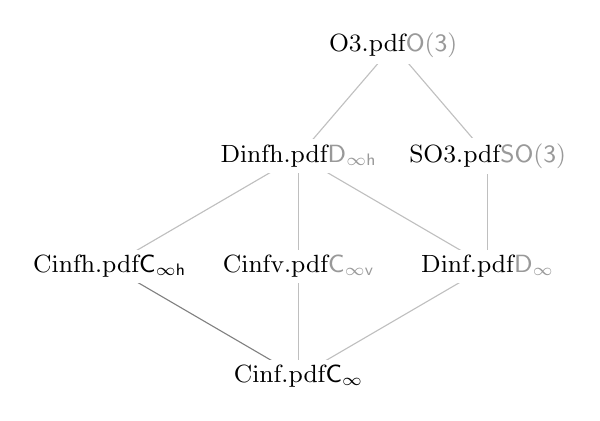
\begin{tikzpicture}[x=1cm, y=1cm, every node/.style={fill=white, font=\small, inner sep=2pt}]
\draw[black!50, line width=0.4pt] (0,0) -- (-2.4,1.4);
\draw[black!25, line width=0.4pt] (0,0) -- (0,1.4);
\draw[black!25, line width=0.4pt] (0,0) -- (2.4,1.4);
\draw[black!25, line width=0.4pt] (-2.4,1.4) -- (0,2.8);
\draw[black!25, line width=0.4pt] (0,1.4) -- (0,2.8);
\draw[black!25, line width=0.4pt] (2.4,1.4) -- (0,2.8);
\draw[black!25, line width=0.4pt] (2.4,1.4) -- (2.4,2.8);
\draw[black!25, line width=0.4pt] (0,2.8) -- (1.2,4.2);
\draw[black!25, line width=0.4pt] (2.4,2.8) -- (1.2,4.2);
\node at (0,0) {\href{Cinf.pdf}{\textcolor{black}{$\grp{C_{\infty}}$}}};
\node at (-2.4,1.4) {\href{Cinfh.pdf}{\textcolor{black}{$\grp{C_{\infty h}}$}}};
\node at (0,1.4) {\href{Cinfv.pdf}{\textcolor{black!40}{$\grp{C_{\infty v}}$}}};
\node at (2.4,1.4) {\href{Dinf.pdf}{\textcolor{black!40}{$\grp{D_{\infty}}$}}};
\node at (0,2.8) {\href{Dinfh.pdf}{\textcolor{black!40}{$\grp{D_{\infty h}}$}}};
\node at (2.4,2.8) {\href{SO3.pdf}{\textcolor{black!40}{$\grp{SO(3)}$}}};
\node at (1.2,4.2) {\href{O3.pdf}{\textcolor{black!40}{$\grp{O(3)}$}}};
\end{tikzpicture}\end{center}
\leavevmode\label{n:group.H}The table lists the closed subgroups $\grp{H}$ other than $\grp{C_{\infty h}}$ up to conjugacy in $\grp{C_{\infty h}}$, one in each row: the continuous subgroups, then the members of each family. Members of different families are not conjugate in $\grp{C_{\infty h}}$. A row with $N$ in its symbol stands for every $N$ of its range, and its entries are functions of $N$. \label{n:head.subgroup}\label{n:head.order}\label{n:head.conjugates}\label{n:head.normal}A row gives the representative $\grp{H}$ of a class of subgroups (subgrp), its order, the number of subgroups in the class (conjugates) and whether $\grp{H}$ is normal. \label{n:group.normalizer}\label{n:group.centralizer}It also gives the normalizer $\grp{N}_{\hairsp \grp{C_{\infty h}}}(\grp{H})$ and the centralizer $\grp{C}_{\hairsp \grp{C_{\infty h}}}(\grp{H})$ in $\grp{C_{\infty h}}$ (\texttt{normalizer}, \texttt{centralizer}). \label{n:head.components}The column components gives the components of the class space (section~\ref{s:class_space}) met by the subgroup. A subgroup's other names in its \href{O3.pdf}{$\grp{O(3)}$}-conjugacy class follow $\samecls$ (\href{../../CONVENTIONS.pdf}{CONVENTIONS.pdf}, section \href{../../CONVENTIONS.pdf\#conv.2.1}{2.1}).
{\small\setlength{\fillwidth}{\textwidth}\addtolength{\fillwidth}{-12\tabcolsep}\setlength{\colwidth}{0pt}\cellmax{$\grp{C_{1h}}$ $\samecls$ $\grp{C_{s}}$ $\samecls$ $\grp{C_{1v}}$}\cellmax{$\grp{C_{2h}}$ $\samecls$ $\grp{D_{1d}}$}\cellmax{$\grp{C_{\mathnormal{N}h}}$, $N \ge 3$}\cellmax{$\grp{S_{2\mathnormal{N}}}$, $N \ge 2$}\cellmax{$\grp{C_{2}}$ $\samecls$ $\grp{D_{1}}$}\cellmax{$\grp{C_{\mathnormal{N}}}$, $N \ge 3$}\cellmax{$\grp{S_{2}}$ $\samecls$ $\grp{C_{i}}$}\cellmax{subgrp}\cellmax{$\grp{C_{1}}$}\cellmax{$\grp{C_{\infty}}$}\addtolength{\fillwidth}{-\colwidth}\setlength{\colwidth}{0pt}\cellmax{order}\cellmax{$2N$}\cellmax{$N$}\cellmax{$\infty$}\cellmax{1}\cellmax{2}\cellmax{4}\addtolength{\fillwidth}{-\colwidth}\setlength{\colwidth}{0pt}\cellmax{conjugates}\cellmax{1}\addtolength{\fillwidth}{-\colwidth}\setlength{\colwidth}{0pt}\cellmax{normal}\cellmax{yes}\addtolength{\fillwidth}{-\colwidth}\setlength{\colwidth}{0pt}\cellmax{$\grp{N}_{\hairsp \grp{C_{\infty h}}}(\grp{H})$}\cellmax{$\grp{C_{\infty h}}$}\addtolength{\fillwidth}{-\colwidth}\setlength{\colwidth}{0pt}\cellmax{$\grp{C}_{\hairsp \grp{C_{\infty h}}}(\grp{H})$}\cellmax{$\grp{C_{\infty h}}$}\addtolength{\fillwidth}{-\colwidth}\setlength{\colwidth}{0pt}\cellmax{$\comp{C_{\infty}(\phi)}$, $\comp{i\,C_{\infty}(\phi)}$}\cellmax{components}\cellmax{$\comp{C_{\infty}(\phi)}$}\fillcap\begin{longtable}{@{}lrrlll>{\RaggedRight\arraybackslash}p{\fillwidth}@{}}\toprule
subgrp & order & conjugates & normal & $\grp{N}_{\hairsp \grp{C_{\infty h}}}(\grp{H})$ & $\grp{C}_{\hairsp \grp{C_{\infty h}}}(\grp{H})$ & components\\\midrule\endhead
\bottomrule\endfoot\endlastfoot
\href{Cinf.pdf}{$\grp{C_{\infty}}$} & $\infty$ & 1 & yes & \href{Cinfh.pdf}{$\grp{C_{\infty h}}$} & \href{Cinfh.pdf}{$\grp{C_{\infty h}}$} & $\comp{C_{\infty}(\phi)}$\\*
\grouprule{0pt}{\lightrulewidth}
\href{C1.pdf}{$\grp{C_{1}}$} & 1 & 1 & yes & \href{Cinfh.pdf}{$\grp{C_{\infty h}}$} & \href{Cinfh.pdf}{$\grp{C_{\infty h}}$} & $\comp{C_{\infty}(\phi)}$\\
\href{C2.pdf}{$\grp{C_{2}}$} $\samecls$ \href{D1.pdf}{$\grp{D_{1}}$} & 2 & 1 & yes & \href{Cinfh.pdf}{$\grp{C_{\infty h}}$} & \href{Cinfh.pdf}{$\grp{C_{\infty h}}$} & $\comp{C_{\infty}(\phi)}$\\
$\grp{C_{\mathnormal{N}}}$, $N \ge 3$ & $N$ & 1 & yes & \href{Cinfh.pdf}{$\grp{C_{\infty h}}$} & \href{Cinfh.pdf}{$\grp{C_{\infty h}}$} & $\comp{C_{\infty}(\phi)}$\\
\grouprule{0pt}{\lightrulewidth}
\href{S2.pdf}{$\grp{S_{2}}$} $\samecls$ \href{S2.pdf}{$\grp{C_{i}}$} & 2 & 1 & yes & \href{Cinfh.pdf}{$\grp{C_{\infty h}}$} & \href{Cinfh.pdf}{$\grp{C_{\infty h}}$} & $\comp{C_{\infty}(\phi)}$, $\comp{i\,C_{\infty}(\phi)}$\\
$\grp{S_{2\mathnormal{N}}}$, $N \ge 2$ & $2N$ & 1 & yes & \href{Cinfh.pdf}{$\grp{C_{\infty h}}$} & \href{Cinfh.pdf}{$\grp{C_{\infty h}}$} & $\comp{C_{\infty}(\phi)}$, $\comp{i\,C_{\infty}(\phi)}$\\
\grouprule{0pt}{\lightrulewidth}
\href{C1h.pdf}{$\grp{C_{1h}}$} $\samecls$ \href{C1v.pdf}{$\grp{C_{s}}$} $\samecls$ \href{C1v.pdf}{$\grp{C_{1v}}$} & 2 & 1 & yes & \href{Cinfh.pdf}{$\grp{C_{\infty h}}$} & \href{Cinfh.pdf}{$\grp{C_{\infty h}}$} & $\comp{C_{\infty}(\phi)}$, $\comp{i\,C_{\infty}(\phi)}$\\
\href{C2h.pdf}{$\grp{C_{2h}}$} $\samecls$ \href{D1d.pdf}{$\grp{D_{1d}}$} & 4 & 1 & yes & \href{Cinfh.pdf}{$\grp{C_{\infty h}}$} & \href{Cinfh.pdf}{$\grp{C_{\infty h}}$} & $\comp{C_{\infty}(\phi)}$, $\comp{i\,C_{\infty}(\phi)}$\\*
$\grp{C_{\mathnormal{N}h}}$, $N \ge 3$ & $2N$ & 1 & yes & \href{Cinfh.pdf}{$\grp{C_{\infty h}}$} & \href{Cinfh.pdf}{$\grp{C_{\infty h}}$} & $\comp{C_{\infty}(\phi)}$, $\comp{i\,C_{\infty}(\phi)}$\\
\bottomrule\end{longtable}}
\needspace{103pt}
\section{Descent of symmetry}\label{s:subduction}
Conventions: \href{../../CONVENTIONS.pdf}{CONVENTIONS.pdf}, section \href{../../CONVENTIONS.pdf\#conv.16.1}{16.1}.
The closed subgroups of $\grp{C_{\infty h}}$ other than $\grp{C_{\infty h}}$, up to conjugacy in $\grp{C_{\infty h}}$, are its continuous subgroups and, for every $N \ge 1$, one subgroup for each member of each family of section~\ref{s:subgroups}. The subgroup for a member is the group of that member's document, in its own frame. Members of different families are not conjugate in $\grp{C_{\infty h}}$. The entry of row $\Gamma$ is $\restr{\Gamma}{\grp{H}}$ as a sum of the irreps of $\grp{H}$.
\needspace{149pt}
\paragraph{Continuous subgroups.} \label{n:head.index.subgroup}The row subgrp gives each continuous subgroup $\grp{H}$, and the row index gives its index $\grpindex{\grp{C_{\infty h}}}{\grp{H}}$. The intertwiners (\texttt{subduction\symbol{95}subgroups.continuous[]}) are the identity.
{\small\begin{longtable}{@{}lc@{}}\toprule
subgrp & \href{Cinf.pdf}{$\grp{C_{\infty}}$}\\
index & 2\\\midrule\endhead
\bottomrule\endfoot\endlastfoot
$\irr{a}_{\ptag{g}}$ & $\irr{a}$\\*
$\conjpair{1}\irr{e}_{n,\ptag{g}}$ & $\conjpair{1}\irr{e}_{n}$\\*
$\conjpair{2}\irr{e}_{n,\ptag{g}}$ & $\conjpair{2}\irr{e}_{n}$\\*
$\irr{a}_{\ptag{u}}$ & $\irr{a}$\\*
$\conjpair{1}\irr{e}_{n,\ptag{u}}$ & $\conjpair{1}\irr{e}_{n}$\\*
$\conjpair{2}\irr{e}_{n,\ptag{u}}$ & $\conjpair{2}\irr{e}_{n}$\\
\bottomrule\end{longtable}}
\needspace{116pt}
\paragraph{Finite subgroups.} \label{n:function.character.plain}\label{n:element.principal}\label{n:constant.root}\label{n:index.residue}\label{n:index.order.principal}For each family, the rule gives the restriction for every $N$ as the irrep with $\chi(g_p) = \rootunity{N_p}^{q}$ (the pair $\rootunity{N_p}^{\pm q}$ for an $\irr{e}_n$), labeled as in \href{../../CONVENTIONS.pdf}{CONVENTIONS.pdf}, section \href{../../CONVENTIONS.pdf\#conv.6.1}{6.1}. Here $\rootunity{N_p} = \expe^{2\pi\iunit/N_p}$, where $g_p = \elt{C_\infty}(2\pi/N)$ and $N_p = N$, or $g_p = \elt{\sigma_h C_\infty}(\pi/N)$ and $N_p = 2N$ in $\grp{S_{2\mathnormal{N}}}$ with $N$ even. For $N = 1$ and $2$ the irreps are named as in \href{../../CONVENTIONS.pdf}{CONVENTIONS.pdf}, section \href{../../CONVENTIONS.pdf\#conv.6.3}{6.3}. \label{n:index.period}The restriction of the instance $n$ depends on $n$ only modulo the period $\period$ of the member. The tables list $N \le 12$ and $n \le 6$, and the record holds $n = 1, 2, \dots, \period$ with the intertwiners (\texttt{subduction\symbol{95}subgroups.finite[]}). \label{n:group.normalizer.o3}\label{n:group.centralizer.o3}\label{n:element.h}The record of $\grp{H}$ maps onto the subgroup in $\grpindex{\grp{N}}{\grp{C}}$ ways, $h \mapsto g h g^{-1}$ ($h \in \grp{H}$) for the $g \in \grp{O(3)}$ that carry $\grp{H}$ to it. Here $\grp{N}$ and $\grp{C}$ are the normalizer and centralizer of $\grp{H}$ in \href{O3.pdf}{$\grp{O(3)}$}. In the section Names and structure of the document of $\grp{H}$, the row centralizer gives $\grp{C}$ and the index $\grpindex{\grp{N}}{\grp{C}}$ (the index in the row normalizer is $\grpindex{\grp{N}}{\grp{H}}$). Two maps related by a conjugation in $\grp{C_{\infty h}}$ give the same restriction. Thus the maps fall into $\grpindex{\grp{N}}{\grp{C}}/\grpindex{\grp{N}_{\hairsp \grp{C_{\infty h}}}}{\grp{C}_{\hairsp \grp{C_{\infty h}}}}$ classes, where $\grp{N}_{\hairsp \grp{C_{\infty h}}}$ and $\grp{C}_{\hairsp \grp{C_{\infty h}}}$ are the normalizer and centralizer of the subgroup in $\grp{C_{\infty h}}$ (the table of section~\ref{s:subgroups}). \label{n:head.setting}A subgroup whose classes of maps give different tables has one column for each table: setting 1 for the stored monomorphism (\texttt{monomorphism}) and settings 2, 3, \dots{} for the \texttt{alternative\symbol{95}settings}. Each setting has the images of the generators of $\grp{H}$ (\texttt{setting}). \label{n:head.images}The row images gives, under each setting, each generator whose image differs between the settings, in their order, mapped to its image. Each image is the element of its component of the class space at its angle. Each generator is written by the symbol of its class (\href{../../CONVENTIONS.pdf}{CONVENTIONS.pdf}, section \href{../../CONVENTIONS.pdf\#conv.5.1}{5.1}), and where two share a symbol, a superscript number in brackets gives the generator's index in the document of $\grp{H}$. \label{n:irrep.Delta}Each other setting is setting 1 with each irrep $\Lambda$ of $\grp{H}$ replaced by $\Lambda$ composed with one automorphism of $\grp{H}$ induced by a conjugation in \href{O3.pdf}{$\grp{O(3)}$} and by none in $\grp{C_{\infty h}}$ (\href{../../CONVENTIONS.pdf}{CONVENTIONS.pdf}, section \href{../../CONVENTIONS.pdf\#conv.12.1}{12.1}).

\needspace{95pt}
\paragraph{Subduction to the $\grp{C_{\mathnormal{N}}}$ family.}
{\small\setlength{\fillwidth}{\textwidth}\addtolength{\fillwidth}{-2\tabcolsep}\setlength{\colwidth}{0pt}\cellmax{$\conjpair{1}\irr{e}_{n,\ptag{g}}$}\cellmax{$\conjpair{1}\irr{e}_{n,\ptag{u}}$}\cellmax{$\conjpair{2}\irr{e}_{n,\ptag{g}}$}\cellmax{$\conjpair{2}\irr{e}_{n,\ptag{u}}$}\cellmax{$\irr{a}_{\ptag{g}}$}\cellmax{$\irr{a}_{\ptag{u}}$}\addtolength{\fillwidth}{-\colwidth}\setlength{\colwidth}{0pt}\cellmax{$\irr{a}$ if $q = 0$, $\irr{b}$ if $q = N/2$, $\conjpair{1}\irr{e}_{q}$ if $0 < q < N/2$, $\conjpair{2}\irr{e}_{N-q}$ if $N/2 < q < N$; $q = -n \bmod N$}\cellmax{$\irr{a}$ if $q = 0$, $\irr{b}$ if $q = N/2$, $\conjpair{1}\irr{e}_{q}$ if $0 < q < N/2$, $\conjpair{2}\irr{e}_{N-q}$ if $N/2 < q < N$; $q = n \bmod N$}\cellmax{$\irr{a}$}\fillcap\begin{longtable}{@{}l>{\raggedright\arraybackslash}p{\fillwidth}@{}}\toprule
\multicolumn{2}{@{}c@{}}{every $N$}\\*
$\irr{a}_{\ptag{g}}$ & $\irr{a}$\\*
$\conjpair{1}\irr{e}_{n,\ptag{g}}$ & $\irr{a}$ if $q = 0$, $\irr{b}$ if $q = N/2$, $\conjpair{1}\irr{e}_{q}$ if $0 < q < N/2$, $\conjpair{2}\irr{e}_{N-q}$ if $N/2 < q < N$; $q = n \bmod N$\\*
$\conjpair{2}\irr{e}_{n,\ptag{g}}$ & $\irr{a}$ if $q = 0$, $\irr{b}$ if $q = N/2$, $\conjpair{1}\irr{e}_{q}$ if $0 < q < N/2$, $\conjpair{2}\irr{e}_{N-q}$ if $N/2 < q < N$; $q = -n \bmod N$\\*
$\irr{a}_{\ptag{u}}$ & $\irr{a}$\\*
$\conjpair{1}\irr{e}_{n,\ptag{u}}$ & $\irr{a}$ if $q = 0$, $\irr{b}$ if $q = N/2$, $\conjpair{1}\irr{e}_{q}$ if $0 < q < N/2$, $\conjpair{2}\irr{e}_{N-q}$ if $N/2 < q < N$; $q = n \bmod N$\\*
$\conjpair{2}\irr{e}_{n,\ptag{u}}$ & $\irr{a}$ if $q = 0$, $\irr{b}$ if $q = N/2$, $\conjpair{1}\irr{e}_{q}$ if $0 < q < N/2$, $\conjpair{2}\irr{e}_{N-q}$ if $N/2 < q < N$; $q = -n \bmod N$\\
\bottomrule\end{longtable}}
{\small\begin{longtable}{@{}lccccccc@{}}\toprule
subgrp & \href{C2.pdf}{$\grp{C_{2}}$} & \multicolumn{2}{c}{\href{C3.pdf}{$\grp{C_{3}}$}} & \multicolumn{2}{c}{\href{C4.pdf}{$\grp{C_{4}}$}} & \multicolumn{2}{c}{\href{C5.pdf}{$\grp{C_{5}}$}}\\\cmidrule(lr){3-4}\cmidrule(lr){5-6}\cmidrule(lr){7-8}
setting &  & 1 & 2 & 1 & 2 & 1 & 2\\
images &  & {\scriptsize $\cls{C_{3}} \mapsto \elt{C_{\infty}}(2\pi/3)$} & {\scriptsize $\cls{C_{3}} \mapsto \elt{C_{\infty}}(4\pi/3)$} & {\scriptsize $\cls{C_{4}} \mapsto \elt{C_{\infty}}(\pi/2)$} & {\scriptsize $\cls{C_{4}} \mapsto \elt{C_{\infty}}(3\pi/2)$} & {\scriptsize $\cls{C_{5}} \mapsto \elt{C_{\infty}}(2\pi/5)$} & {\scriptsize $\cls{C_{5}} \mapsto \elt{C_{\infty}}(8\pi/5)$}\\\midrule\endhead
\bottomrule\endfoot\endlastfoot
$\irr{a}_{\ptag{g}}$ & $\irr{a}$ & $\irr{a}$ & $\irr{a}$ & $\irr{a}$ & $\irr{a}$ & $\irr{a}$ & $\irr{a}$\\*
$\conjpair{1}\irr{e}_{1\ptag{g}}$ & $\irr{b}$ & $\conjpair{1}\irr{e}$ & $\conjpair{2}\irr{e}$ & $\conjpair{1}\irr{e}$ & $\conjpair{2}\irr{e}$ & $\conjpair{1}\irr{e}_{1}$ & $\conjpair{2}\irr{e}_{1}$\\
$\conjpair{1}\irr{e}_{2\ptag{g}}$ & $\irr{a}$ & $\conjpair{2}\irr{e}$ & $\conjpair{1}\irr{e}$ & $\irr{b}$ & $\irr{b}$ & $\conjpair{1}\irr{e}_{2}$ & $\conjpair{2}\irr{e}_{2}$\\
$\conjpair{1}\irr{e}_{3\ptag{g}}$ & $\irr{b}$ & $\irr{a}$ & $\irr{a}$ & $\conjpair{2}\irr{e}$ & $\conjpair{1}\irr{e}$ & $\conjpair{2}\irr{e}_{2}$ & $\conjpair{1}\irr{e}_{2}$\\
$\conjpair{1}\irr{e}_{4\ptag{g}}$ & $\irr{a}$ & $\conjpair{1}\irr{e}$ & $\conjpair{2}\irr{e}$ & $\irr{a}$ & $\irr{a}$ & $\conjpair{2}\irr{e}_{1}$ & $\conjpair{1}\irr{e}_{1}$\\
$\conjpair{1}\irr{e}_{5\ptag{g}}$ & $\irr{b}$ & $\conjpair{2}\irr{e}$ & $\conjpair{1}\irr{e}$ & $\conjpair{1}\irr{e}$ & $\conjpair{2}\irr{e}$ & $\irr{a}$ & $\irr{a}$\\
$\conjpair{1}\irr{e}_{6\ptag{g}}$ & $\irr{a}$ & $\irr{a}$ & $\irr{a}$ & $\irr{b}$ & $\irr{b}$ & $\conjpair{1}\irr{e}_{1}$ & $\conjpair{2}\irr{e}_{1}$\\
$\conjpair{2}\irr{e}_{1\ptag{g}}$ & $\irr{b}$ & $\conjpair{2}\irr{e}$ & $\conjpair{1}\irr{e}$ & $\conjpair{2}\irr{e}$ & $\conjpair{1}\irr{e}$ & $\conjpair{2}\irr{e}_{1}$ & $\conjpair{1}\irr{e}_{1}$\\
$\conjpair{2}\irr{e}_{2\ptag{g}}$ & $\irr{a}$ & $\conjpair{1}\irr{e}$ & $\conjpair{2}\irr{e}$ & $\irr{b}$ & $\irr{b}$ & $\conjpair{2}\irr{e}_{2}$ & $\conjpair{1}\irr{e}_{2}$\\
$\conjpair{2}\irr{e}_{3\ptag{g}}$ & $\irr{b}$ & $\irr{a}$ & $\irr{a}$ & $\conjpair{1}\irr{e}$ & $\conjpair{2}\irr{e}$ & $\conjpair{1}\irr{e}_{2}$ & $\conjpair{2}\irr{e}_{2}$\\
$\conjpair{2}\irr{e}_{4\ptag{g}}$ & $\irr{a}$ & $\conjpair{2}\irr{e}$ & $\conjpair{1}\irr{e}$ & $\irr{a}$ & $\irr{a}$ & $\conjpair{1}\irr{e}_{1}$ & $\conjpair{2}\irr{e}_{1}$\\
$\conjpair{2}\irr{e}_{5\ptag{g}}$ & $\irr{b}$ & $\conjpair{1}\irr{e}$ & $\conjpair{2}\irr{e}$ & $\conjpair{2}\irr{e}$ & $\conjpair{1}\irr{e}$ & $\irr{a}$ & $\irr{a}$\\
$\conjpair{2}\irr{e}_{6\ptag{g}}$ & $\irr{a}$ & $\irr{a}$ & $\irr{a}$ & $\irr{b}$ & $\irr{b}$ & $\conjpair{2}\irr{e}_{1}$ & $\conjpair{1}\irr{e}_{1}$\\
$\irr{a}_{\ptag{u}}$ & $\irr{a}$ & $\irr{a}$ & $\irr{a}$ & $\irr{a}$ & $\irr{a}$ & $\irr{a}$ & $\irr{a}$\\
$\conjpair{1}\irr{e}_{1\ptag{u}}$ & $\irr{b}$ & $\conjpair{1}\irr{e}$ & $\conjpair{2}\irr{e}$ & $\conjpair{1}\irr{e}$ & $\conjpair{2}\irr{e}$ & $\conjpair{1}\irr{e}_{1}$ & $\conjpair{2}\irr{e}_{1}$\\
$\conjpair{1}\irr{e}_{2\ptag{u}}$ & $\irr{a}$ & $\conjpair{2}\irr{e}$ & $\conjpair{1}\irr{e}$ & $\irr{b}$ & $\irr{b}$ & $\conjpair{1}\irr{e}_{2}$ & $\conjpair{2}\irr{e}_{2}$\\
$\conjpair{1}\irr{e}_{3\ptag{u}}$ & $\irr{b}$ & $\irr{a}$ & $\irr{a}$ & $\conjpair{2}\irr{e}$ & $\conjpair{1}\irr{e}$ & $\conjpair{2}\irr{e}_{2}$ & $\conjpair{1}\irr{e}_{2}$\\
$\conjpair{1}\irr{e}_{4\ptag{u}}$ & $\irr{a}$ & $\conjpair{1}\irr{e}$ & $\conjpair{2}\irr{e}$ & $\irr{a}$ & $\irr{a}$ & $\conjpair{2}\irr{e}_{1}$ & $\conjpair{1}\irr{e}_{1}$\\
$\conjpair{1}\irr{e}_{5\ptag{u}}$ & $\irr{b}$ & $\conjpair{2}\irr{e}$ & $\conjpair{1}\irr{e}$ & $\conjpair{1}\irr{e}$ & $\conjpair{2}\irr{e}$ & $\irr{a}$ & $\irr{a}$\\
$\conjpair{1}\irr{e}_{6\ptag{u}}$ & $\irr{a}$ & $\irr{a}$ & $\irr{a}$ & $\irr{b}$ & $\irr{b}$ & $\conjpair{1}\irr{e}_{1}$ & $\conjpair{2}\irr{e}_{1}$\\
$\conjpair{2}\irr{e}_{1\ptag{u}}$ & $\irr{b}$ & $\conjpair{2}\irr{e}$ & $\conjpair{1}\irr{e}$ & $\conjpair{2}\irr{e}$ & $\conjpair{1}\irr{e}$ & $\conjpair{2}\irr{e}_{1}$ & $\conjpair{1}\irr{e}_{1}$\\
$\conjpair{2}\irr{e}_{2\ptag{u}}$ & $\irr{a}$ & $\conjpair{1}\irr{e}$ & $\conjpair{2}\irr{e}$ & $\irr{b}$ & $\irr{b}$ & $\conjpair{2}\irr{e}_{2}$ & $\conjpair{1}\irr{e}_{2}$\\
$\conjpair{2}\irr{e}_{3\ptag{u}}$ & $\irr{b}$ & $\irr{a}$ & $\irr{a}$ & $\conjpair{1}\irr{e}$ & $\conjpair{2}\irr{e}$ & $\conjpair{1}\irr{e}_{2}$ & $\conjpair{2}\irr{e}_{2}$\\
$\conjpair{2}\irr{e}_{4\ptag{u}}$ & $\irr{a}$ & $\conjpair{2}\irr{e}$ & $\conjpair{1}\irr{e}$ & $\irr{a}$ & $\irr{a}$ & $\conjpair{1}\irr{e}_{1}$ & $\conjpair{2}\irr{e}_{1}$\\
$\conjpair{2}\irr{e}_{5\ptag{u}}$ & $\irr{b}$ & $\conjpair{1}\irr{e}$ & $\conjpair{2}\irr{e}$ & $\conjpair{2}\irr{e}$ & $\conjpair{1}\irr{e}$ & $\irr{a}$ & $\irr{a}$\\*
$\conjpair{2}\irr{e}_{6\ptag{u}}$ & $\irr{a}$ & $\irr{a}$ & $\irr{a}$ & $\irr{b}$ & $\irr{b}$ & $\conjpair{2}\irr{e}_{1}$ & $\conjpair{1}\irr{e}_{1}$\\
\bottomrule\end{longtable}}
{\small\begin{longtable}{@{}lcccccc@{}}\toprule
subgrp & \multicolumn{2}{c}{\href{C6.pdf}{$\grp{C_{6}}$}} & \multicolumn{2}{c}{\href{C7.pdf}{$\grp{C_{7}}$}} & \multicolumn{2}{c}{\href{C8.pdf}{$\grp{C_{8}}$}}\\\cmidrule(lr){2-3}\cmidrule(lr){4-5}\cmidrule(lr){6-7}
setting & 1 & 2 & 1 & 2 & 1 & 2\\
images & {\scriptsize $\cls{C_{6}} \mapsto \elt{C_{\infty}}(\pi/3)$} & {\scriptsize $\cls{C_{6}} \mapsto \elt{C_{\infty}}(5\pi/3)$} & {\scriptsize $\cls{C_{7}} \mapsto \elt{C_{\infty}}(2\pi/7)$} & {\scriptsize $\cls{C_{7}} \mapsto \elt{C_{\infty}}(12\pi/7)$} & {\scriptsize $\cls{C_{8}} \mapsto \elt{C_{\infty}}(\pi/4)$} & {\scriptsize $\cls{C_{8}} \mapsto \elt{C_{\infty}}(7\pi/4)$}\\\midrule\endhead
\bottomrule\endfoot\endlastfoot
$\irr{a}_{\ptag{g}}$ & $\irr{a}$ & $\irr{a}$ & $\irr{a}$ & $\irr{a}$ & $\irr{a}$ & $\irr{a}$\\*
$\conjpair{1}\irr{e}_{1\ptag{g}}$ & $\conjpair{1}\irr{e}_{1}$ & $\conjpair{2}\irr{e}_{1}$ & $\conjpair{1}\irr{e}_{1}$ & $\conjpair{2}\irr{e}_{1}$ & $\conjpair{1}\irr{e}_{1}$ & $\conjpair{2}\irr{e}_{1}$\\
$\conjpair{1}\irr{e}_{2\ptag{g}}$ & $\conjpair{1}\irr{e}_{2}$ & $\conjpair{2}\irr{e}_{2}$ & $\conjpair{1}\irr{e}_{2}$ & $\conjpair{2}\irr{e}_{2}$ & $\conjpair{1}\irr{e}_{2}$ & $\conjpair{2}\irr{e}_{2}$\\
$\conjpair{1}\irr{e}_{3\ptag{g}}$ & $\irr{b}$ & $\irr{b}$ & $\conjpair{1}\irr{e}_{3}$ & $\conjpair{2}\irr{e}_{3}$ & $\conjpair{1}\irr{e}_{3}$ & $\conjpair{2}\irr{e}_{3}$\\
$\conjpair{1}\irr{e}_{4\ptag{g}}$ & $\conjpair{2}\irr{e}_{2}$ & $\conjpair{1}\irr{e}_{2}$ & $\conjpair{2}\irr{e}_{3}$ & $\conjpair{1}\irr{e}_{3}$ & $\irr{b}$ & $\irr{b}$\\
$\conjpair{1}\irr{e}_{5\ptag{g}}$ & $\conjpair{2}\irr{e}_{1}$ & $\conjpair{1}\irr{e}_{1}$ & $\conjpair{2}\irr{e}_{2}$ & $\conjpair{1}\irr{e}_{2}$ & $\conjpair{2}\irr{e}_{3}$ & $\conjpair{1}\irr{e}_{3}$\\
$\conjpair{1}\irr{e}_{6\ptag{g}}$ & $\irr{a}$ & $\irr{a}$ & $\conjpair{2}\irr{e}_{1}$ & $\conjpair{1}\irr{e}_{1}$ & $\conjpair{2}\irr{e}_{2}$ & $\conjpair{1}\irr{e}_{2}$\\
$\conjpair{2}\irr{e}_{1\ptag{g}}$ & $\conjpair{2}\irr{e}_{1}$ & $\conjpair{1}\irr{e}_{1}$ & $\conjpair{2}\irr{e}_{1}$ & $\conjpair{1}\irr{e}_{1}$ & $\conjpair{2}\irr{e}_{1}$ & $\conjpair{1}\irr{e}_{1}$\\
$\conjpair{2}\irr{e}_{2\ptag{g}}$ & $\conjpair{2}\irr{e}_{2}$ & $\conjpair{1}\irr{e}_{2}$ & $\conjpair{2}\irr{e}_{2}$ & $\conjpair{1}\irr{e}_{2}$ & $\conjpair{2}\irr{e}_{2}$ & $\conjpair{1}\irr{e}_{2}$\\
$\conjpair{2}\irr{e}_{3\ptag{g}}$ & $\irr{b}$ & $\irr{b}$ & $\conjpair{2}\irr{e}_{3}$ & $\conjpair{1}\irr{e}_{3}$ & $\conjpair{2}\irr{e}_{3}$ & $\conjpair{1}\irr{e}_{3}$\\
$\conjpair{2}\irr{e}_{4\ptag{g}}$ & $\conjpair{1}\irr{e}_{2}$ & $\conjpair{2}\irr{e}_{2}$ & $\conjpair{1}\irr{e}_{3}$ & $\conjpair{2}\irr{e}_{3}$ & $\irr{b}$ & $\irr{b}$\\
$\conjpair{2}\irr{e}_{5\ptag{g}}$ & $\conjpair{1}\irr{e}_{1}$ & $\conjpair{2}\irr{e}_{1}$ & $\conjpair{1}\irr{e}_{2}$ & $\conjpair{2}\irr{e}_{2}$ & $\conjpair{1}\irr{e}_{3}$ & $\conjpair{2}\irr{e}_{3}$\\
$\conjpair{2}\irr{e}_{6\ptag{g}}$ & $\irr{a}$ & $\irr{a}$ & $\conjpair{1}\irr{e}_{1}$ & $\conjpair{2}\irr{e}_{1}$ & $\conjpair{1}\irr{e}_{2}$ & $\conjpair{2}\irr{e}_{2}$\\
$\irr{a}_{\ptag{u}}$ & $\irr{a}$ & $\irr{a}$ & $\irr{a}$ & $\irr{a}$ & $\irr{a}$ & $\irr{a}$\\
$\conjpair{1}\irr{e}_{1\ptag{u}}$ & $\conjpair{1}\irr{e}_{1}$ & $\conjpair{2}\irr{e}_{1}$ & $\conjpair{1}\irr{e}_{1}$ & $\conjpair{2}\irr{e}_{1}$ & $\conjpair{1}\irr{e}_{1}$ & $\conjpair{2}\irr{e}_{1}$\\
$\conjpair{1}\irr{e}_{2\ptag{u}}$ & $\conjpair{1}\irr{e}_{2}$ & $\conjpair{2}\irr{e}_{2}$ & $\conjpair{1}\irr{e}_{2}$ & $\conjpair{2}\irr{e}_{2}$ & $\conjpair{1}\irr{e}_{2}$ & $\conjpair{2}\irr{e}_{2}$\\
$\conjpair{1}\irr{e}_{3\ptag{u}}$ & $\irr{b}$ & $\irr{b}$ & $\conjpair{1}\irr{e}_{3}$ & $\conjpair{2}\irr{e}_{3}$ & $\conjpair{1}\irr{e}_{3}$ & $\conjpair{2}\irr{e}_{3}$\\
$\conjpair{1}\irr{e}_{4\ptag{u}}$ & $\conjpair{2}\irr{e}_{2}$ & $\conjpair{1}\irr{e}_{2}$ & $\conjpair{2}\irr{e}_{3}$ & $\conjpair{1}\irr{e}_{3}$ & $\irr{b}$ & $\irr{b}$\\
$\conjpair{1}\irr{e}_{5\ptag{u}}$ & $\conjpair{2}\irr{e}_{1}$ & $\conjpair{1}\irr{e}_{1}$ & $\conjpair{2}\irr{e}_{2}$ & $\conjpair{1}\irr{e}_{2}$ & $\conjpair{2}\irr{e}_{3}$ & $\conjpair{1}\irr{e}_{3}$\\
$\conjpair{1}\irr{e}_{6\ptag{u}}$ & $\irr{a}$ & $\irr{a}$ & $\conjpair{2}\irr{e}_{1}$ & $\conjpair{1}\irr{e}_{1}$ & $\conjpair{2}\irr{e}_{2}$ & $\conjpair{1}\irr{e}_{2}$\\
$\conjpair{2}\irr{e}_{1\ptag{u}}$ & $\conjpair{2}\irr{e}_{1}$ & $\conjpair{1}\irr{e}_{1}$ & $\conjpair{2}\irr{e}_{1}$ & $\conjpair{1}\irr{e}_{1}$ & $\conjpair{2}\irr{e}_{1}$ & $\conjpair{1}\irr{e}_{1}$\\
$\conjpair{2}\irr{e}_{2\ptag{u}}$ & $\conjpair{2}\irr{e}_{2}$ & $\conjpair{1}\irr{e}_{2}$ & $\conjpair{2}\irr{e}_{2}$ & $\conjpair{1}\irr{e}_{2}$ & $\conjpair{2}\irr{e}_{2}$ & $\conjpair{1}\irr{e}_{2}$\\
$\conjpair{2}\irr{e}_{3\ptag{u}}$ & $\irr{b}$ & $\irr{b}$ & $\conjpair{2}\irr{e}_{3}$ & $\conjpair{1}\irr{e}_{3}$ & $\conjpair{2}\irr{e}_{3}$ & $\conjpair{1}\irr{e}_{3}$\\
$\conjpair{2}\irr{e}_{4\ptag{u}}$ & $\conjpair{1}\irr{e}_{2}$ & $\conjpair{2}\irr{e}_{2}$ & $\conjpair{1}\irr{e}_{3}$ & $\conjpair{2}\irr{e}_{3}$ & $\irr{b}$ & $\irr{b}$\\
$\conjpair{2}\irr{e}_{5\ptag{u}}$ & $\conjpair{1}\irr{e}_{1}$ & $\conjpair{2}\irr{e}_{1}$ & $\conjpair{1}\irr{e}_{2}$ & $\conjpair{2}\irr{e}_{2}$ & $\conjpair{1}\irr{e}_{3}$ & $\conjpair{2}\irr{e}_{3}$\\*
$\conjpair{2}\irr{e}_{6\ptag{u}}$ & $\irr{a}$ & $\irr{a}$ & $\conjpair{1}\irr{e}_{1}$ & $\conjpair{2}\irr{e}_{1}$ & $\conjpair{1}\irr{e}_{2}$ & $\conjpair{2}\irr{e}_{2}$\\
\bottomrule\end{longtable}}
{\small\begin{longtable}{@{}lcccc@{}}\toprule
subgrp & \multicolumn{2}{c}{\href{C9.pdf}{$\grp{C_{9}}$}} & \multicolumn{2}{c}{\href{C10.pdf}{$\grp{C_{10}}$}}\\\cmidrule(lr){2-3}\cmidrule(lr){4-5}
setting & 1 & 2 & 1 & 2\\
images & {\scriptsize $\cls{C_{9}} \mapsto \elt{C_{\infty}}(2\pi/9)$} & {\scriptsize $\cls{C_{9}} \mapsto \elt{C_{\infty}}(16\pi/9)$} & {\scriptsize $\cls{C_{10}} \mapsto \elt{C_{\infty}}(\pi/5)$} & {\scriptsize $\cls{C_{10}} \mapsto \elt{C_{\infty}}(9\pi/5)$}\\\midrule\endhead
\bottomrule\endfoot\endlastfoot
$\irr{a}_{\ptag{g}}$ & $\irr{a}$ & $\irr{a}$ & $\irr{a}$ & $\irr{a}$\\*
$\conjpair{1}\irr{e}_{1\ptag{g}}$ & $\conjpair{1}\irr{e}_{1}$ & $\conjpair{2}\irr{e}_{1}$ & $\conjpair{1}\irr{e}_{1}$ & $\conjpair{2}\irr{e}_{1}$\\
$\conjpair{1}\irr{e}_{2\ptag{g}}$ & $\conjpair{1}\irr{e}_{2}$ & $\conjpair{2}\irr{e}_{2}$ & $\conjpair{1}\irr{e}_{2}$ & $\conjpair{2}\irr{e}_{2}$\\
$\conjpair{1}\irr{e}_{3\ptag{g}}$ & $\conjpair{1}\irr{e}_{3}$ & $\conjpair{2}\irr{e}_{3}$ & $\conjpair{1}\irr{e}_{3}$ & $\conjpair{2}\irr{e}_{3}$\\
$\conjpair{1}\irr{e}_{4\ptag{g}}$ & $\conjpair{1}\irr{e}_{4}$ & $\conjpair{2}\irr{e}_{4}$ & $\conjpair{1}\irr{e}_{4}$ & $\conjpair{2}\irr{e}_{4}$\\
$\conjpair{1}\irr{e}_{5\ptag{g}}$ & $\conjpair{2}\irr{e}_{4}$ & $\conjpair{1}\irr{e}_{4}$ & $\irr{b}$ & $\irr{b}$\\
$\conjpair{1}\irr{e}_{6\ptag{g}}$ & $\conjpair{2}\irr{e}_{3}$ & $\conjpair{1}\irr{e}_{3}$ & $\conjpair{2}\irr{e}_{4}$ & $\conjpair{1}\irr{e}_{4}$\\
$\conjpair{2}\irr{e}_{1\ptag{g}}$ & $\conjpair{2}\irr{e}_{1}$ & $\conjpair{1}\irr{e}_{1}$ & $\conjpair{2}\irr{e}_{1}$ & $\conjpair{1}\irr{e}_{1}$\\
$\conjpair{2}\irr{e}_{2\ptag{g}}$ & $\conjpair{2}\irr{e}_{2}$ & $\conjpair{1}\irr{e}_{2}$ & $\conjpair{2}\irr{e}_{2}$ & $\conjpair{1}\irr{e}_{2}$\\
$\conjpair{2}\irr{e}_{3\ptag{g}}$ & $\conjpair{2}\irr{e}_{3}$ & $\conjpair{1}\irr{e}_{3}$ & $\conjpair{2}\irr{e}_{3}$ & $\conjpair{1}\irr{e}_{3}$\\
$\conjpair{2}\irr{e}_{4\ptag{g}}$ & $\conjpair{2}\irr{e}_{4}$ & $\conjpair{1}\irr{e}_{4}$ & $\conjpair{2}\irr{e}_{4}$ & $\conjpair{1}\irr{e}_{4}$\\
$\conjpair{2}\irr{e}_{5\ptag{g}}$ & $\conjpair{1}\irr{e}_{4}$ & $\conjpair{2}\irr{e}_{4}$ & $\irr{b}$ & $\irr{b}$\\
$\conjpair{2}\irr{e}_{6\ptag{g}}$ & $\conjpair{1}\irr{e}_{3}$ & $\conjpair{2}\irr{e}_{3}$ & $\conjpair{1}\irr{e}_{4}$ & $\conjpair{2}\irr{e}_{4}$\\
$\irr{a}_{\ptag{u}}$ & $\irr{a}$ & $\irr{a}$ & $\irr{a}$ & $\irr{a}$\\
$\conjpair{1}\irr{e}_{1\ptag{u}}$ & $\conjpair{1}\irr{e}_{1}$ & $\conjpair{2}\irr{e}_{1}$ & $\conjpair{1}\irr{e}_{1}$ & $\conjpair{2}\irr{e}_{1}$\\
$\conjpair{1}\irr{e}_{2\ptag{u}}$ & $\conjpair{1}\irr{e}_{2}$ & $\conjpair{2}\irr{e}_{2}$ & $\conjpair{1}\irr{e}_{2}$ & $\conjpair{2}\irr{e}_{2}$\\
$\conjpair{1}\irr{e}_{3\ptag{u}}$ & $\conjpair{1}\irr{e}_{3}$ & $\conjpair{2}\irr{e}_{3}$ & $\conjpair{1}\irr{e}_{3}$ & $\conjpair{2}\irr{e}_{3}$\\
$\conjpair{1}\irr{e}_{4\ptag{u}}$ & $\conjpair{1}\irr{e}_{4}$ & $\conjpair{2}\irr{e}_{4}$ & $\conjpair{1}\irr{e}_{4}$ & $\conjpair{2}\irr{e}_{4}$\\
$\conjpair{1}\irr{e}_{5\ptag{u}}$ & $\conjpair{2}\irr{e}_{4}$ & $\conjpair{1}\irr{e}_{4}$ & $\irr{b}$ & $\irr{b}$\\
$\conjpair{1}\irr{e}_{6\ptag{u}}$ & $\conjpair{2}\irr{e}_{3}$ & $\conjpair{1}\irr{e}_{3}$ & $\conjpair{2}\irr{e}_{4}$ & $\conjpair{1}\irr{e}_{4}$\\
$\conjpair{2}\irr{e}_{1\ptag{u}}$ & $\conjpair{2}\irr{e}_{1}$ & $\conjpair{1}\irr{e}_{1}$ & $\conjpair{2}\irr{e}_{1}$ & $\conjpair{1}\irr{e}_{1}$\\
$\conjpair{2}\irr{e}_{2\ptag{u}}$ & $\conjpair{2}\irr{e}_{2}$ & $\conjpair{1}\irr{e}_{2}$ & $\conjpair{2}\irr{e}_{2}$ & $\conjpair{1}\irr{e}_{2}$\\
$\conjpair{2}\irr{e}_{3\ptag{u}}$ & $\conjpair{2}\irr{e}_{3}$ & $\conjpair{1}\irr{e}_{3}$ & $\conjpair{2}\irr{e}_{3}$ & $\conjpair{1}\irr{e}_{3}$\\
$\conjpair{2}\irr{e}_{4\ptag{u}}$ & $\conjpair{2}\irr{e}_{4}$ & $\conjpair{1}\irr{e}_{4}$ & $\conjpair{2}\irr{e}_{4}$ & $\conjpair{1}\irr{e}_{4}$\\
$\conjpair{2}\irr{e}_{5\ptag{u}}$ & $\conjpair{1}\irr{e}_{4}$ & $\conjpair{2}\irr{e}_{4}$ & $\irr{b}$ & $\irr{b}$\\*
$\conjpair{2}\irr{e}_{6\ptag{u}}$ & $\conjpair{1}\irr{e}_{3}$ & $\conjpair{2}\irr{e}_{3}$ & $\conjpair{1}\irr{e}_{4}$ & $\conjpair{2}\irr{e}_{4}$\\
\bottomrule\end{longtable}}
{\small\begin{longtable}{@{}lcccc@{}}\toprule
subgrp & \multicolumn{2}{c}{\href{C11.pdf}{$\grp{C_{11}}$}} & \multicolumn{2}{c}{\href{C12.pdf}{$\grp{C_{12}}$}}\\\cmidrule(lr){2-3}\cmidrule(lr){4-5}
setting & 1 & 2 & 1 & 2\\
images & {\scriptsize $\cls{C_{11}} \mapsto \elt{C_{\infty}}(2\pi/11)$} & {\scriptsize $\cls{C_{11}} \mapsto \elt{C_{\infty}}(20\pi/11)$} & {\scriptsize $\cls{C_{12}} \mapsto \elt{C_{\infty}}(\pi/6)$} & {\scriptsize $\cls{C_{12}} \mapsto \elt{C_{\infty}}(11\pi/6)$}\\\midrule\endhead
\bottomrule\endfoot\endlastfoot
$\irr{a}_{\ptag{g}}$ & $\irr{a}$ & $\irr{a}$ & $\irr{a}$ & $\irr{a}$\\*
$\conjpair{1}\irr{e}_{1\ptag{g}}$ & $\conjpair{1}\irr{e}_{1}$ & $\conjpair{2}\irr{e}_{1}$ & $\conjpair{1}\irr{e}_{1}$ & $\conjpair{2}\irr{e}_{1}$\\
$\conjpair{1}\irr{e}_{2\ptag{g}}$ & $\conjpair{1}\irr{e}_{2}$ & $\conjpair{2}\irr{e}_{2}$ & $\conjpair{1}\irr{e}_{2}$ & $\conjpair{2}\irr{e}_{2}$\\
$\conjpair{1}\irr{e}_{3\ptag{g}}$ & $\conjpair{1}\irr{e}_{3}$ & $\conjpair{2}\irr{e}_{3}$ & $\conjpair{1}\irr{e}_{3}$ & $\conjpair{2}\irr{e}_{3}$\\
$\conjpair{1}\irr{e}_{4\ptag{g}}$ & $\conjpair{1}\irr{e}_{4}$ & $\conjpair{2}\irr{e}_{4}$ & $\conjpair{1}\irr{e}_{4}$ & $\conjpair{2}\irr{e}_{4}$\\
$\conjpair{1}\irr{e}_{5\ptag{g}}$ & $\conjpair{1}\irr{e}_{5}$ & $\conjpair{2}\irr{e}_{5}$ & $\conjpair{1}\irr{e}_{5}$ & $\conjpair{2}\irr{e}_{5}$\\
$\conjpair{1}\irr{e}_{6\ptag{g}}$ & $\conjpair{2}\irr{e}_{5}$ & $\conjpair{1}\irr{e}_{5}$ & $\irr{b}$ & $\irr{b}$\\
$\conjpair{2}\irr{e}_{1\ptag{g}}$ & $\conjpair{2}\irr{e}_{1}$ & $\conjpair{1}\irr{e}_{1}$ & $\conjpair{2}\irr{e}_{1}$ & $\conjpair{1}\irr{e}_{1}$\\
$\conjpair{2}\irr{e}_{2\ptag{g}}$ & $\conjpair{2}\irr{e}_{2}$ & $\conjpair{1}\irr{e}_{2}$ & $\conjpair{2}\irr{e}_{2}$ & $\conjpair{1}\irr{e}_{2}$\\
$\conjpair{2}\irr{e}_{3\ptag{g}}$ & $\conjpair{2}\irr{e}_{3}$ & $\conjpair{1}\irr{e}_{3}$ & $\conjpair{2}\irr{e}_{3}$ & $\conjpair{1}\irr{e}_{3}$\\
$\conjpair{2}\irr{e}_{4\ptag{g}}$ & $\conjpair{2}\irr{e}_{4}$ & $\conjpair{1}\irr{e}_{4}$ & $\conjpair{2}\irr{e}_{4}$ & $\conjpair{1}\irr{e}_{4}$\\
$\conjpair{2}\irr{e}_{5\ptag{g}}$ & $\conjpair{2}\irr{e}_{5}$ & $\conjpair{1}\irr{e}_{5}$ & $\conjpair{2}\irr{e}_{5}$ & $\conjpair{1}\irr{e}_{5}$\\
$\conjpair{2}\irr{e}_{6\ptag{g}}$ & $\conjpair{1}\irr{e}_{5}$ & $\conjpair{2}\irr{e}_{5}$ & $\irr{b}$ & $\irr{b}$\\
$\irr{a}_{\ptag{u}}$ & $\irr{a}$ & $\irr{a}$ & $\irr{a}$ & $\irr{a}$\\
$\conjpair{1}\irr{e}_{1\ptag{u}}$ & $\conjpair{1}\irr{e}_{1}$ & $\conjpair{2}\irr{e}_{1}$ & $\conjpair{1}\irr{e}_{1}$ & $\conjpair{2}\irr{e}_{1}$\\
$\conjpair{1}\irr{e}_{2\ptag{u}}$ & $\conjpair{1}\irr{e}_{2}$ & $\conjpair{2}\irr{e}_{2}$ & $\conjpair{1}\irr{e}_{2}$ & $\conjpair{2}\irr{e}_{2}$\\
$\conjpair{1}\irr{e}_{3\ptag{u}}$ & $\conjpair{1}\irr{e}_{3}$ & $\conjpair{2}\irr{e}_{3}$ & $\conjpair{1}\irr{e}_{3}$ & $\conjpair{2}\irr{e}_{3}$\\
$\conjpair{1}\irr{e}_{4\ptag{u}}$ & $\conjpair{1}\irr{e}_{4}$ & $\conjpair{2}\irr{e}_{4}$ & $\conjpair{1}\irr{e}_{4}$ & $\conjpair{2}\irr{e}_{4}$\\
$\conjpair{1}\irr{e}_{5\ptag{u}}$ & $\conjpair{1}\irr{e}_{5}$ & $\conjpair{2}\irr{e}_{5}$ & $\conjpair{1}\irr{e}_{5}$ & $\conjpair{2}\irr{e}_{5}$\\
$\conjpair{1}\irr{e}_{6\ptag{u}}$ & $\conjpair{2}\irr{e}_{5}$ & $\conjpair{1}\irr{e}_{5}$ & $\irr{b}$ & $\irr{b}$\\
$\conjpair{2}\irr{e}_{1\ptag{u}}$ & $\conjpair{2}\irr{e}_{1}$ & $\conjpair{1}\irr{e}_{1}$ & $\conjpair{2}\irr{e}_{1}$ & $\conjpair{1}\irr{e}_{1}$\\
$\conjpair{2}\irr{e}_{2\ptag{u}}$ & $\conjpair{2}\irr{e}_{2}$ & $\conjpair{1}\irr{e}_{2}$ & $\conjpair{2}\irr{e}_{2}$ & $\conjpair{1}\irr{e}_{2}$\\
$\conjpair{2}\irr{e}_{3\ptag{u}}$ & $\conjpair{2}\irr{e}_{3}$ & $\conjpair{1}\irr{e}_{3}$ & $\conjpair{2}\irr{e}_{3}$ & $\conjpair{1}\irr{e}_{3}$\\
$\conjpair{2}\irr{e}_{4\ptag{u}}$ & $\conjpair{2}\irr{e}_{4}$ & $\conjpair{1}\irr{e}_{4}$ & $\conjpair{2}\irr{e}_{4}$ & $\conjpair{1}\irr{e}_{4}$\\
$\conjpair{2}\irr{e}_{5\ptag{u}}$ & $\conjpair{2}\irr{e}_{5}$ & $\conjpair{1}\irr{e}_{5}$ & $\conjpair{2}\irr{e}_{5}$ & $\conjpair{1}\irr{e}_{5}$\\*
$\conjpair{2}\irr{e}_{6\ptag{u}}$ & $\conjpair{1}\irr{e}_{5}$ & $\conjpair{2}\irr{e}_{5}$ & $\irr{b}$ & $\irr{b}$\\
\bottomrule\end{longtable}}

\needspace{95pt}
\paragraph{Subduction to the $\grp{S_{2\mathnormal{N}}}$ family.}
{\small\setlength{\fillwidth}{\textwidth}\addtolength{\fillwidth}{-2\tabcolsep}\setlength{\colwidth}{0pt}\cellmax{$\conjpair{1}\irr{e}_{n,\ptag{g}}$}\cellmax{$\conjpair{1}\irr{e}_{n,\ptag{u}}$}\cellmax{$\conjpair{2}\irr{e}_{n,\ptag{g}}$}\cellmax{$\conjpair{2}\irr{e}_{n,\ptag{u}}$}\cellmax{$\irr{a}_{\ptag{g}}$}\cellmax{$\irr{a}_{\ptag{u}}$}\addtolength{\fillwidth}{-\colwidth}\setlength{\colwidth}{0pt}\cellmax{$\irr{a}$ if $q = 0$, $\irr{b}$ if $q = N$, $\conjpair{1}\irr{e}_{q}$ if $0 < q < N$, $\conjpair{2}\irr{e}_{2N-q}$ if $N < q < 2N$; $q = (-(N+1)n + N) \bmod 2N$}\cellmax{$\irr{a}$ if $q = 0$, $\irr{b}$ if $q = N$, $\conjpair{1}\irr{e}_{q}$ if $0 < q < N$, $\conjpair{2}\irr{e}_{2N-q}$ if $N < q < 2N$; $q = ((N+1)n + N) \bmod 2N$}\cellmax{$\irr{a}$ if $q = 0$, $\irr{b}$ if $q = N$, $\conjpair{1}\irr{e}_{q}$ if $0 < q < N$, $\conjpair{2}\irr{e}_{2N-q}$ if $N < q < 2N$; $q = -(N+1)n \bmod 2N$}\cellmax{$\irr{a}$ if $q = 0$, $\irr{b}$ if $q = N$, $\conjpair{1}\irr{e}_{q}$ if $0 < q < N$, $\conjpair{2}\irr{e}_{2N-q}$ if $N < q < 2N$; $q = (N+1)n \bmod 2N$}\cellmax{$\irr{a}_{\ptag{g}}$ if $q = 0$, $\conjpair{1}\irr{e}_{q,\ptag{g}}$ if $0 < q < N/2$, $\conjpair{2}\irr{e}_{N-q,\ptag{g}}$ if $N/2 < q < N$; $q = -n \bmod N$}\cellmax{$\irr{a}_{\ptag{u}}$ if $q = 0$, $\conjpair{1}\irr{e}_{q,\ptag{u}}$ if $0 < q < N/2$, $\conjpair{2}\irr{e}_{N-q,\ptag{u}}$ if $N/2 < q < N$; $q = -n \bmod N$}\cellmax{$\irr{a}_{\ptag{g}}$ if $q = 0$, $\conjpair{1}\irr{e}_{q,\ptag{g}}$ if $0 < q < N/2$, $\conjpair{2}\irr{e}_{N-q,\ptag{g}}$ if $N/2 < q < N$; $q = n \bmod N$}\cellmax{$\irr{a}_{\ptag{u}}$ if $q = 0$, $\conjpair{1}\irr{e}_{q,\ptag{u}}$ if $0 < q < N/2$, $\conjpair{2}\irr{e}_{N-q,\ptag{u}}$ if $N/2 < q < N$; $q = n \bmod N$}\cellmax{$\irr{a}_{\ptag{g}}$}\cellmax{$\irr{a}_{\ptag{u}}$}\cellmax{$\irr{a}$}\cellmax{$\irr{b}$}\fillcap\begin{longtable}{@{}l>{\raggedright\arraybackslash}p{\fillwidth}@{}}\toprule
\multicolumn{2}{@{}c@{}}{odd $N$}\\*
$\irr{a}_{\ptag{g}}$ & $\irr{a}_{\ptag{g}}$\\*
$\conjpair{1}\irr{e}_{n,\ptag{g}}$ & $\irr{a}_{\ptag{g}}$ if $q = 0$, $\conjpair{1}\irr{e}_{q,\ptag{g}}$ if $0 < q < N/2$, $\conjpair{2}\irr{e}_{N-q,\ptag{g}}$ if $N/2 < q < N$; $q = n \bmod N$\\*
$\conjpair{2}\irr{e}_{n,\ptag{g}}$ & $\irr{a}_{\ptag{g}}$ if $q = 0$, $\conjpair{1}\irr{e}_{q,\ptag{g}}$ if $0 < q < N/2$, $\conjpair{2}\irr{e}_{N-q,\ptag{g}}$ if $N/2 < q < N$; $q = -n \bmod N$\\*
$\irr{a}_{\ptag{u}}$ & $\irr{a}_{\ptag{u}}$\\*
$\conjpair{1}\irr{e}_{n,\ptag{u}}$ & $\irr{a}_{\ptag{u}}$ if $q = 0$, $\conjpair{1}\irr{e}_{q,\ptag{u}}$ if $0 < q < N/2$, $\conjpair{2}\irr{e}_{N-q,\ptag{u}}$ if $N/2 < q < N$; $q = n \bmod N$\\*
$\conjpair{2}\irr{e}_{n,\ptag{u}}$ & $\irr{a}_{\ptag{u}}$ if $q = 0$, $\conjpair{1}\irr{e}_{q,\ptag{u}}$ if $0 < q < N/2$, $\conjpair{2}\irr{e}_{N-q,\ptag{u}}$ if $N/2 < q < N$; $q = -n \bmod N$\\
\grouprule{0pt}{\lightrulewidth}
\multicolumn{2}{@{}c@{}}{even $N$}\\*
$\irr{a}_{\ptag{g}}$ & $\irr{a}$\\*
$\conjpair{1}\irr{e}_{n,\ptag{g}}$ & $\irr{a}$ if $q = 0$, $\irr{b}$ if $q = N$, $\conjpair{1}\irr{e}_{q}$ if $0 < q < N$, $\conjpair{2}\irr{e}_{2N-q}$ if $N < q < 2N$; $q = (N+1)n \bmod 2N$\\*
$\conjpair{2}\irr{e}_{n,\ptag{g}}$ & $\irr{a}$ if $q = 0$, $\irr{b}$ if $q = N$, $\conjpair{1}\irr{e}_{q}$ if $0 < q < N$, $\conjpair{2}\irr{e}_{2N-q}$ if $N < q < 2N$; $q = -(N+1)n \bmod 2N$\\*
$\irr{a}_{\ptag{u}}$ & $\irr{b}$\\*
$\conjpair{1}\irr{e}_{n,\ptag{u}}$ & $\irr{a}$ if $q = 0$, $\irr{b}$ if $q = N$, $\conjpair{1}\irr{e}_{q}$ if $0 < q < N$, $\conjpair{2}\irr{e}_{2N-q}$ if $N < q < 2N$; $q = ((N+1)n + N) \bmod 2N$\\*
$\conjpair{2}\irr{e}_{n,\ptag{u}}$ & $\irr{a}$ if $q = 0$, $\irr{b}$ if $q = N$, $\conjpair{1}\irr{e}_{q}$ if $0 < q < N$, $\conjpair{2}\irr{e}_{2N-q}$ if $N < q < 2N$; $q = (-(N+1)n + N) \bmod 2N$\\
\bottomrule\end{longtable}}
{\small\begin{longtable}{@{}lccccc@{}}\toprule
subgrp & \href{S2.pdf}{$\grp{S_{2}}$} & \multicolumn{2}{c}{\href{S4.pdf}{$\grp{S_{4}}$}} & \multicolumn{2}{c}{\href{S6.pdf}{$\grp{S_{6}}$}}\\\cmidrule(lr){3-4}\cmidrule(lr){5-6}
setting &  & 1 & 2 & 1 & 2\\
images &  & {\scriptsize $\cls{S_{4}} \mapsto \elt{i\,C_{\infty}}(3\pi/2)$} & {\scriptsize $\cls{S_{4}} \mapsto \elt{i\,C_{\infty}}(\pi/2)$} & {\scriptsize $\cls{C_{3}} \mapsto \elt{C_{\infty}}(2\pi/3)$} & {\scriptsize $\cls{C_{3}} \mapsto \elt{C_{\infty}}(4\pi/3)$}\\\midrule\endhead
\bottomrule\endfoot\endlastfoot
$\irr{a}_{\ptag{g}}$ & $\irr{a}_{\ptag{g}}$ & $\irr{a}$ & $\irr{a}$ & $\irr{a}_{\ptag{g}}$ & $\irr{a}_{\ptag{g}}$\\*
$\conjpair{1}\irr{e}_{1\ptag{g}}$ & $\irr{a}_{\ptag{g}}$ & $\conjpair{2}\irr{e}$ & $\conjpair{1}\irr{e}$ & $\conjpair{1}\irr{e}_{\ptag{g}}$ & $\conjpair{2}\irr{e}_{\ptag{g}}$\\
$\conjpair{1}\irr{e}_{2\ptag{g}}$ & $\irr{a}_{\ptag{g}}$ & $\irr{b}$ & $\irr{b}$ & $\conjpair{2}\irr{e}_{\ptag{g}}$ & $\conjpair{1}\irr{e}_{\ptag{g}}$\\
$\conjpair{1}\irr{e}_{3\ptag{g}}$ & $\irr{a}_{\ptag{g}}$ & $\conjpair{1}\irr{e}$ & $\conjpair{2}\irr{e}$ & $\irr{a}_{\ptag{g}}$ & $\irr{a}_{\ptag{g}}$\\
$\conjpair{1}\irr{e}_{4\ptag{g}}$ & $\irr{a}_{\ptag{g}}$ & $\irr{a}$ & $\irr{a}$ & $\conjpair{1}\irr{e}_{\ptag{g}}$ & $\conjpair{2}\irr{e}_{\ptag{g}}$\\
$\conjpair{1}\irr{e}_{5\ptag{g}}$ & $\irr{a}_{\ptag{g}}$ & $\conjpair{2}\irr{e}$ & $\conjpair{1}\irr{e}$ & $\conjpair{2}\irr{e}_{\ptag{g}}$ & $\conjpair{1}\irr{e}_{\ptag{g}}$\\
$\conjpair{1}\irr{e}_{6\ptag{g}}$ & $\irr{a}_{\ptag{g}}$ & $\irr{b}$ & $\irr{b}$ & $\irr{a}_{\ptag{g}}$ & $\irr{a}_{\ptag{g}}$\\
$\conjpair{2}\irr{e}_{1\ptag{g}}$ & $\irr{a}_{\ptag{g}}$ & $\conjpair{1}\irr{e}$ & $\conjpair{2}\irr{e}$ & $\conjpair{2}\irr{e}_{\ptag{g}}$ & $\conjpair{1}\irr{e}_{\ptag{g}}$\\
$\conjpair{2}\irr{e}_{2\ptag{g}}$ & $\irr{a}_{\ptag{g}}$ & $\irr{b}$ & $\irr{b}$ & $\conjpair{1}\irr{e}_{\ptag{g}}$ & $\conjpair{2}\irr{e}_{\ptag{g}}$\\
$\conjpair{2}\irr{e}_{3\ptag{g}}$ & $\irr{a}_{\ptag{g}}$ & $\conjpair{2}\irr{e}$ & $\conjpair{1}\irr{e}$ & $\irr{a}_{\ptag{g}}$ & $\irr{a}_{\ptag{g}}$\\
$\conjpair{2}\irr{e}_{4\ptag{g}}$ & $\irr{a}_{\ptag{g}}$ & $\irr{a}$ & $\irr{a}$ & $\conjpair{2}\irr{e}_{\ptag{g}}$ & $\conjpair{1}\irr{e}_{\ptag{g}}$\\
$\conjpair{2}\irr{e}_{5\ptag{g}}$ & $\irr{a}_{\ptag{g}}$ & $\conjpair{1}\irr{e}$ & $\conjpair{2}\irr{e}$ & $\conjpair{1}\irr{e}_{\ptag{g}}$ & $\conjpair{2}\irr{e}_{\ptag{g}}$\\
$\conjpair{2}\irr{e}_{6\ptag{g}}$ & $\irr{a}_{\ptag{g}}$ & $\irr{b}$ & $\irr{b}$ & $\irr{a}_{\ptag{g}}$ & $\irr{a}_{\ptag{g}}$\\
$\irr{a}_{\ptag{u}}$ & $\irr{a}_{\ptag{u}}$ & $\irr{b}$ & $\irr{b}$ & $\irr{a}_{\ptag{u}}$ & $\irr{a}_{\ptag{u}}$\\
$\conjpair{1}\irr{e}_{1\ptag{u}}$ & $\irr{a}_{\ptag{u}}$ & $\conjpair{1}\irr{e}$ & $\conjpair{2}\irr{e}$ & $\conjpair{1}\irr{e}_{\ptag{u}}$ & $\conjpair{2}\irr{e}_{\ptag{u}}$\\
$\conjpair{1}\irr{e}_{2\ptag{u}}$ & $\irr{a}_{\ptag{u}}$ & $\irr{a}$ & $\irr{a}$ & $\conjpair{2}\irr{e}_{\ptag{u}}$ & $\conjpair{1}\irr{e}_{\ptag{u}}$\\
$\conjpair{1}\irr{e}_{3\ptag{u}}$ & $\irr{a}_{\ptag{u}}$ & $\conjpair{2}\irr{e}$ & $\conjpair{1}\irr{e}$ & $\irr{a}_{\ptag{u}}$ & $\irr{a}_{\ptag{u}}$\\
$\conjpair{1}\irr{e}_{4\ptag{u}}$ & $\irr{a}_{\ptag{u}}$ & $\irr{b}$ & $\irr{b}$ & $\conjpair{1}\irr{e}_{\ptag{u}}$ & $\conjpair{2}\irr{e}_{\ptag{u}}$\\
$\conjpair{1}\irr{e}_{5\ptag{u}}$ & $\irr{a}_{\ptag{u}}$ & $\conjpair{1}\irr{e}$ & $\conjpair{2}\irr{e}$ & $\conjpair{2}\irr{e}_{\ptag{u}}$ & $\conjpair{1}\irr{e}_{\ptag{u}}$\\
$\conjpair{1}\irr{e}_{6\ptag{u}}$ & $\irr{a}_{\ptag{u}}$ & $\irr{a}$ & $\irr{a}$ & $\irr{a}_{\ptag{u}}$ & $\irr{a}_{\ptag{u}}$\\
$\conjpair{2}\irr{e}_{1\ptag{u}}$ & $\irr{a}_{\ptag{u}}$ & $\conjpair{2}\irr{e}$ & $\conjpair{1}\irr{e}$ & $\conjpair{2}\irr{e}_{\ptag{u}}$ & $\conjpair{1}\irr{e}_{\ptag{u}}$\\
$\conjpair{2}\irr{e}_{2\ptag{u}}$ & $\irr{a}_{\ptag{u}}$ & $\irr{a}$ & $\irr{a}$ & $\conjpair{1}\irr{e}_{\ptag{u}}$ & $\conjpair{2}\irr{e}_{\ptag{u}}$\\
$\conjpair{2}\irr{e}_{3\ptag{u}}$ & $\irr{a}_{\ptag{u}}$ & $\conjpair{1}\irr{e}$ & $\conjpair{2}\irr{e}$ & $\irr{a}_{\ptag{u}}$ & $\irr{a}_{\ptag{u}}$\\
$\conjpair{2}\irr{e}_{4\ptag{u}}$ & $\irr{a}_{\ptag{u}}$ & $\irr{b}$ & $\irr{b}$ & $\conjpair{2}\irr{e}_{\ptag{u}}$ & $\conjpair{1}\irr{e}_{\ptag{u}}$\\
$\conjpair{2}\irr{e}_{5\ptag{u}}$ & $\irr{a}_{\ptag{u}}$ & $\conjpair{2}\irr{e}$ & $\conjpair{1}\irr{e}$ & $\conjpair{1}\irr{e}_{\ptag{u}}$ & $\conjpair{2}\irr{e}_{\ptag{u}}$\\*
$\conjpair{2}\irr{e}_{6\ptag{u}}$ & $\irr{a}_{\ptag{u}}$ & $\irr{a}$ & $\irr{a}$ & $\irr{a}_{\ptag{u}}$ & $\irr{a}_{\ptag{u}}$\\
\bottomrule\end{longtable}}
{\small\begin{longtable}{@{}lcccc@{}}\toprule
subgrp & \multicolumn{2}{c}{\href{S8.pdf}{$\grp{S_{8}}$}} & \multicolumn{2}{c}{\href{S10.pdf}{$\grp{S_{10}}$}}\\\cmidrule(lr){2-3}\cmidrule(lr){4-5}
setting & 1 & 2 & 1 & 2\\
images & {\scriptsize\begin{tabular}[t]{@{}c@{}}$\cls{C_{4}} \mapsto \elt{C_{\infty}}(\pi/2)$\\$\cls{S_{8}} \mapsto \elt{i\,C_{\infty}}(5\pi/4)$\end{tabular}} & {\scriptsize\begin{tabular}[t]{@{}c@{}}$\cls{C_{4}} \mapsto \elt{C_{\infty}}(3\pi/2)$\\$\cls{S_{8}} \mapsto \elt{i\,C_{\infty}}(3\pi/4)$\end{tabular}} & {\scriptsize $\cls{C_{5}} \mapsto \elt{C_{\infty}}(2\pi/5)$} & {\scriptsize $\cls{C_{5}} \mapsto \elt{C_{\infty}}(8\pi/5)$}\\\midrule\endhead
\bottomrule\endfoot\endlastfoot
$\irr{a}_{\ptag{g}}$ & $\irr{a}$ & $\irr{a}$ & $\irr{a}_{\ptag{g}}$ & $\irr{a}_{\ptag{g}}$\\*
$\conjpair{1}\irr{e}_{1\ptag{g}}$ & $\conjpair{2}\irr{e}_{3}$ & $\conjpair{1}\irr{e}_{3}$ & $\conjpair{1}\irr{e}_{1\ptag{g}}$ & $\conjpair{2}\irr{e}_{1\ptag{g}}$\\
$\conjpair{1}\irr{e}_{2\ptag{g}}$ & $\conjpair{1}\irr{e}_{2}$ & $\conjpair{2}\irr{e}_{2}$ & $\conjpair{1}\irr{e}_{2\ptag{g}}$ & $\conjpair{2}\irr{e}_{2\ptag{g}}$\\
$\conjpair{1}\irr{e}_{3\ptag{g}}$ & $\conjpair{2}\irr{e}_{1}$ & $\conjpair{1}\irr{e}_{1}$ & $\conjpair{2}\irr{e}_{2\ptag{g}}$ & $\conjpair{1}\irr{e}_{2\ptag{g}}$\\
$\conjpair{1}\irr{e}_{4\ptag{g}}$ & $\irr{b}$ & $\irr{b}$ & $\conjpair{2}\irr{e}_{1\ptag{g}}$ & $\conjpair{1}\irr{e}_{1\ptag{g}}$\\
$\conjpair{1}\irr{e}_{5\ptag{g}}$ & $\conjpair{1}\irr{e}_{1}$ & $\conjpair{2}\irr{e}_{1}$ & $\irr{a}_{\ptag{g}}$ & $\irr{a}_{\ptag{g}}$\\
$\conjpair{1}\irr{e}_{6\ptag{g}}$ & $\conjpair{2}\irr{e}_{2}$ & $\conjpair{1}\irr{e}_{2}$ & $\conjpair{1}\irr{e}_{1\ptag{g}}$ & $\conjpair{2}\irr{e}_{1\ptag{g}}$\\
$\conjpair{2}\irr{e}_{1\ptag{g}}$ & $\conjpair{1}\irr{e}_{3}$ & $\conjpair{2}\irr{e}_{3}$ & $\conjpair{2}\irr{e}_{1\ptag{g}}$ & $\conjpair{1}\irr{e}_{1\ptag{g}}$\\
$\conjpair{2}\irr{e}_{2\ptag{g}}$ & $\conjpair{2}\irr{e}_{2}$ & $\conjpair{1}\irr{e}_{2}$ & $\conjpair{2}\irr{e}_{2\ptag{g}}$ & $\conjpair{1}\irr{e}_{2\ptag{g}}$\\
$\conjpair{2}\irr{e}_{3\ptag{g}}$ & $\conjpair{1}\irr{e}_{1}$ & $\conjpair{2}\irr{e}_{1}$ & $\conjpair{1}\irr{e}_{2\ptag{g}}$ & $\conjpair{2}\irr{e}_{2\ptag{g}}$\\
$\conjpair{2}\irr{e}_{4\ptag{g}}$ & $\irr{b}$ & $\irr{b}$ & $\conjpair{1}\irr{e}_{1\ptag{g}}$ & $\conjpair{2}\irr{e}_{1\ptag{g}}$\\
$\conjpair{2}\irr{e}_{5\ptag{g}}$ & $\conjpair{2}\irr{e}_{1}$ & $\conjpair{1}\irr{e}_{1}$ & $\irr{a}_{\ptag{g}}$ & $\irr{a}_{\ptag{g}}$\\
$\conjpair{2}\irr{e}_{6\ptag{g}}$ & $\conjpair{1}\irr{e}_{2}$ & $\conjpair{2}\irr{e}_{2}$ & $\conjpair{2}\irr{e}_{1\ptag{g}}$ & $\conjpair{1}\irr{e}_{1\ptag{g}}$\\
$\irr{a}_{\ptag{u}}$ & $\irr{b}$ & $\irr{b}$ & $\irr{a}_{\ptag{u}}$ & $\irr{a}_{\ptag{u}}$\\
$\conjpair{1}\irr{e}_{1\ptag{u}}$ & $\conjpair{1}\irr{e}_{1}$ & $\conjpair{2}\irr{e}_{1}$ & $\conjpair{1}\irr{e}_{1\ptag{u}}$ & $\conjpair{2}\irr{e}_{1\ptag{u}}$\\
$\conjpair{1}\irr{e}_{2\ptag{u}}$ & $\conjpair{2}\irr{e}_{2}$ & $\conjpair{1}\irr{e}_{2}$ & $\conjpair{1}\irr{e}_{2\ptag{u}}$ & $\conjpair{2}\irr{e}_{2\ptag{u}}$\\
$\conjpair{1}\irr{e}_{3\ptag{u}}$ & $\conjpair{1}\irr{e}_{3}$ & $\conjpair{2}\irr{e}_{3}$ & $\conjpair{2}\irr{e}_{2\ptag{u}}$ & $\conjpair{1}\irr{e}_{2\ptag{u}}$\\
$\conjpair{1}\irr{e}_{4\ptag{u}}$ & $\irr{a}$ & $\irr{a}$ & $\conjpair{2}\irr{e}_{1\ptag{u}}$ & $\conjpair{1}\irr{e}_{1\ptag{u}}$\\
$\conjpair{1}\irr{e}_{5\ptag{u}}$ & $\conjpair{2}\irr{e}_{3}$ & $\conjpair{1}\irr{e}_{3}$ & $\irr{a}_{\ptag{u}}$ & $\irr{a}_{\ptag{u}}$\\
$\conjpair{1}\irr{e}_{6\ptag{u}}$ & $\conjpair{1}\irr{e}_{2}$ & $\conjpair{2}\irr{e}_{2}$ & $\conjpair{1}\irr{e}_{1\ptag{u}}$ & $\conjpair{2}\irr{e}_{1\ptag{u}}$\\
$\conjpair{2}\irr{e}_{1\ptag{u}}$ & $\conjpair{2}\irr{e}_{1}$ & $\conjpair{1}\irr{e}_{1}$ & $\conjpair{2}\irr{e}_{1\ptag{u}}$ & $\conjpair{1}\irr{e}_{1\ptag{u}}$\\
$\conjpair{2}\irr{e}_{2\ptag{u}}$ & $\conjpair{1}\irr{e}_{2}$ & $\conjpair{2}\irr{e}_{2}$ & $\conjpair{2}\irr{e}_{2\ptag{u}}$ & $\conjpair{1}\irr{e}_{2\ptag{u}}$\\
$\conjpair{2}\irr{e}_{3\ptag{u}}$ & $\conjpair{2}\irr{e}_{3}$ & $\conjpair{1}\irr{e}_{3}$ & $\conjpair{1}\irr{e}_{2\ptag{u}}$ & $\conjpair{2}\irr{e}_{2\ptag{u}}$\\
$\conjpair{2}\irr{e}_{4\ptag{u}}$ & $\irr{a}$ & $\irr{a}$ & $\conjpair{1}\irr{e}_{1\ptag{u}}$ & $\conjpair{2}\irr{e}_{1\ptag{u}}$\\
$\conjpair{2}\irr{e}_{5\ptag{u}}$ & $\conjpair{1}\irr{e}_{3}$ & $\conjpair{2}\irr{e}_{3}$ & $\irr{a}_{\ptag{u}}$ & $\irr{a}_{\ptag{u}}$\\*
$\conjpair{2}\irr{e}_{6\ptag{u}}$ & $\conjpair{2}\irr{e}_{2}$ & $\conjpair{1}\irr{e}_{2}$ & $\conjpair{2}\irr{e}_{1\ptag{u}}$ & $\conjpair{1}\irr{e}_{1\ptag{u}}$\\
\bottomrule\end{longtable}}
{\small\begin{longtable}{@{}lcccc@{}}\toprule
subgrp & \multicolumn{2}{c}{\href{S12.pdf}{$\grp{S_{12}}$}} & \multicolumn{2}{c}{\href{S14.pdf}{$\grp{S_{14}}$}}\\\cmidrule(lr){2-3}\cmidrule(lr){4-5}
setting & 1 & 2 & 1 & 2\\
images & {\scriptsize\begin{tabular}[t]{@{}c@{}}$\cls{C_{6}} \mapsto \elt{C_{\infty}}(\pi/3)$\\$\cls{S_{12}} \mapsto \elt{i\,C_{\infty}}(7\pi/6)$\end{tabular}} & {\scriptsize\begin{tabular}[t]{@{}c@{}}$\cls{C_{6}} \mapsto \elt{C_{\infty}}(5\pi/3)$\\$\cls{S_{12}} \mapsto \elt{i\,C_{\infty}}(5\pi/6)$\end{tabular}} & {\scriptsize $\cls{C_{7}} \mapsto \elt{C_{\infty}}(2\pi/7)$} & {\scriptsize $\cls{C_{7}} \mapsto \elt{C_{\infty}}(12\pi/7)$}\\\midrule\endhead
\bottomrule\endfoot\endlastfoot
$\irr{a}_{\ptag{g}}$ & $\irr{a}$ & $\irr{a}$ & $\irr{a}_{\ptag{g}}$ & $\irr{a}_{\ptag{g}}$\\*
$\conjpair{1}\irr{e}_{1\ptag{g}}$ & $\conjpair{2}\irr{e}_{5}$ & $\conjpair{1}\irr{e}_{5}$ & $\conjpair{1}\irr{e}_{1\ptag{g}}$ & $\conjpair{2}\irr{e}_{1\ptag{g}}$\\
$\conjpair{1}\irr{e}_{2\ptag{g}}$ & $\conjpair{1}\irr{e}_{2}$ & $\conjpair{2}\irr{e}_{2}$ & $\conjpair{1}\irr{e}_{2\ptag{g}}$ & $\conjpair{2}\irr{e}_{2\ptag{g}}$\\
$\conjpair{1}\irr{e}_{3\ptag{g}}$ & $\conjpair{2}\irr{e}_{3}$ & $\conjpair{1}\irr{e}_{3}$ & $\conjpair{1}\irr{e}_{3\ptag{g}}$ & $\conjpair{2}\irr{e}_{3\ptag{g}}$\\
$\conjpair{1}\irr{e}_{4\ptag{g}}$ & $\conjpair{1}\irr{e}_{4}$ & $\conjpair{2}\irr{e}_{4}$ & $\conjpair{2}\irr{e}_{3\ptag{g}}$ & $\conjpair{1}\irr{e}_{3\ptag{g}}$\\
$\conjpair{1}\irr{e}_{5\ptag{g}}$ & $\conjpair{2}\irr{e}_{1}$ & $\conjpair{1}\irr{e}_{1}$ & $\conjpair{2}\irr{e}_{2\ptag{g}}$ & $\conjpair{1}\irr{e}_{2\ptag{g}}$\\
$\conjpair{1}\irr{e}_{6\ptag{g}}$ & $\irr{b}$ & $\irr{b}$ & $\conjpair{2}\irr{e}_{1\ptag{g}}$ & $\conjpair{1}\irr{e}_{1\ptag{g}}$\\
$\conjpair{2}\irr{e}_{1\ptag{g}}$ & $\conjpair{1}\irr{e}_{5}$ & $\conjpair{2}\irr{e}_{5}$ & $\conjpair{2}\irr{e}_{1\ptag{g}}$ & $\conjpair{1}\irr{e}_{1\ptag{g}}$\\
$\conjpair{2}\irr{e}_{2\ptag{g}}$ & $\conjpair{2}\irr{e}_{2}$ & $\conjpair{1}\irr{e}_{2}$ & $\conjpair{2}\irr{e}_{2\ptag{g}}$ & $\conjpair{1}\irr{e}_{2\ptag{g}}$\\
$\conjpair{2}\irr{e}_{3\ptag{g}}$ & $\conjpair{1}\irr{e}_{3}$ & $\conjpair{2}\irr{e}_{3}$ & $\conjpair{2}\irr{e}_{3\ptag{g}}$ & $\conjpair{1}\irr{e}_{3\ptag{g}}$\\
$\conjpair{2}\irr{e}_{4\ptag{g}}$ & $\conjpair{2}\irr{e}_{4}$ & $\conjpair{1}\irr{e}_{4}$ & $\conjpair{1}\irr{e}_{3\ptag{g}}$ & $\conjpair{2}\irr{e}_{3\ptag{g}}$\\
$\conjpair{2}\irr{e}_{5\ptag{g}}$ & $\conjpair{1}\irr{e}_{1}$ & $\conjpair{2}\irr{e}_{1}$ & $\conjpair{1}\irr{e}_{2\ptag{g}}$ & $\conjpair{2}\irr{e}_{2\ptag{g}}$\\
$\conjpair{2}\irr{e}_{6\ptag{g}}$ & $\irr{b}$ & $\irr{b}$ & $\conjpair{1}\irr{e}_{1\ptag{g}}$ & $\conjpair{2}\irr{e}_{1\ptag{g}}$\\
$\irr{a}_{\ptag{u}}$ & $\irr{b}$ & $\irr{b}$ & $\irr{a}_{\ptag{u}}$ & $\irr{a}_{\ptag{u}}$\\
$\conjpair{1}\irr{e}_{1\ptag{u}}$ & $\conjpair{1}\irr{e}_{1}$ & $\conjpair{2}\irr{e}_{1}$ & $\conjpair{1}\irr{e}_{1\ptag{u}}$ & $\conjpair{2}\irr{e}_{1\ptag{u}}$\\
$\conjpair{1}\irr{e}_{2\ptag{u}}$ & $\conjpair{2}\irr{e}_{4}$ & $\conjpair{1}\irr{e}_{4}$ & $\conjpair{1}\irr{e}_{2\ptag{u}}$ & $\conjpair{2}\irr{e}_{2\ptag{u}}$\\
$\conjpair{1}\irr{e}_{3\ptag{u}}$ & $\conjpair{1}\irr{e}_{3}$ & $\conjpair{2}\irr{e}_{3}$ & $\conjpair{1}\irr{e}_{3\ptag{u}}$ & $\conjpair{2}\irr{e}_{3\ptag{u}}$\\
$\conjpair{1}\irr{e}_{4\ptag{u}}$ & $\conjpair{2}\irr{e}_{2}$ & $\conjpair{1}\irr{e}_{2}$ & $\conjpair{2}\irr{e}_{3\ptag{u}}$ & $\conjpair{1}\irr{e}_{3\ptag{u}}$\\
$\conjpair{1}\irr{e}_{5\ptag{u}}$ & $\conjpair{1}\irr{e}_{5}$ & $\conjpair{2}\irr{e}_{5}$ & $\conjpair{2}\irr{e}_{2\ptag{u}}$ & $\conjpair{1}\irr{e}_{2\ptag{u}}$\\
$\conjpair{1}\irr{e}_{6\ptag{u}}$ & $\irr{a}$ & $\irr{a}$ & $\conjpair{2}\irr{e}_{1\ptag{u}}$ & $\conjpair{1}\irr{e}_{1\ptag{u}}$\\
$\conjpair{2}\irr{e}_{1\ptag{u}}$ & $\conjpair{2}\irr{e}_{1}$ & $\conjpair{1}\irr{e}_{1}$ & $\conjpair{2}\irr{e}_{1\ptag{u}}$ & $\conjpair{1}\irr{e}_{1\ptag{u}}$\\
$\conjpair{2}\irr{e}_{2\ptag{u}}$ & $\conjpair{1}\irr{e}_{4}$ & $\conjpair{2}\irr{e}_{4}$ & $\conjpair{2}\irr{e}_{2\ptag{u}}$ & $\conjpair{1}\irr{e}_{2\ptag{u}}$\\
$\conjpair{2}\irr{e}_{3\ptag{u}}$ & $\conjpair{2}\irr{e}_{3}$ & $\conjpair{1}\irr{e}_{3}$ & $\conjpair{2}\irr{e}_{3\ptag{u}}$ & $\conjpair{1}\irr{e}_{3\ptag{u}}$\\
$\conjpair{2}\irr{e}_{4\ptag{u}}$ & $\conjpair{1}\irr{e}_{2}$ & $\conjpair{2}\irr{e}_{2}$ & $\conjpair{1}\irr{e}_{3\ptag{u}}$ & $\conjpair{2}\irr{e}_{3\ptag{u}}$\\
$\conjpair{2}\irr{e}_{5\ptag{u}}$ & $\conjpair{2}\irr{e}_{5}$ & $\conjpair{1}\irr{e}_{5}$ & $\conjpair{1}\irr{e}_{2\ptag{u}}$ & $\conjpair{2}\irr{e}_{2\ptag{u}}$\\*
$\conjpair{2}\irr{e}_{6\ptag{u}}$ & $\irr{a}$ & $\irr{a}$ & $\conjpair{1}\irr{e}_{1\ptag{u}}$ & $\conjpair{2}\irr{e}_{1\ptag{u}}$\\
\bottomrule\end{longtable}}
{\small\begin{longtable}{@{}lcccc@{}}\toprule
subgrp & \multicolumn{2}{c}{\href{S16.pdf}{$\grp{S_{16}}$}} & \multicolumn{2}{c}{\href{S18.pdf}{$\grp{S_{18}}$}}\\\cmidrule(lr){2-3}\cmidrule(lr){4-5}
setting & 1 & 2 & 1 & 2\\
images & {\scriptsize\begin{tabular}[t]{@{}c@{}}$\cls{C_{8}} \mapsto \elt{C_{\infty}}(\pi/4)$\\$\cls{S_{16}} \mapsto \elt{i\,C_{\infty}}(9\pi/8)$\end{tabular}} & {\scriptsize\begin{tabular}[t]{@{}c@{}}$\cls{C_{8}} \mapsto \elt{C_{\infty}}(7\pi/4)$\\$\cls{S_{16}} \mapsto \elt{i\,C_{\infty}}(7\pi/8)$\end{tabular}} & {\scriptsize $\cls{C_{9}} \mapsto \elt{C_{\infty}}(2\pi/9)$} & {\scriptsize $\cls{C_{9}} \mapsto \elt{C_{\infty}}(16\pi/9)$}\\\midrule\endhead
\bottomrule\endfoot\endlastfoot
$\irr{a}_{\ptag{g}}$ & $\irr{a}$ & $\irr{a}$ & $\irr{a}_{\ptag{g}}$ & $\irr{a}_{\ptag{g}}$\\*
$\conjpair{1}\irr{e}_{1\ptag{g}}$ & $\conjpair{2}\irr{e}_{7}$ & $\conjpair{1}\irr{e}_{7}$ & $\conjpair{1}\irr{e}_{1\ptag{g}}$ & $\conjpair{2}\irr{e}_{1\ptag{g}}$\\
$\conjpair{1}\irr{e}_{2\ptag{g}}$ & $\conjpair{1}\irr{e}_{2}$ & $\conjpair{2}\irr{e}_{2}$ & $\conjpair{1}\irr{e}_{2\ptag{g}}$ & $\conjpair{2}\irr{e}_{2\ptag{g}}$\\
$\conjpair{1}\irr{e}_{3\ptag{g}}$ & $\conjpair{2}\irr{e}_{5}$ & $\conjpair{1}\irr{e}_{5}$ & $\conjpair{1}\irr{e}_{3\ptag{g}}$ & $\conjpair{2}\irr{e}_{3\ptag{g}}$\\
$\conjpair{1}\irr{e}_{4\ptag{g}}$ & $\conjpair{1}\irr{e}_{4}$ & $\conjpair{2}\irr{e}_{4}$ & $\conjpair{1}\irr{e}_{4\ptag{g}}$ & $\conjpair{2}\irr{e}_{4\ptag{g}}$\\
$\conjpair{1}\irr{e}_{5\ptag{g}}$ & $\conjpair{2}\irr{e}_{3}$ & $\conjpair{1}\irr{e}_{3}$ & $\conjpair{2}\irr{e}_{4\ptag{g}}$ & $\conjpair{1}\irr{e}_{4\ptag{g}}$\\
$\conjpair{1}\irr{e}_{6\ptag{g}}$ & $\conjpair{1}\irr{e}_{6}$ & $\conjpair{2}\irr{e}_{6}$ & $\conjpair{2}\irr{e}_{3\ptag{g}}$ & $\conjpair{1}\irr{e}_{3\ptag{g}}$\\
$\conjpair{2}\irr{e}_{1\ptag{g}}$ & $\conjpair{1}\irr{e}_{7}$ & $\conjpair{2}\irr{e}_{7}$ & $\conjpair{2}\irr{e}_{1\ptag{g}}$ & $\conjpair{1}\irr{e}_{1\ptag{g}}$\\
$\conjpair{2}\irr{e}_{2\ptag{g}}$ & $\conjpair{2}\irr{e}_{2}$ & $\conjpair{1}\irr{e}_{2}$ & $\conjpair{2}\irr{e}_{2\ptag{g}}$ & $\conjpair{1}\irr{e}_{2\ptag{g}}$\\
$\conjpair{2}\irr{e}_{3\ptag{g}}$ & $\conjpair{1}\irr{e}_{5}$ & $\conjpair{2}\irr{e}_{5}$ & $\conjpair{2}\irr{e}_{3\ptag{g}}$ & $\conjpair{1}\irr{e}_{3\ptag{g}}$\\
$\conjpair{2}\irr{e}_{4\ptag{g}}$ & $\conjpair{2}\irr{e}_{4}$ & $\conjpair{1}\irr{e}_{4}$ & $\conjpair{2}\irr{e}_{4\ptag{g}}$ & $\conjpair{1}\irr{e}_{4\ptag{g}}$\\
$\conjpair{2}\irr{e}_{5\ptag{g}}$ & $\conjpair{1}\irr{e}_{3}$ & $\conjpair{2}\irr{e}_{3}$ & $\conjpair{1}\irr{e}_{4\ptag{g}}$ & $\conjpair{2}\irr{e}_{4\ptag{g}}$\\
$\conjpair{2}\irr{e}_{6\ptag{g}}$ & $\conjpair{2}\irr{e}_{6}$ & $\conjpair{1}\irr{e}_{6}$ & $\conjpair{1}\irr{e}_{3\ptag{g}}$ & $\conjpair{2}\irr{e}_{3\ptag{g}}$\\
$\irr{a}_{\ptag{u}}$ & $\irr{b}$ & $\irr{b}$ & $\irr{a}_{\ptag{u}}$ & $\irr{a}_{\ptag{u}}$\\
$\conjpair{1}\irr{e}_{1\ptag{u}}$ & $\conjpair{1}\irr{e}_{1}$ & $\conjpair{2}\irr{e}_{1}$ & $\conjpair{1}\irr{e}_{1\ptag{u}}$ & $\conjpair{2}\irr{e}_{1\ptag{u}}$\\
$\conjpair{1}\irr{e}_{2\ptag{u}}$ & $\conjpair{2}\irr{e}_{6}$ & $\conjpair{1}\irr{e}_{6}$ & $\conjpair{1}\irr{e}_{2\ptag{u}}$ & $\conjpair{2}\irr{e}_{2\ptag{u}}$\\
$\conjpair{1}\irr{e}_{3\ptag{u}}$ & $\conjpair{1}\irr{e}_{3}$ & $\conjpair{2}\irr{e}_{3}$ & $\conjpair{1}\irr{e}_{3\ptag{u}}$ & $\conjpair{2}\irr{e}_{3\ptag{u}}$\\
$\conjpair{1}\irr{e}_{4\ptag{u}}$ & $\conjpair{2}\irr{e}_{4}$ & $\conjpair{1}\irr{e}_{4}$ & $\conjpair{1}\irr{e}_{4\ptag{u}}$ & $\conjpair{2}\irr{e}_{4\ptag{u}}$\\
$\conjpair{1}\irr{e}_{5\ptag{u}}$ & $\conjpair{1}\irr{e}_{5}$ & $\conjpair{2}\irr{e}_{5}$ & $\conjpair{2}\irr{e}_{4\ptag{u}}$ & $\conjpair{1}\irr{e}_{4\ptag{u}}$\\
$\conjpair{1}\irr{e}_{6\ptag{u}}$ & $\conjpair{2}\irr{e}_{2}$ & $\conjpair{1}\irr{e}_{2}$ & $\conjpair{2}\irr{e}_{3\ptag{u}}$ & $\conjpair{1}\irr{e}_{3\ptag{u}}$\\
$\conjpair{2}\irr{e}_{1\ptag{u}}$ & $\conjpair{2}\irr{e}_{1}$ & $\conjpair{1}\irr{e}_{1}$ & $\conjpair{2}\irr{e}_{1\ptag{u}}$ & $\conjpair{1}\irr{e}_{1\ptag{u}}$\\
$\conjpair{2}\irr{e}_{2\ptag{u}}$ & $\conjpair{1}\irr{e}_{6}$ & $\conjpair{2}\irr{e}_{6}$ & $\conjpair{2}\irr{e}_{2\ptag{u}}$ & $\conjpair{1}\irr{e}_{2\ptag{u}}$\\
$\conjpair{2}\irr{e}_{3\ptag{u}}$ & $\conjpair{2}\irr{e}_{3}$ & $\conjpair{1}\irr{e}_{3}$ & $\conjpair{2}\irr{e}_{3\ptag{u}}$ & $\conjpair{1}\irr{e}_{3\ptag{u}}$\\
$\conjpair{2}\irr{e}_{4\ptag{u}}$ & $\conjpair{1}\irr{e}_{4}$ & $\conjpair{2}\irr{e}_{4}$ & $\conjpair{2}\irr{e}_{4\ptag{u}}$ & $\conjpair{1}\irr{e}_{4\ptag{u}}$\\
$\conjpair{2}\irr{e}_{5\ptag{u}}$ & $\conjpair{2}\irr{e}_{5}$ & $\conjpair{1}\irr{e}_{5}$ & $\conjpair{1}\irr{e}_{4\ptag{u}}$ & $\conjpair{2}\irr{e}_{4\ptag{u}}$\\*
$\conjpair{2}\irr{e}_{6\ptag{u}}$ & $\conjpair{1}\irr{e}_{2}$ & $\conjpair{2}\irr{e}_{2}$ & $\conjpair{1}\irr{e}_{3\ptag{u}}$ & $\conjpair{2}\irr{e}_{3\ptag{u}}$\\
\bottomrule\end{longtable}}
{\small\begin{longtable}{@{}lcccc@{}}\toprule
subgrp & \multicolumn{2}{c}{\href{S20.pdf}{$\grp{S_{20}}$}} & \multicolumn{2}{c}{\href{S22.pdf}{$\grp{S_{22}}$}}\\\cmidrule(lr){2-3}\cmidrule(lr){4-5}
setting & 1 & 2 & 1 & 2\\
images & {\scriptsize\begin{tabular}[t]{@{}c@{}}$\cls{C_{10}} \mapsto \elt{C_{\infty}}(\pi/5)$\\$\cls{S_{20}} \mapsto \elt{i\,C_{\infty}}(11\pi/10)$\end{tabular}} & {\scriptsize\begin{tabular}[t]{@{}c@{}}$\cls{C_{10}} \mapsto \elt{C_{\infty}}(9\pi/5)$\\$\cls{S_{20}} \mapsto \elt{i\,C_{\infty}}(9\pi/10)$\end{tabular}} & {\scriptsize $\cls{C_{11}} \mapsto \elt{C_{\infty}}(2\pi/11)$} & {\scriptsize $\cls{C_{11}} \mapsto \elt{C_{\infty}}(20\pi/11)$}\\\midrule\endhead
\bottomrule\endfoot\endlastfoot
$\irr{a}_{\ptag{g}}$ & $\irr{a}$ & $\irr{a}$ & $\irr{a}_{\ptag{g}}$ & $\irr{a}_{\ptag{g}}$\\*
$\conjpair{1}\irr{e}_{1\ptag{g}}$ & $\conjpair{2}\irr{e}_{9}$ & $\conjpair{1}\irr{e}_{9}$ & $\conjpair{1}\irr{e}_{1\ptag{g}}$ & $\conjpair{2}\irr{e}_{1\ptag{g}}$\\
$\conjpair{1}\irr{e}_{2\ptag{g}}$ & $\conjpair{1}\irr{e}_{2}$ & $\conjpair{2}\irr{e}_{2}$ & $\conjpair{1}\irr{e}_{2\ptag{g}}$ & $\conjpair{2}\irr{e}_{2\ptag{g}}$\\
$\conjpair{1}\irr{e}_{3\ptag{g}}$ & $\conjpair{2}\irr{e}_{7}$ & $\conjpair{1}\irr{e}_{7}$ & $\conjpair{1}\irr{e}_{3\ptag{g}}$ & $\conjpair{2}\irr{e}_{3\ptag{g}}$\\
$\conjpair{1}\irr{e}_{4\ptag{g}}$ & $\conjpair{1}\irr{e}_{4}$ & $\conjpair{2}\irr{e}_{4}$ & $\conjpair{1}\irr{e}_{4\ptag{g}}$ & $\conjpair{2}\irr{e}_{4\ptag{g}}$\\
$\conjpair{1}\irr{e}_{5\ptag{g}}$ & $\conjpair{2}\irr{e}_{5}$ & $\conjpair{1}\irr{e}_{5}$ & $\conjpair{1}\irr{e}_{5\ptag{g}}$ & $\conjpair{2}\irr{e}_{5\ptag{g}}$\\
$\conjpair{1}\irr{e}_{6\ptag{g}}$ & $\conjpair{1}\irr{e}_{6}$ & $\conjpair{2}\irr{e}_{6}$ & $\conjpair{2}\irr{e}_{5\ptag{g}}$ & $\conjpair{1}\irr{e}_{5\ptag{g}}$\\
$\conjpair{2}\irr{e}_{1\ptag{g}}$ & $\conjpair{1}\irr{e}_{9}$ & $\conjpair{2}\irr{e}_{9}$ & $\conjpair{2}\irr{e}_{1\ptag{g}}$ & $\conjpair{1}\irr{e}_{1\ptag{g}}$\\
$\conjpair{2}\irr{e}_{2\ptag{g}}$ & $\conjpair{2}\irr{e}_{2}$ & $\conjpair{1}\irr{e}_{2}$ & $\conjpair{2}\irr{e}_{2\ptag{g}}$ & $\conjpair{1}\irr{e}_{2\ptag{g}}$\\
$\conjpair{2}\irr{e}_{3\ptag{g}}$ & $\conjpair{1}\irr{e}_{7}$ & $\conjpair{2}\irr{e}_{7}$ & $\conjpair{2}\irr{e}_{3\ptag{g}}$ & $\conjpair{1}\irr{e}_{3\ptag{g}}$\\
$\conjpair{2}\irr{e}_{4\ptag{g}}$ & $\conjpair{2}\irr{e}_{4}$ & $\conjpair{1}\irr{e}_{4}$ & $\conjpair{2}\irr{e}_{4\ptag{g}}$ & $\conjpair{1}\irr{e}_{4\ptag{g}}$\\
$\conjpair{2}\irr{e}_{5\ptag{g}}$ & $\conjpair{1}\irr{e}_{5}$ & $\conjpair{2}\irr{e}_{5}$ & $\conjpair{2}\irr{e}_{5\ptag{g}}$ & $\conjpair{1}\irr{e}_{5\ptag{g}}$\\
$\conjpair{2}\irr{e}_{6\ptag{g}}$ & $\conjpair{2}\irr{e}_{6}$ & $\conjpair{1}\irr{e}_{6}$ & $\conjpair{1}\irr{e}_{5\ptag{g}}$ & $\conjpair{2}\irr{e}_{5\ptag{g}}$\\
$\irr{a}_{\ptag{u}}$ & $\irr{b}$ & $\irr{b}$ & $\irr{a}_{\ptag{u}}$ & $\irr{a}_{\ptag{u}}$\\
$\conjpair{1}\irr{e}_{1\ptag{u}}$ & $\conjpair{1}\irr{e}_{1}$ & $\conjpair{2}\irr{e}_{1}$ & $\conjpair{1}\irr{e}_{1\ptag{u}}$ & $\conjpair{2}\irr{e}_{1\ptag{u}}$\\
$\conjpair{1}\irr{e}_{2\ptag{u}}$ & $\conjpair{2}\irr{e}_{8}$ & $\conjpair{1}\irr{e}_{8}$ & $\conjpair{1}\irr{e}_{2\ptag{u}}$ & $\conjpair{2}\irr{e}_{2\ptag{u}}$\\
$\conjpair{1}\irr{e}_{3\ptag{u}}$ & $\conjpair{1}\irr{e}_{3}$ & $\conjpair{2}\irr{e}_{3}$ & $\conjpair{1}\irr{e}_{3\ptag{u}}$ & $\conjpair{2}\irr{e}_{3\ptag{u}}$\\
$\conjpair{1}\irr{e}_{4\ptag{u}}$ & $\conjpair{2}\irr{e}_{6}$ & $\conjpair{1}\irr{e}_{6}$ & $\conjpair{1}\irr{e}_{4\ptag{u}}$ & $\conjpair{2}\irr{e}_{4\ptag{u}}$\\
$\conjpair{1}\irr{e}_{5\ptag{u}}$ & $\conjpair{1}\irr{e}_{5}$ & $\conjpair{2}\irr{e}_{5}$ & $\conjpair{1}\irr{e}_{5\ptag{u}}$ & $\conjpair{2}\irr{e}_{5\ptag{u}}$\\
$\conjpair{1}\irr{e}_{6\ptag{u}}$ & $\conjpair{2}\irr{e}_{4}$ & $\conjpair{1}\irr{e}_{4}$ & $\conjpair{2}\irr{e}_{5\ptag{u}}$ & $\conjpair{1}\irr{e}_{5\ptag{u}}$\\
$\conjpair{2}\irr{e}_{1\ptag{u}}$ & $\conjpair{2}\irr{e}_{1}$ & $\conjpair{1}\irr{e}_{1}$ & $\conjpair{2}\irr{e}_{1\ptag{u}}$ & $\conjpair{1}\irr{e}_{1\ptag{u}}$\\
$\conjpair{2}\irr{e}_{2\ptag{u}}$ & $\conjpair{1}\irr{e}_{8}$ & $\conjpair{2}\irr{e}_{8}$ & $\conjpair{2}\irr{e}_{2\ptag{u}}$ & $\conjpair{1}\irr{e}_{2\ptag{u}}$\\
$\conjpair{2}\irr{e}_{3\ptag{u}}$ & $\conjpair{2}\irr{e}_{3}$ & $\conjpair{1}\irr{e}_{3}$ & $\conjpair{2}\irr{e}_{3\ptag{u}}$ & $\conjpair{1}\irr{e}_{3\ptag{u}}$\\
$\conjpair{2}\irr{e}_{4\ptag{u}}$ & $\conjpair{1}\irr{e}_{6}$ & $\conjpair{2}\irr{e}_{6}$ & $\conjpair{2}\irr{e}_{4\ptag{u}}$ & $\conjpair{1}\irr{e}_{4\ptag{u}}$\\
$\conjpair{2}\irr{e}_{5\ptag{u}}$ & $\conjpair{2}\irr{e}_{5}$ & $\conjpair{1}\irr{e}_{5}$ & $\conjpair{2}\irr{e}_{5\ptag{u}}$ & $\conjpair{1}\irr{e}_{5\ptag{u}}$\\*
$\conjpair{2}\irr{e}_{6\ptag{u}}$ & $\conjpair{1}\irr{e}_{4}$ & $\conjpair{2}\irr{e}_{4}$ & $\conjpair{1}\irr{e}_{5\ptag{u}}$ & $\conjpair{2}\irr{e}_{5\ptag{u}}$\\
\bottomrule\end{longtable}}
{\small\begin{longtable}{@{}lcc@{}}\toprule
subgrp & \multicolumn{2}{c}{\href{S24.pdf}{$\grp{S_{24}}$}}\\\cmidrule(lr){2-3}
setting & 1 & 2\\
images & {\scriptsize\begin{tabular}[t]{@{}c@{}}$\cls{C_{12}} \mapsto \elt{C_{\infty}}(\pi/6)$\\$\cls{S_{24}} \mapsto \elt{i\,C_{\infty}}(13\pi/12)$\end{tabular}} & {\scriptsize\begin{tabular}[t]{@{}c@{}}$\cls{C_{12}} \mapsto \elt{C_{\infty}}(11\pi/6)$\\$\cls{S_{24}} \mapsto \elt{i\,C_{\infty}}(11\pi/12)$\end{tabular}}\\\midrule\endhead
\bottomrule\endfoot\endlastfoot
$\irr{a}_{\ptag{g}}$ & $\irr{a}$ & $\irr{a}$\\*
$\conjpair{1}\irr{e}_{1\ptag{g}}$ & $\conjpair{2}\irr{e}_{11}$ & $\conjpair{1}\irr{e}_{11}$\\
$\conjpair{1}\irr{e}_{2\ptag{g}}$ & $\conjpair{1}\irr{e}_{2}$ & $\conjpair{2}\irr{e}_{2}$\\
$\conjpair{1}\irr{e}_{3\ptag{g}}$ & $\conjpair{2}\irr{e}_{9}$ & $\conjpair{1}\irr{e}_{9}$\\
$\conjpair{1}\irr{e}_{4\ptag{g}}$ & $\conjpair{1}\irr{e}_{4}$ & $\conjpair{2}\irr{e}_{4}$\\
$\conjpair{1}\irr{e}_{5\ptag{g}}$ & $\conjpair{2}\irr{e}_{7}$ & $\conjpair{1}\irr{e}_{7}$\\
$\conjpair{1}\irr{e}_{6\ptag{g}}$ & $\conjpair{1}\irr{e}_{6}$ & $\conjpair{2}\irr{e}_{6}$\\
$\conjpair{2}\irr{e}_{1\ptag{g}}$ & $\conjpair{1}\irr{e}_{11}$ & $\conjpair{2}\irr{e}_{11}$\\
$\conjpair{2}\irr{e}_{2\ptag{g}}$ & $\conjpair{2}\irr{e}_{2}$ & $\conjpair{1}\irr{e}_{2}$\\
$\conjpair{2}\irr{e}_{3\ptag{g}}$ & $\conjpair{1}\irr{e}_{9}$ & $\conjpair{2}\irr{e}_{9}$\\
$\conjpair{2}\irr{e}_{4\ptag{g}}$ & $\conjpair{2}\irr{e}_{4}$ & $\conjpair{1}\irr{e}_{4}$\\
$\conjpair{2}\irr{e}_{5\ptag{g}}$ & $\conjpair{1}\irr{e}_{7}$ & $\conjpair{2}\irr{e}_{7}$\\
$\conjpair{2}\irr{e}_{6\ptag{g}}$ & $\conjpair{2}\irr{e}_{6}$ & $\conjpair{1}\irr{e}_{6}$\\
$\irr{a}_{\ptag{u}}$ & $\irr{b}$ & $\irr{b}$\\
$\conjpair{1}\irr{e}_{1\ptag{u}}$ & $\conjpair{1}\irr{e}_{1}$ & $\conjpair{2}\irr{e}_{1}$\\
$\conjpair{1}\irr{e}_{2\ptag{u}}$ & $\conjpair{2}\irr{e}_{10}$ & $\conjpair{1}\irr{e}_{10}$\\
$\conjpair{1}\irr{e}_{3\ptag{u}}$ & $\conjpair{1}\irr{e}_{3}$ & $\conjpair{2}\irr{e}_{3}$\\
$\conjpair{1}\irr{e}_{4\ptag{u}}$ & $\conjpair{2}\irr{e}_{8}$ & $\conjpair{1}\irr{e}_{8}$\\
$\conjpair{1}\irr{e}_{5\ptag{u}}$ & $\conjpair{1}\irr{e}_{5}$ & $\conjpair{2}\irr{e}_{5}$\\
$\conjpair{1}\irr{e}_{6\ptag{u}}$ & $\conjpair{2}\irr{e}_{6}$ & $\conjpair{1}\irr{e}_{6}$\\
$\conjpair{2}\irr{e}_{1\ptag{u}}$ & $\conjpair{2}\irr{e}_{1}$ & $\conjpair{1}\irr{e}_{1}$\\
$\conjpair{2}\irr{e}_{2\ptag{u}}$ & $\conjpair{1}\irr{e}_{10}$ & $\conjpair{2}\irr{e}_{10}$\\
$\conjpair{2}\irr{e}_{3\ptag{u}}$ & $\conjpair{2}\irr{e}_{3}$ & $\conjpair{1}\irr{e}_{3}$\\
$\conjpair{2}\irr{e}_{4\ptag{u}}$ & $\conjpair{1}\irr{e}_{8}$ & $\conjpair{2}\irr{e}_{8}$\\
$\conjpair{2}\irr{e}_{5\ptag{u}}$ & $\conjpair{2}\irr{e}_{5}$ & $\conjpair{1}\irr{e}_{5}$\\*
$\conjpair{2}\irr{e}_{6\ptag{u}}$ & $\conjpair{1}\irr{e}_{6}$ & $\conjpair{2}\irr{e}_{6}$\\
\bottomrule\end{longtable}}

\needspace{95pt}
\paragraph{Subduction to the $\grp{C_{\mathnormal{N}h}}$ family.}
{\small\setlength{\fillwidth}{\textwidth}\addtolength{\fillwidth}{-2\tabcolsep}\setlength{\colwidth}{0pt}\cellmax{$\conjpair{1}\irr{e}_{n,\ptag{g}}$}\cellmax{$\conjpair{1}\irr{e}_{n,\ptag{u}}$}\cellmax{$\conjpair{2}\irr{e}_{n,\ptag{g}}$}\cellmax{$\conjpair{2}\irr{e}_{n,\ptag{u}}$}\cellmax{$\irr{a}_{\ptag{g}}$}\cellmax{$\irr{a}_{\ptag{u}}$}\addtolength{\fillwidth}{-\colwidth}\setlength{\colwidth}{0pt}\cellmax{$\irr{a}$ if $q = 0$, $\conjpair{1}\irr{e}_{q}$ if $0 < q < N/2$, $\conjpair{2}\irr{e}_{N-q}$ if $N/2 < q < N$; $q = -n \bmod N$; the labels take $'$ for $n$ even and $''$ for $n$ odd}\cellmax{$\irr{a}$ if $q = 0$, $\conjpair{1}\irr{e}_{q}$ if $0 < q < N/2$, $\conjpair{2}\irr{e}_{N-q}$ if $N/2 < q < N$; $q = -n \bmod N$; the labels take $''$ for $n$ even and $'$ for $n$ odd}\cellmax{$\irr{a}$ if $q = 0$, $\conjpair{1}\irr{e}_{q}$ if $0 < q < N/2$, $\conjpair{2}\irr{e}_{N-q}$ if $N/2 < q < N$; $q = n \bmod N$; the labels take $'$ for $n$ even and $''$ for $n$ odd}\cellmax{$\irr{a}$ if $q = 0$, $\conjpair{1}\irr{e}_{q}$ if $0 < q < N/2$, $\conjpair{2}\irr{e}_{N-q}$ if $N/2 < q < N$; $q = n \bmod N$; the labels take $''$ for $n$ even and $'$ for $n$ odd}\cellmax{$\irr{a}_{\ptag{g}}$ if $q = 0$, $\irr{b}_{\ptag{g}}$ if $q = N/2$, $\conjpair{1}\irr{e}_{q,\ptag{g}}$ if $0 < q < N/2$, $\conjpair{2}\irr{e}_{N-q,\ptag{g}}$ if $N/2 < q < N$; $q = -n \bmod N$}\cellmax{$\irr{a}_{\ptag{u}}$ if $q = 0$, $\irr{b}_{\ptag{u}}$ if $q = N/2$, $\conjpair{1}\irr{e}_{q,\ptag{u}}$ if $0 < q < N/2$, $\conjpair{2}\irr{e}_{N-q,\ptag{u}}$ if $N/2 < q < N$; $q = -n \bmod N$}\cellmax{$\irr{a}_{\ptag{g}}$ if $q = 0$, $\irr{b}_{\ptag{g}}$ if $q = N/2$, $\conjpair{1}\irr{e}_{q,\ptag{g}}$ if $0 < q < N/2$, $\conjpair{2}\irr{e}_{N-q,\ptag{g}}$ if $N/2 < q < N$; $q = n \bmod N$}\cellmax{$\irr{a}_{\ptag{u}}$ if $q = 0$, $\irr{b}_{\ptag{u}}$ if $q = N/2$, $\conjpair{1}\irr{e}_{q,\ptag{u}}$ if $0 < q < N/2$, $\conjpair{2}\irr{e}_{N-q,\ptag{u}}$ if $N/2 < q < N$; $q = n \bmod N$}\cellmax{$\irr{a}''$}\cellmax{$\irr{a}'$}\cellmax{$\irr{a}_{\ptag{g}}$}\cellmax{$\irr{a}_{\ptag{u}}$}\fillcap\begin{longtable}{@{}l>{\raggedright\arraybackslash}p{\fillwidth}@{}}\toprule
\multicolumn{2}{@{}c@{}}{odd $N$}\\*
$\irr{a}_{\ptag{g}}$ & $\irr{a}'$\\*
$\conjpair{1}\irr{e}_{n,\ptag{g}}$ & $\irr{a}$ if $q = 0$, $\conjpair{1}\irr{e}_{q}$ if $0 < q < N/2$, $\conjpair{2}\irr{e}_{N-q}$ if $N/2 < q < N$; $q = n \bmod N$; the labels take $'$ for $n$ even and $''$ for $n$ odd\\*
$\conjpair{2}\irr{e}_{n,\ptag{g}}$ & $\irr{a}$ if $q = 0$, $\conjpair{1}\irr{e}_{q}$ if $0 < q < N/2$, $\conjpair{2}\irr{e}_{N-q}$ if $N/2 < q < N$; $q = -n \bmod N$; the labels take $'$ for $n$ even and $''$ for $n$ odd\\*
$\irr{a}_{\ptag{u}}$ & $\irr{a}''$\\*
$\conjpair{1}\irr{e}_{n,\ptag{u}}$ & $\irr{a}$ if $q = 0$, $\conjpair{1}\irr{e}_{q}$ if $0 < q < N/2$, $\conjpair{2}\irr{e}_{N-q}$ if $N/2 < q < N$; $q = n \bmod N$; the labels take $''$ for $n$ even and $'$ for $n$ odd\\*
$\conjpair{2}\irr{e}_{n,\ptag{u}}$ & $\irr{a}$ if $q = 0$, $\conjpair{1}\irr{e}_{q}$ if $0 < q < N/2$, $\conjpair{2}\irr{e}_{N-q}$ if $N/2 < q < N$; $q = -n \bmod N$; the labels take $''$ for $n$ even and $'$ for $n$ odd\\
\grouprule{0pt}{\lightrulewidth}
\multicolumn{2}{@{}c@{}}{even $N$}\\*
$\irr{a}_{\ptag{g}}$ & $\irr{a}_{\ptag{g}}$\\*
$\conjpair{1}\irr{e}_{n,\ptag{g}}$ & $\irr{a}_{\ptag{g}}$ if $q = 0$, $\irr{b}_{\ptag{g}}$ if $q = N/2$, $\conjpair{1}\irr{e}_{q,\ptag{g}}$ if $0 < q < N/2$, $\conjpair{2}\irr{e}_{N-q,\ptag{g}}$ if $N/2 < q < N$; $q = n \bmod N$\\*
$\conjpair{2}\irr{e}_{n,\ptag{g}}$ & $\irr{a}_{\ptag{g}}$ if $q = 0$, $\irr{b}_{\ptag{g}}$ if $q = N/2$, $\conjpair{1}\irr{e}_{q,\ptag{g}}$ if $0 < q < N/2$, $\conjpair{2}\irr{e}_{N-q,\ptag{g}}$ if $N/2 < q < N$; $q = -n \bmod N$\\*
$\irr{a}_{\ptag{u}}$ & $\irr{a}_{\ptag{u}}$\\*
$\conjpair{1}\irr{e}_{n,\ptag{u}}$ & $\irr{a}_{\ptag{u}}$ if $q = 0$, $\irr{b}_{\ptag{u}}$ if $q = N/2$, $\conjpair{1}\irr{e}_{q,\ptag{u}}$ if $0 < q < N/2$, $\conjpair{2}\irr{e}_{N-q,\ptag{u}}$ if $N/2 < q < N$; $q = n \bmod N$\\*
$\conjpair{2}\irr{e}_{n,\ptag{u}}$ & $\irr{a}_{\ptag{u}}$ if $q = 0$, $\irr{b}_{\ptag{u}}$ if $q = N/2$, $\conjpair{1}\irr{e}_{q,\ptag{u}}$ if $0 < q < N/2$, $\conjpair{2}\irr{e}_{N-q,\ptag{u}}$ if $N/2 < q < N$; $q = -n \bmod N$\\
\bottomrule\end{longtable}}
{\small\begin{longtable}{@{}lcccccc@{}}\toprule
subgrp & \href{C1h.pdf}{$\grp{C_{1h}}$} & \href{C2h.pdf}{$\grp{C_{2h}}$} & \multicolumn{2}{c}{\href{C3h.pdf}{$\grp{C_{3h}}$}} & \multicolumn{2}{c}{\href{C4h.pdf}{$\grp{C_{4h}}$}}\\\cmidrule(lr){4-5}\cmidrule(lr){6-7}
setting &  &  & 1 & 2 & 1 & 2\\
images &  &  & {\scriptsize $\cls{C_{3}} \mapsto \elt{C_{\infty}}(2\pi/3)$} & {\scriptsize $\cls{C_{3}} \mapsto \elt{C_{\infty}}(4\pi/3)$} & {\scriptsize $\cls{C_{4}} \mapsto \elt{C_{\infty}}(\pi/2)$} & {\scriptsize $\cls{C_{4}} \mapsto \elt{C_{\infty}}(3\pi/2)$}\\\midrule\endhead
\bottomrule\endfoot\endlastfoot
$\irr{a}_{\ptag{g}}$ & $\irr{a}'$ & $\irr{a}_{\ptag{g}}$ & $\irr{a}'$ & $\irr{a}'$ & $\irr{a}_{\ptag{g}}$ & $\irr{a}_{\ptag{g}}$\\*
$\conjpair{1}\irr{e}_{1\ptag{g}}$ & $\irr{a}''$ & $\irr{b}_{\ptag{g}}$ & $\conjpair{1}\irr{e}''$ & $\conjpair{2}\irr{e}''$ & $\conjpair{1}\irr{e}_{\ptag{g}}$ & $\conjpair{2}\irr{e}_{\ptag{g}}$\\
$\conjpair{1}\irr{e}_{2\ptag{g}}$ & $\irr{a}'$ & $\irr{a}_{\ptag{g}}$ & $\conjpair{2}\irr{e}'$ & $\conjpair{1}\irr{e}'$ & $\irr{b}_{\ptag{g}}$ & $\irr{b}_{\ptag{g}}$\\
$\conjpair{1}\irr{e}_{3\ptag{g}}$ & $\irr{a}''$ & $\irr{b}_{\ptag{g}}$ & $\irr{a}''$ & $\irr{a}''$ & $\conjpair{2}\irr{e}_{\ptag{g}}$ & $\conjpair{1}\irr{e}_{\ptag{g}}$\\
$\conjpair{1}\irr{e}_{4\ptag{g}}$ & $\irr{a}'$ & $\irr{a}_{\ptag{g}}$ & $\conjpair{1}\irr{e}'$ & $\conjpair{2}\irr{e}'$ & $\irr{a}_{\ptag{g}}$ & $\irr{a}_{\ptag{g}}$\\
$\conjpair{1}\irr{e}_{5\ptag{g}}$ & $\irr{a}''$ & $\irr{b}_{\ptag{g}}$ & $\conjpair{2}\irr{e}''$ & $\conjpair{1}\irr{e}''$ & $\conjpair{1}\irr{e}_{\ptag{g}}$ & $\conjpair{2}\irr{e}_{\ptag{g}}$\\
$\conjpair{1}\irr{e}_{6\ptag{g}}$ & $\irr{a}'$ & $\irr{a}_{\ptag{g}}$ & $\irr{a}'$ & $\irr{a}'$ & $\irr{b}_{\ptag{g}}$ & $\irr{b}_{\ptag{g}}$\\
$\conjpair{2}\irr{e}_{1\ptag{g}}$ & $\irr{a}''$ & $\irr{b}_{\ptag{g}}$ & $\conjpair{2}\irr{e}''$ & $\conjpair{1}\irr{e}''$ & $\conjpair{2}\irr{e}_{\ptag{g}}$ & $\conjpair{1}\irr{e}_{\ptag{g}}$\\
$\conjpair{2}\irr{e}_{2\ptag{g}}$ & $\irr{a}'$ & $\irr{a}_{\ptag{g}}$ & $\conjpair{1}\irr{e}'$ & $\conjpair{2}\irr{e}'$ & $\irr{b}_{\ptag{g}}$ & $\irr{b}_{\ptag{g}}$\\
$\conjpair{2}\irr{e}_{3\ptag{g}}$ & $\irr{a}''$ & $\irr{b}_{\ptag{g}}$ & $\irr{a}''$ & $\irr{a}''$ & $\conjpair{1}\irr{e}_{\ptag{g}}$ & $\conjpair{2}\irr{e}_{\ptag{g}}$\\
$\conjpair{2}\irr{e}_{4\ptag{g}}$ & $\irr{a}'$ & $\irr{a}_{\ptag{g}}$ & $\conjpair{2}\irr{e}'$ & $\conjpair{1}\irr{e}'$ & $\irr{a}_{\ptag{g}}$ & $\irr{a}_{\ptag{g}}$\\
$\conjpair{2}\irr{e}_{5\ptag{g}}$ & $\irr{a}''$ & $\irr{b}_{\ptag{g}}$ & $\conjpair{1}\irr{e}''$ & $\conjpair{2}\irr{e}''$ & $\conjpair{2}\irr{e}_{\ptag{g}}$ & $\conjpair{1}\irr{e}_{\ptag{g}}$\\
$\conjpair{2}\irr{e}_{6\ptag{g}}$ & $\irr{a}'$ & $\irr{a}_{\ptag{g}}$ & $\irr{a}'$ & $\irr{a}'$ & $\irr{b}_{\ptag{g}}$ & $\irr{b}_{\ptag{g}}$\\
$\irr{a}_{\ptag{u}}$ & $\irr{a}''$ & $\irr{a}_{\ptag{u}}$ & $\irr{a}''$ & $\irr{a}''$ & $\irr{a}_{\ptag{u}}$ & $\irr{a}_{\ptag{u}}$\\
$\conjpair{1}\irr{e}_{1\ptag{u}}$ & $\irr{a}'$ & $\irr{b}_{\ptag{u}}$ & $\conjpair{1}\irr{e}'$ & $\conjpair{2}\irr{e}'$ & $\conjpair{1}\irr{e}_{\ptag{u}}$ & $\conjpair{2}\irr{e}_{\ptag{u}}$\\
$\conjpair{1}\irr{e}_{2\ptag{u}}$ & $\irr{a}''$ & $\irr{a}_{\ptag{u}}$ & $\conjpair{2}\irr{e}''$ & $\conjpair{1}\irr{e}''$ & $\irr{b}_{\ptag{u}}$ & $\irr{b}_{\ptag{u}}$\\
$\conjpair{1}\irr{e}_{3\ptag{u}}$ & $\irr{a}'$ & $\irr{b}_{\ptag{u}}$ & $\irr{a}'$ & $\irr{a}'$ & $\conjpair{2}\irr{e}_{\ptag{u}}$ & $\conjpair{1}\irr{e}_{\ptag{u}}$\\
$\conjpair{1}\irr{e}_{4\ptag{u}}$ & $\irr{a}''$ & $\irr{a}_{\ptag{u}}$ & $\conjpair{1}\irr{e}''$ & $\conjpair{2}\irr{e}''$ & $\irr{a}_{\ptag{u}}$ & $\irr{a}_{\ptag{u}}$\\
$\conjpair{1}\irr{e}_{5\ptag{u}}$ & $\irr{a}'$ & $\irr{b}_{\ptag{u}}$ & $\conjpair{2}\irr{e}'$ & $\conjpair{1}\irr{e}'$ & $\conjpair{1}\irr{e}_{\ptag{u}}$ & $\conjpair{2}\irr{e}_{\ptag{u}}$\\
$\conjpair{1}\irr{e}_{6\ptag{u}}$ & $\irr{a}''$ & $\irr{a}_{\ptag{u}}$ & $\irr{a}''$ & $\irr{a}''$ & $\irr{b}_{\ptag{u}}$ & $\irr{b}_{\ptag{u}}$\\
$\conjpair{2}\irr{e}_{1\ptag{u}}$ & $\irr{a}'$ & $\irr{b}_{\ptag{u}}$ & $\conjpair{2}\irr{e}'$ & $\conjpair{1}\irr{e}'$ & $\conjpair{2}\irr{e}_{\ptag{u}}$ & $\conjpair{1}\irr{e}_{\ptag{u}}$\\
$\conjpair{2}\irr{e}_{2\ptag{u}}$ & $\irr{a}''$ & $\irr{a}_{\ptag{u}}$ & $\conjpair{1}\irr{e}''$ & $\conjpair{2}\irr{e}''$ & $\irr{b}_{\ptag{u}}$ & $\irr{b}_{\ptag{u}}$\\
$\conjpair{2}\irr{e}_{3\ptag{u}}$ & $\irr{a}'$ & $\irr{b}_{\ptag{u}}$ & $\irr{a}'$ & $\irr{a}'$ & $\conjpair{1}\irr{e}_{\ptag{u}}$ & $\conjpair{2}\irr{e}_{\ptag{u}}$\\
$\conjpair{2}\irr{e}_{4\ptag{u}}$ & $\irr{a}''$ & $\irr{a}_{\ptag{u}}$ & $\conjpair{2}\irr{e}''$ & $\conjpair{1}\irr{e}''$ & $\irr{a}_{\ptag{u}}$ & $\irr{a}_{\ptag{u}}$\\
$\conjpair{2}\irr{e}_{5\ptag{u}}$ & $\irr{a}'$ & $\irr{b}_{\ptag{u}}$ & $\conjpair{1}\irr{e}'$ & $\conjpair{2}\irr{e}'$ & $\conjpair{2}\irr{e}_{\ptag{u}}$ & $\conjpair{1}\irr{e}_{\ptag{u}}$\\*
$\conjpair{2}\irr{e}_{6\ptag{u}}$ & $\irr{a}''$ & $\irr{a}_{\ptag{u}}$ & $\irr{a}''$ & $\irr{a}''$ & $\irr{b}_{\ptag{u}}$ & $\irr{b}_{\ptag{u}}$\\
\bottomrule\end{longtable}}
{\small\begin{longtable}{@{}lcccccc@{}}\toprule
subgrp & \multicolumn{2}{c}{\href{C5h.pdf}{$\grp{C_{5h}}$}} & \multicolumn{2}{c}{\href{C6h.pdf}{$\grp{C_{6h}}$}} & \multicolumn{2}{c}{\href{C7h.pdf}{$\grp{C_{7h}}$}}\\\cmidrule(lr){2-3}\cmidrule(lr){4-5}\cmidrule(lr){6-7}
setting & 1 & 2 & 1 & 2 & 1 & 2\\
images & {\scriptsize $\cls{C_{5}} \mapsto \elt{C_{\infty}}(2\pi/5)$} & {\scriptsize $\cls{C_{5}} \mapsto \elt{C_{\infty}}(8\pi/5)$} & {\scriptsize $\cls{C_{6}} \mapsto \elt{C_{\infty}}(\pi/3)$} & {\scriptsize $\cls{C_{6}} \mapsto \elt{C_{\infty}}(5\pi/3)$} & {\scriptsize $\cls{C_{7}} \mapsto \elt{C_{\infty}}(2\pi/7)$} & {\scriptsize $\cls{C_{7}} \mapsto \elt{C_{\infty}}(12\pi/7)$}\\\midrule\endhead
\bottomrule\endfoot\endlastfoot
$\irr{a}_{\ptag{g}}$ & $\irr{a}'$ & $\irr{a}'$ & $\irr{a}_{\ptag{g}}$ & $\irr{a}_{\ptag{g}}$ & $\irr{a}'$ & $\irr{a}'$\\*
$\conjpair{1}\irr{e}_{1\ptag{g}}$ & $\conjpair{1}\irr{e}_{1}''$ & $\conjpair{2}\irr{e}_{1}''$ & $\conjpair{1}\irr{e}_{1\ptag{g}}$ & $\conjpair{2}\irr{e}_{1\ptag{g}}$ & $\conjpair{1}\irr{e}_{1}''$ & $\conjpair{2}\irr{e}_{1}''$\\
$\conjpair{1}\irr{e}_{2\ptag{g}}$ & $\conjpair{1}\irr{e}_{2}'$ & $\conjpair{2}\irr{e}_{2}'$ & $\conjpair{1}\irr{e}_{2\ptag{g}}$ & $\conjpair{2}\irr{e}_{2\ptag{g}}$ & $\conjpair{1}\irr{e}_{2}'$ & $\conjpair{2}\irr{e}_{2}'$\\
$\conjpair{1}\irr{e}_{3\ptag{g}}$ & $\conjpair{2}\irr{e}_{2}''$ & $\conjpair{1}\irr{e}_{2}''$ & $\irr{b}_{\ptag{g}}$ & $\irr{b}_{\ptag{g}}$ & $\conjpair{1}\irr{e}_{3}''$ & $\conjpair{2}\irr{e}_{3}''$\\
$\conjpair{1}\irr{e}_{4\ptag{g}}$ & $\conjpair{2}\irr{e}_{1}'$ & $\conjpair{1}\irr{e}_{1}'$ & $\conjpair{2}\irr{e}_{2\ptag{g}}$ & $\conjpair{1}\irr{e}_{2\ptag{g}}$ & $\conjpair{2}\irr{e}_{3}'$ & $\conjpair{1}\irr{e}_{3}'$\\
$\conjpair{1}\irr{e}_{5\ptag{g}}$ & $\irr{a}''$ & $\irr{a}''$ & $\conjpair{2}\irr{e}_{1\ptag{g}}$ & $\conjpair{1}\irr{e}_{1\ptag{g}}$ & $\conjpair{2}\irr{e}_{2}''$ & $\conjpair{1}\irr{e}_{2}''$\\
$\conjpair{1}\irr{e}_{6\ptag{g}}$ & $\conjpair{1}\irr{e}_{1}'$ & $\conjpair{2}\irr{e}_{1}'$ & $\irr{a}_{\ptag{g}}$ & $\irr{a}_{\ptag{g}}$ & $\conjpair{2}\irr{e}_{1}'$ & $\conjpair{1}\irr{e}_{1}'$\\
$\conjpair{2}\irr{e}_{1\ptag{g}}$ & $\conjpair{2}\irr{e}_{1}''$ & $\conjpair{1}\irr{e}_{1}''$ & $\conjpair{2}\irr{e}_{1\ptag{g}}$ & $\conjpair{1}\irr{e}_{1\ptag{g}}$ & $\conjpair{2}\irr{e}_{1}''$ & $\conjpair{1}\irr{e}_{1}''$\\
$\conjpair{2}\irr{e}_{2\ptag{g}}$ & $\conjpair{2}\irr{e}_{2}'$ & $\conjpair{1}\irr{e}_{2}'$ & $\conjpair{2}\irr{e}_{2\ptag{g}}$ & $\conjpair{1}\irr{e}_{2\ptag{g}}$ & $\conjpair{2}\irr{e}_{2}'$ & $\conjpair{1}\irr{e}_{2}'$\\
$\conjpair{2}\irr{e}_{3\ptag{g}}$ & $\conjpair{1}\irr{e}_{2}''$ & $\conjpair{2}\irr{e}_{2}''$ & $\irr{b}_{\ptag{g}}$ & $\irr{b}_{\ptag{g}}$ & $\conjpair{2}\irr{e}_{3}''$ & $\conjpair{1}\irr{e}_{3}''$\\
$\conjpair{2}\irr{e}_{4\ptag{g}}$ & $\conjpair{1}\irr{e}_{1}'$ & $\conjpair{2}\irr{e}_{1}'$ & $\conjpair{1}\irr{e}_{2\ptag{g}}$ & $\conjpair{2}\irr{e}_{2\ptag{g}}$ & $\conjpair{1}\irr{e}_{3}'$ & $\conjpair{2}\irr{e}_{3}'$\\
$\conjpair{2}\irr{e}_{5\ptag{g}}$ & $\irr{a}''$ & $\irr{a}''$ & $\conjpair{1}\irr{e}_{1\ptag{g}}$ & $\conjpair{2}\irr{e}_{1\ptag{g}}$ & $\conjpair{1}\irr{e}_{2}''$ & $\conjpair{2}\irr{e}_{2}''$\\
$\conjpair{2}\irr{e}_{6\ptag{g}}$ & $\conjpair{2}\irr{e}_{1}'$ & $\conjpair{1}\irr{e}_{1}'$ & $\irr{a}_{\ptag{g}}$ & $\irr{a}_{\ptag{g}}$ & $\conjpair{1}\irr{e}_{1}'$ & $\conjpair{2}\irr{e}_{1}'$\\
$\irr{a}_{\ptag{u}}$ & $\irr{a}''$ & $\irr{a}''$ & $\irr{a}_{\ptag{u}}$ & $\irr{a}_{\ptag{u}}$ & $\irr{a}''$ & $\irr{a}''$\\
$\conjpair{1}\irr{e}_{1\ptag{u}}$ & $\conjpair{1}\irr{e}_{1}'$ & $\conjpair{2}\irr{e}_{1}'$ & $\conjpair{1}\irr{e}_{1\ptag{u}}$ & $\conjpair{2}\irr{e}_{1\ptag{u}}$ & $\conjpair{1}\irr{e}_{1}'$ & $\conjpair{2}\irr{e}_{1}'$\\
$\conjpair{1}\irr{e}_{2\ptag{u}}$ & $\conjpair{1}\irr{e}_{2}''$ & $\conjpair{2}\irr{e}_{2}''$ & $\conjpair{1}\irr{e}_{2\ptag{u}}$ & $\conjpair{2}\irr{e}_{2\ptag{u}}$ & $\conjpair{1}\irr{e}_{2}''$ & $\conjpair{2}\irr{e}_{2}''$\\
$\conjpair{1}\irr{e}_{3\ptag{u}}$ & $\conjpair{2}\irr{e}_{2}'$ & $\conjpair{1}\irr{e}_{2}'$ & $\irr{b}_{\ptag{u}}$ & $\irr{b}_{\ptag{u}}$ & $\conjpair{1}\irr{e}_{3}'$ & $\conjpair{2}\irr{e}_{3}'$\\
$\conjpair{1}\irr{e}_{4\ptag{u}}$ & $\conjpair{2}\irr{e}_{1}''$ & $\conjpair{1}\irr{e}_{1}''$ & $\conjpair{2}\irr{e}_{2\ptag{u}}$ & $\conjpair{1}\irr{e}_{2\ptag{u}}$ & $\conjpair{2}\irr{e}_{3}''$ & $\conjpair{1}\irr{e}_{3}''$\\
$\conjpair{1}\irr{e}_{5\ptag{u}}$ & $\irr{a}'$ & $\irr{a}'$ & $\conjpair{2}\irr{e}_{1\ptag{u}}$ & $\conjpair{1}\irr{e}_{1\ptag{u}}$ & $\conjpair{2}\irr{e}_{2}'$ & $\conjpair{1}\irr{e}_{2}'$\\
$\conjpair{1}\irr{e}_{6\ptag{u}}$ & $\conjpair{1}\irr{e}_{1}''$ & $\conjpair{2}\irr{e}_{1}''$ & $\irr{a}_{\ptag{u}}$ & $\irr{a}_{\ptag{u}}$ & $\conjpair{2}\irr{e}_{1}''$ & $\conjpair{1}\irr{e}_{1}''$\\
$\conjpair{2}\irr{e}_{1\ptag{u}}$ & $\conjpair{2}\irr{e}_{1}'$ & $\conjpair{1}\irr{e}_{1}'$ & $\conjpair{2}\irr{e}_{1\ptag{u}}$ & $\conjpair{1}\irr{e}_{1\ptag{u}}$ & $\conjpair{2}\irr{e}_{1}'$ & $\conjpair{1}\irr{e}_{1}'$\\
$\conjpair{2}\irr{e}_{2\ptag{u}}$ & $\conjpair{2}\irr{e}_{2}''$ & $\conjpair{1}\irr{e}_{2}''$ & $\conjpair{2}\irr{e}_{2\ptag{u}}$ & $\conjpair{1}\irr{e}_{2\ptag{u}}$ & $\conjpair{2}\irr{e}_{2}''$ & $\conjpair{1}\irr{e}_{2}''$\\
$\conjpair{2}\irr{e}_{3\ptag{u}}$ & $\conjpair{1}\irr{e}_{2}'$ & $\conjpair{2}\irr{e}_{2}'$ & $\irr{b}_{\ptag{u}}$ & $\irr{b}_{\ptag{u}}$ & $\conjpair{2}\irr{e}_{3}'$ & $\conjpair{1}\irr{e}_{3}'$\\
$\conjpair{2}\irr{e}_{4\ptag{u}}$ & $\conjpair{1}\irr{e}_{1}''$ & $\conjpair{2}\irr{e}_{1}''$ & $\conjpair{1}\irr{e}_{2\ptag{u}}$ & $\conjpair{2}\irr{e}_{2\ptag{u}}$ & $\conjpair{1}\irr{e}_{3}''$ & $\conjpair{2}\irr{e}_{3}''$\\
$\conjpair{2}\irr{e}_{5\ptag{u}}$ & $\irr{a}'$ & $\irr{a}'$ & $\conjpair{1}\irr{e}_{1\ptag{u}}$ & $\conjpair{2}\irr{e}_{1\ptag{u}}$ & $\conjpair{1}\irr{e}_{2}'$ & $\conjpair{2}\irr{e}_{2}'$\\*
$\conjpair{2}\irr{e}_{6\ptag{u}}$ & $\conjpair{2}\irr{e}_{1}''$ & $\conjpair{1}\irr{e}_{1}''$ & $\irr{a}_{\ptag{u}}$ & $\irr{a}_{\ptag{u}}$ & $\conjpair{1}\irr{e}_{1}''$ & $\conjpair{2}\irr{e}_{1}''$\\
\bottomrule\end{longtable}}
{\small\begin{longtable}{@{}lcccccc@{}}\toprule
subgrp & \multicolumn{2}{c}{\href{C8h.pdf}{$\grp{C_{8h}}$}} & \multicolumn{2}{c}{\href{C9h.pdf}{$\grp{C_{9h}}$}} & \multicolumn{2}{c}{\href{C10h.pdf}{$\grp{C_{10h}}$}}\\\cmidrule(lr){2-3}\cmidrule(lr){4-5}\cmidrule(lr){6-7}
setting & 1 & 2 & 1 & 2 & 1 & 2\\
images & {\scriptsize $\cls{C_{8}} \mapsto \elt{C_{\infty}}(\pi/4)$} & {\scriptsize $\cls{C_{8}} \mapsto \elt{C_{\infty}}(7\pi/4)$} & {\scriptsize $\cls{C_{9}} \mapsto \elt{C_{\infty}}(2\pi/9)$} & {\scriptsize $\cls{C_{9}} \mapsto \elt{C_{\infty}}(16\pi/9)$} & {\scriptsize $\cls{C_{10}} \mapsto \elt{C_{\infty}}(\pi/5)$} & {\scriptsize $\cls{C_{10}} \mapsto \elt{C_{\infty}}(9\pi/5)$}\\\midrule\endhead
\bottomrule\endfoot\endlastfoot
$\irr{a}_{\ptag{g}}$ & $\irr{a}_{\ptag{g}}$ & $\irr{a}_{\ptag{g}}$ & $\irr{a}'$ & $\irr{a}'$ & $\irr{a}_{\ptag{g}}$ & $\irr{a}_{\ptag{g}}$\\*
$\conjpair{1}\irr{e}_{1\ptag{g}}$ & $\conjpair{1}\irr{e}_{1\ptag{g}}$ & $\conjpair{2}\irr{e}_{1\ptag{g}}$ & $\conjpair{1}\irr{e}_{1}''$ & $\conjpair{2}\irr{e}_{1}''$ & $\conjpair{1}\irr{e}_{1\ptag{g}}$ & $\conjpair{2}\irr{e}_{1\ptag{g}}$\\
$\conjpair{1}\irr{e}_{2\ptag{g}}$ & $\conjpair{1}\irr{e}_{2\ptag{g}}$ & $\conjpair{2}\irr{e}_{2\ptag{g}}$ & $\conjpair{1}\irr{e}_{2}'$ & $\conjpair{2}\irr{e}_{2}'$ & $\conjpair{1}\irr{e}_{2\ptag{g}}$ & $\conjpair{2}\irr{e}_{2\ptag{g}}$\\
$\conjpair{1}\irr{e}_{3\ptag{g}}$ & $\conjpair{1}\irr{e}_{3\ptag{g}}$ & $\conjpair{2}\irr{e}_{3\ptag{g}}$ & $\conjpair{1}\irr{e}_{3}''$ & $\conjpair{2}\irr{e}_{3}''$ & $\conjpair{1}\irr{e}_{3\ptag{g}}$ & $\conjpair{2}\irr{e}_{3\ptag{g}}$\\
$\conjpair{1}\irr{e}_{4\ptag{g}}$ & $\irr{b}_{\ptag{g}}$ & $\irr{b}_{\ptag{g}}$ & $\conjpair{1}\irr{e}_{4}'$ & $\conjpair{2}\irr{e}_{4}'$ & $\conjpair{1}\irr{e}_{4\ptag{g}}$ & $\conjpair{2}\irr{e}_{4\ptag{g}}$\\
$\conjpair{1}\irr{e}_{5\ptag{g}}$ & $\conjpair{2}\irr{e}_{3\ptag{g}}$ & $\conjpair{1}\irr{e}_{3\ptag{g}}$ & $\conjpair{2}\irr{e}_{4}''$ & $\conjpair{1}\irr{e}_{4}''$ & $\irr{b}_{\ptag{g}}$ & $\irr{b}_{\ptag{g}}$\\
$\conjpair{1}\irr{e}_{6\ptag{g}}$ & $\conjpair{2}\irr{e}_{2\ptag{g}}$ & $\conjpair{1}\irr{e}_{2\ptag{g}}$ & $\conjpair{2}\irr{e}_{3}'$ & $\conjpair{1}\irr{e}_{3}'$ & $\conjpair{2}\irr{e}_{4\ptag{g}}$ & $\conjpair{1}\irr{e}_{4\ptag{g}}$\\
$\conjpair{2}\irr{e}_{1\ptag{g}}$ & $\conjpair{2}\irr{e}_{1\ptag{g}}$ & $\conjpair{1}\irr{e}_{1\ptag{g}}$ & $\conjpair{2}\irr{e}_{1}''$ & $\conjpair{1}\irr{e}_{1}''$ & $\conjpair{2}\irr{e}_{1\ptag{g}}$ & $\conjpair{1}\irr{e}_{1\ptag{g}}$\\
$\conjpair{2}\irr{e}_{2\ptag{g}}$ & $\conjpair{2}\irr{e}_{2\ptag{g}}$ & $\conjpair{1}\irr{e}_{2\ptag{g}}$ & $\conjpair{2}\irr{e}_{2}'$ & $\conjpair{1}\irr{e}_{2}'$ & $\conjpair{2}\irr{e}_{2\ptag{g}}$ & $\conjpair{1}\irr{e}_{2\ptag{g}}$\\
$\conjpair{2}\irr{e}_{3\ptag{g}}$ & $\conjpair{2}\irr{e}_{3\ptag{g}}$ & $\conjpair{1}\irr{e}_{3\ptag{g}}$ & $\conjpair{2}\irr{e}_{3}''$ & $\conjpair{1}\irr{e}_{3}''$ & $\conjpair{2}\irr{e}_{3\ptag{g}}$ & $\conjpair{1}\irr{e}_{3\ptag{g}}$\\
$\conjpair{2}\irr{e}_{4\ptag{g}}$ & $\irr{b}_{\ptag{g}}$ & $\irr{b}_{\ptag{g}}$ & $\conjpair{2}\irr{e}_{4}'$ & $\conjpair{1}\irr{e}_{4}'$ & $\conjpair{2}\irr{e}_{4\ptag{g}}$ & $\conjpair{1}\irr{e}_{4\ptag{g}}$\\
$\conjpair{2}\irr{e}_{5\ptag{g}}$ & $\conjpair{1}\irr{e}_{3\ptag{g}}$ & $\conjpair{2}\irr{e}_{3\ptag{g}}$ & $\conjpair{1}\irr{e}_{4}''$ & $\conjpair{2}\irr{e}_{4}''$ & $\irr{b}_{\ptag{g}}$ & $\irr{b}_{\ptag{g}}$\\
$\conjpair{2}\irr{e}_{6\ptag{g}}$ & $\conjpair{1}\irr{e}_{2\ptag{g}}$ & $\conjpair{2}\irr{e}_{2\ptag{g}}$ & $\conjpair{1}\irr{e}_{3}'$ & $\conjpair{2}\irr{e}_{3}'$ & $\conjpair{1}\irr{e}_{4\ptag{g}}$ & $\conjpair{2}\irr{e}_{4\ptag{g}}$\\
$\irr{a}_{\ptag{u}}$ & $\irr{a}_{\ptag{u}}$ & $\irr{a}_{\ptag{u}}$ & $\irr{a}''$ & $\irr{a}''$ & $\irr{a}_{\ptag{u}}$ & $\irr{a}_{\ptag{u}}$\\
$\conjpair{1}\irr{e}_{1\ptag{u}}$ & $\conjpair{1}\irr{e}_{1\ptag{u}}$ & $\conjpair{2}\irr{e}_{1\ptag{u}}$ & $\conjpair{1}\irr{e}_{1}'$ & $\conjpair{2}\irr{e}_{1}'$ & $\conjpair{1}\irr{e}_{1\ptag{u}}$ & $\conjpair{2}\irr{e}_{1\ptag{u}}$\\
$\conjpair{1}\irr{e}_{2\ptag{u}}$ & $\conjpair{1}\irr{e}_{2\ptag{u}}$ & $\conjpair{2}\irr{e}_{2\ptag{u}}$ & $\conjpair{1}\irr{e}_{2}''$ & $\conjpair{2}\irr{e}_{2}''$ & $\conjpair{1}\irr{e}_{2\ptag{u}}$ & $\conjpair{2}\irr{e}_{2\ptag{u}}$\\
$\conjpair{1}\irr{e}_{3\ptag{u}}$ & $\conjpair{1}\irr{e}_{3\ptag{u}}$ & $\conjpair{2}\irr{e}_{3\ptag{u}}$ & $\conjpair{1}\irr{e}_{3}'$ & $\conjpair{2}\irr{e}_{3}'$ & $\conjpair{1}\irr{e}_{3\ptag{u}}$ & $\conjpair{2}\irr{e}_{3\ptag{u}}$\\
$\conjpair{1}\irr{e}_{4\ptag{u}}$ & $\irr{b}_{\ptag{u}}$ & $\irr{b}_{\ptag{u}}$ & $\conjpair{1}\irr{e}_{4}''$ & $\conjpair{2}\irr{e}_{4}''$ & $\conjpair{1}\irr{e}_{4\ptag{u}}$ & $\conjpair{2}\irr{e}_{4\ptag{u}}$\\
$\conjpair{1}\irr{e}_{5\ptag{u}}$ & $\conjpair{2}\irr{e}_{3\ptag{u}}$ & $\conjpair{1}\irr{e}_{3\ptag{u}}$ & $\conjpair{2}\irr{e}_{4}'$ & $\conjpair{1}\irr{e}_{4}'$ & $\irr{b}_{\ptag{u}}$ & $\irr{b}_{\ptag{u}}$\\
$\conjpair{1}\irr{e}_{6\ptag{u}}$ & $\conjpair{2}\irr{e}_{2\ptag{u}}$ & $\conjpair{1}\irr{e}_{2\ptag{u}}$ & $\conjpair{2}\irr{e}_{3}''$ & $\conjpair{1}\irr{e}_{3}''$ & $\conjpair{2}\irr{e}_{4\ptag{u}}$ & $\conjpair{1}\irr{e}_{4\ptag{u}}$\\
$\conjpair{2}\irr{e}_{1\ptag{u}}$ & $\conjpair{2}\irr{e}_{1\ptag{u}}$ & $\conjpair{1}\irr{e}_{1\ptag{u}}$ & $\conjpair{2}\irr{e}_{1}'$ & $\conjpair{1}\irr{e}_{1}'$ & $\conjpair{2}\irr{e}_{1\ptag{u}}$ & $\conjpair{1}\irr{e}_{1\ptag{u}}$\\
$\conjpair{2}\irr{e}_{2\ptag{u}}$ & $\conjpair{2}\irr{e}_{2\ptag{u}}$ & $\conjpair{1}\irr{e}_{2\ptag{u}}$ & $\conjpair{2}\irr{e}_{2}''$ & $\conjpair{1}\irr{e}_{2}''$ & $\conjpair{2}\irr{e}_{2\ptag{u}}$ & $\conjpair{1}\irr{e}_{2\ptag{u}}$\\
$\conjpair{2}\irr{e}_{3\ptag{u}}$ & $\conjpair{2}\irr{e}_{3\ptag{u}}$ & $\conjpair{1}\irr{e}_{3\ptag{u}}$ & $\conjpair{2}\irr{e}_{3}'$ & $\conjpair{1}\irr{e}_{3}'$ & $\conjpair{2}\irr{e}_{3\ptag{u}}$ & $\conjpair{1}\irr{e}_{3\ptag{u}}$\\
$\conjpair{2}\irr{e}_{4\ptag{u}}$ & $\irr{b}_{\ptag{u}}$ & $\irr{b}_{\ptag{u}}$ & $\conjpair{2}\irr{e}_{4}''$ & $\conjpair{1}\irr{e}_{4}''$ & $\conjpair{2}\irr{e}_{4\ptag{u}}$ & $\conjpair{1}\irr{e}_{4\ptag{u}}$\\
$\conjpair{2}\irr{e}_{5\ptag{u}}$ & $\conjpair{1}\irr{e}_{3\ptag{u}}$ & $\conjpair{2}\irr{e}_{3\ptag{u}}$ & $\conjpair{1}\irr{e}_{4}'$ & $\conjpair{2}\irr{e}_{4}'$ & $\irr{b}_{\ptag{u}}$ & $\irr{b}_{\ptag{u}}$\\*
$\conjpair{2}\irr{e}_{6\ptag{u}}$ & $\conjpair{1}\irr{e}_{2\ptag{u}}$ & $\conjpair{2}\irr{e}_{2\ptag{u}}$ & $\conjpair{1}\irr{e}_{3}''$ & $\conjpair{2}\irr{e}_{3}''$ & $\conjpair{1}\irr{e}_{4\ptag{u}}$ & $\conjpair{2}\irr{e}_{4\ptag{u}}$\\
\bottomrule\end{longtable}}
{\small\begin{longtable}{@{}lcccc@{}}\toprule
subgrp & \multicolumn{2}{c}{\href{C11h.pdf}{$\grp{C_{11h}}$}} & \multicolumn{2}{c}{\href{C12h.pdf}{$\grp{C_{12h}}$}}\\\cmidrule(lr){2-3}\cmidrule(lr){4-5}
setting & 1 & 2 & 1 & 2\\
images & {\scriptsize $\cls{C_{11}} \mapsto \elt{C_{\infty}}(2\pi/11)$} & {\scriptsize $\cls{C_{11}} \mapsto \elt{C_{\infty}}(20\pi/11)$} & {\scriptsize $\cls{C_{12}} \mapsto \elt{C_{\infty}}(\pi/6)$} & {\scriptsize $\cls{C_{12}} \mapsto \elt{C_{\infty}}(11\pi/6)$}\\\midrule\endhead
\bottomrule\endfoot\endlastfoot
$\irr{a}_{\ptag{g}}$ & $\irr{a}'$ & $\irr{a}'$ & $\irr{a}_{\ptag{g}}$ & $\irr{a}_{\ptag{g}}$\\*
$\conjpair{1}\irr{e}_{1\ptag{g}}$ & $\conjpair{1}\irr{e}_{1}''$ & $\conjpair{2}\irr{e}_{1}''$ & $\conjpair{1}\irr{e}_{1\ptag{g}}$ & $\conjpair{2}\irr{e}_{1\ptag{g}}$\\
$\conjpair{1}\irr{e}_{2\ptag{g}}$ & $\conjpair{1}\irr{e}_{2}'$ & $\conjpair{2}\irr{e}_{2}'$ & $\conjpair{1}\irr{e}_{2\ptag{g}}$ & $\conjpair{2}\irr{e}_{2\ptag{g}}$\\
$\conjpair{1}\irr{e}_{3\ptag{g}}$ & $\conjpair{1}\irr{e}_{3}''$ & $\conjpair{2}\irr{e}_{3}''$ & $\conjpair{1}\irr{e}_{3\ptag{g}}$ & $\conjpair{2}\irr{e}_{3\ptag{g}}$\\
$\conjpair{1}\irr{e}_{4\ptag{g}}$ & $\conjpair{1}\irr{e}_{4}'$ & $\conjpair{2}\irr{e}_{4}'$ & $\conjpair{1}\irr{e}_{4\ptag{g}}$ & $\conjpair{2}\irr{e}_{4\ptag{g}}$\\
$\conjpair{1}\irr{e}_{5\ptag{g}}$ & $\conjpair{1}\irr{e}_{5}''$ & $\conjpair{2}\irr{e}_{5}''$ & $\conjpair{1}\irr{e}_{5\ptag{g}}$ & $\conjpair{2}\irr{e}_{5\ptag{g}}$\\
$\conjpair{1}\irr{e}_{6\ptag{g}}$ & $\conjpair{2}\irr{e}_{5}'$ & $\conjpair{1}\irr{e}_{5}'$ & $\irr{b}_{\ptag{g}}$ & $\irr{b}_{\ptag{g}}$\\
$\conjpair{2}\irr{e}_{1\ptag{g}}$ & $\conjpair{2}\irr{e}_{1}''$ & $\conjpair{1}\irr{e}_{1}''$ & $\conjpair{2}\irr{e}_{1\ptag{g}}$ & $\conjpair{1}\irr{e}_{1\ptag{g}}$\\
$\conjpair{2}\irr{e}_{2\ptag{g}}$ & $\conjpair{2}\irr{e}_{2}'$ & $\conjpair{1}\irr{e}_{2}'$ & $\conjpair{2}\irr{e}_{2\ptag{g}}$ & $\conjpair{1}\irr{e}_{2\ptag{g}}$\\
$\conjpair{2}\irr{e}_{3\ptag{g}}$ & $\conjpair{2}\irr{e}_{3}''$ & $\conjpair{1}\irr{e}_{3}''$ & $\conjpair{2}\irr{e}_{3\ptag{g}}$ & $\conjpair{1}\irr{e}_{3\ptag{g}}$\\
$\conjpair{2}\irr{e}_{4\ptag{g}}$ & $\conjpair{2}\irr{e}_{4}'$ & $\conjpair{1}\irr{e}_{4}'$ & $\conjpair{2}\irr{e}_{4\ptag{g}}$ & $\conjpair{1}\irr{e}_{4\ptag{g}}$\\
$\conjpair{2}\irr{e}_{5\ptag{g}}$ & $\conjpair{2}\irr{e}_{5}''$ & $\conjpair{1}\irr{e}_{5}''$ & $\conjpair{2}\irr{e}_{5\ptag{g}}$ & $\conjpair{1}\irr{e}_{5\ptag{g}}$\\
$\conjpair{2}\irr{e}_{6\ptag{g}}$ & $\conjpair{1}\irr{e}_{5}'$ & $\conjpair{2}\irr{e}_{5}'$ & $\irr{b}_{\ptag{g}}$ & $\irr{b}_{\ptag{g}}$\\
$\irr{a}_{\ptag{u}}$ & $\irr{a}''$ & $\irr{a}''$ & $\irr{a}_{\ptag{u}}$ & $\irr{a}_{\ptag{u}}$\\
$\conjpair{1}\irr{e}_{1\ptag{u}}$ & $\conjpair{1}\irr{e}_{1}'$ & $\conjpair{2}\irr{e}_{1}'$ & $\conjpair{1}\irr{e}_{1\ptag{u}}$ & $\conjpair{2}\irr{e}_{1\ptag{u}}$\\
$\conjpair{1}\irr{e}_{2\ptag{u}}$ & $\conjpair{1}\irr{e}_{2}''$ & $\conjpair{2}\irr{e}_{2}''$ & $\conjpair{1}\irr{e}_{2\ptag{u}}$ & $\conjpair{2}\irr{e}_{2\ptag{u}}$\\
$\conjpair{1}\irr{e}_{3\ptag{u}}$ & $\conjpair{1}\irr{e}_{3}'$ & $\conjpair{2}\irr{e}_{3}'$ & $\conjpair{1}\irr{e}_{3\ptag{u}}$ & $\conjpair{2}\irr{e}_{3\ptag{u}}$\\
$\conjpair{1}\irr{e}_{4\ptag{u}}$ & $\conjpair{1}\irr{e}_{4}''$ & $\conjpair{2}\irr{e}_{4}''$ & $\conjpair{1}\irr{e}_{4\ptag{u}}$ & $\conjpair{2}\irr{e}_{4\ptag{u}}$\\
$\conjpair{1}\irr{e}_{5\ptag{u}}$ & $\conjpair{1}\irr{e}_{5}'$ & $\conjpair{2}\irr{e}_{5}'$ & $\conjpair{1}\irr{e}_{5\ptag{u}}$ & $\conjpair{2}\irr{e}_{5\ptag{u}}$\\
$\conjpair{1}\irr{e}_{6\ptag{u}}$ & $\conjpair{2}\irr{e}_{5}''$ & $\conjpair{1}\irr{e}_{5}''$ & $\irr{b}_{\ptag{u}}$ & $\irr{b}_{\ptag{u}}$\\
$\conjpair{2}\irr{e}_{1\ptag{u}}$ & $\conjpair{2}\irr{e}_{1}'$ & $\conjpair{1}\irr{e}_{1}'$ & $\conjpair{2}\irr{e}_{1\ptag{u}}$ & $\conjpair{1}\irr{e}_{1\ptag{u}}$\\
$\conjpair{2}\irr{e}_{2\ptag{u}}$ & $\conjpair{2}\irr{e}_{2}''$ & $\conjpair{1}\irr{e}_{2}''$ & $\conjpair{2}\irr{e}_{2\ptag{u}}$ & $\conjpair{1}\irr{e}_{2\ptag{u}}$\\
$\conjpair{2}\irr{e}_{3\ptag{u}}$ & $\conjpair{2}\irr{e}_{3}'$ & $\conjpair{1}\irr{e}_{3}'$ & $\conjpair{2}\irr{e}_{3\ptag{u}}$ & $\conjpair{1}\irr{e}_{3\ptag{u}}$\\
$\conjpair{2}\irr{e}_{4\ptag{u}}$ & $\conjpair{2}\irr{e}_{4}''$ & $\conjpair{1}\irr{e}_{4}''$ & $\conjpair{2}\irr{e}_{4\ptag{u}}$ & $\conjpair{1}\irr{e}_{4\ptag{u}}$\\
$\conjpair{2}\irr{e}_{5\ptag{u}}$ & $\conjpair{2}\irr{e}_{5}'$ & $\conjpair{1}\irr{e}_{5}'$ & $\conjpair{2}\irr{e}_{5\ptag{u}}$ & $\conjpair{1}\irr{e}_{5\ptag{u}}$\\*
$\conjpair{2}\irr{e}_{6\ptag{u}}$ & $\conjpair{1}\irr{e}_{5}''$ & $\conjpair{2}\irr{e}_{5}''$ & $\irr{b}_{\ptag{u}}$ & $\irr{b}_{\ptag{u}}$\\
\bottomrule\end{longtable}}

\needspace{21pt}
\paragraph{Induction.} For a finite subgroup $\grp{H}$, $\Ind{\grp{H}}{\grp{C_{\infty h}}} \Lambda$ has infinite dimension: by Frobenius reciprocity it contains each irrep of $\grp{C_{\infty h}}$ as often as its restriction to $\grp{H}$ contains $\Lambda$. A continuous subgroup has finite index, and the record holds its coset representatives (\texttt{transversal}) and the intertwiners in closed form, from which $\Ind{\grp{H}}{\grp{C_{\infty h}}} \Lambda$ follows as in \href{../../CONVENTIONS.pdf}{CONVENTIONS.pdf}, section \href{../../CONVENTIONS.pdf\#conv.12.4}{12.4}.
\needspace{177pt}
\partbox{Angular momentum}
\section{Subduction from \texorpdfstring{$\grp{O(3)}$}{O(3)}}\label{s:subduction_o3}
Conventions: \href{../../CONVENTIONS.pdf}{CONVENTIONS.pdf}, section \href{../../CONVENTIONS.pdf\#conv.11}{11}.
\leavevmode\label{n:index.J}\label{n:index.parity}\label{n:function.multiplicity}The irrep $\irrJp{J}{p}$ of \href{O3.pdf}{$\grp{O(3)}$} has angular momentum $J$ and parity $p$ ($\ptag{g}$ for $p = +1$, $\ptag{u}$ for $p = -1$), and $b_\Gamma(J, p)$ is the multiplicity of $\Gamma$ in
\begin{equation}\label{e:o3}\restr{\irrJp{J}{p}}{\grp{C_{\infty h}}} .\end{equation}
For every $J$,
\begin{equation}\label{e:o3rule}\begin{aligned}\restr{\irrJp{J}{+}}{\grp{C_{\infty h}}} &= \irr{a}_{\ptag{g}}\oplus\bigoplus_{n=1}^{J}\bigl(\conjpair{1}\irr{e}_{n,\ptag{g}}\oplus\conjpair{2}\irr{e}_{n,\ptag{g}}\bigr),\\\restr{\irrJp{J}{-}}{\grp{C_{\infty h}}} &= \irr{a}_{\ptag{u}}\oplus\bigoplus_{n=1}^{J}\bigl(\conjpair{1}\irr{e}_{n,\ptag{u}}\oplus\conjpair{2}\irr{e}_{n,\ptag{u}}\bigr).\end{aligned}\end{equation}
\needspace{82pt}
\paragraph{Parity $\ptag{g}$ ($p = +1$).}
{\small\setlength{\fillwidth}{\textwidth}\addtolength{\fillwidth}{-2\tabcolsep}\setlength{\colwidth}{0pt}\cellmax{10}\cellmax{11}\cellmax{12}\cellmax{$J$}\cellmax{0}\cellmax{1}\cellmax{2}\cellmax{3}\cellmax{4}\cellmax{5}\cellmax{6}\cellmax{7}\cellmax{8}\cellmax{9}\addtolength{\fillwidth}{-\colwidth}\begin{longtable}{@{}l>{\RaggedRight\arraybackslash}p{\fillwidth}@{}}\toprule
$J$ & $\restr{\irrJp{J}{+}}{\grp{C_{\infty h}}}$\\\midrule\endhead
\bottomrule\endfoot\endlastfoot
0 & $\irr{a}_{\ptag{g}}$\\*
1 & $\irr{a}_{\ptag{g}} \oplus \conjpair{1}\irr{e}_{1\ptag{g}} \oplus \conjpair{2}\irr{e}_{1\ptag{g}}$\\
2 & $\irr{a}_{\ptag{g}} \oplus \conjpair{1}\irr{e}_{1\ptag{g}} \oplus \conjpair{1}\irr{e}_{2\ptag{g}} \oplus \conjpair{2}\irr{e}_{1\ptag{g}} \oplus \conjpair{2}\irr{e}_{2\ptag{g}}$\\
3 & $\irr{a}_{\ptag{g}} \oplus \conjpair{1}\irr{e}_{1\ptag{g}} \oplus \conjpair{1}\irr{e}_{2\ptag{g}} \oplus \conjpair{1}\irr{e}_{3\ptag{g}} \oplus \conjpair{2}\irr{e}_{1\ptag{g}} \oplus \conjpair{2}\irr{e}_{2\ptag{g}} \oplus \conjpair{2}\irr{e}_{3\ptag{g}}$\\
4 & $\irr{a}_{\ptag{g}} \oplus \conjpair{1}\irr{e}_{1\ptag{g}} \oplus \conjpair{1}\irr{e}_{2\ptag{g}} \oplus \conjpair{1}\irr{e}_{3\ptag{g}} \oplus \conjpair{1}\irr{e}_{4\ptag{g}} \oplus \conjpair{2}\irr{e}_{1\ptag{g}} \oplus \conjpair{2}\irr{e}_{2\ptag{g}} \oplus \conjpair{2}\irr{e}_{3\ptag{g}} \oplus \conjpair{2}\irr{e}_{4\ptag{g}}$\\
5 & $\irr{a}_{\ptag{g}} \oplus \conjpair{1}\irr{e}_{1\ptag{g}} \oplus \conjpair{1}\irr{e}_{2\ptag{g}} \oplus \conjpair{1}\irr{e}_{3\ptag{g}} \oplus \conjpair{1}\irr{e}_{4\ptag{g}} \oplus \conjpair{1}\irr{e}_{5\ptag{g}} \oplus \conjpair{2}\irr{e}_{1\ptag{g}} \oplus \conjpair{2}\irr{e}_{2\ptag{g}} \oplus \conjpair{2}\irr{e}_{3\ptag{g}} \oplus \conjpair{2}\irr{e}_{4\ptag{g}} \oplus \conjpair{2}\irr{e}_{5\ptag{g}}$\\
6 & $\irr{a}_{\ptag{g}} \oplus \conjpair{1}\irr{e}_{1\ptag{g}} \oplus \conjpair{1}\irr{e}_{2\ptag{g}} \oplus \conjpair{1}\irr{e}_{3\ptag{g}} \oplus \conjpair{1}\irr{e}_{4\ptag{g}} \oplus \conjpair{1}\irr{e}_{5\ptag{g}} \oplus \conjpair{1}\irr{e}_{6\ptag{g}} \oplus \conjpair{2}\irr{e}_{1\ptag{g}} \oplus \conjpair{2}\irr{e}_{2\ptag{g}} \oplus \conjpair{2}\irr{e}_{3\ptag{g}} \oplus \conjpair{2}\irr{e}_{4\ptag{g}} \oplus \conjpair{2}\irr{e}_{5\ptag{g}} \oplus \conjpair{2}\irr{e}_{6\ptag{g}}$\\
7 & $\irr{a}_{\ptag{g}} \oplus \conjpair{1}\irr{e}_{1\ptag{g}} \oplus \conjpair{1}\irr{e}_{2\ptag{g}} \oplus \conjpair{1}\irr{e}_{3\ptag{g}} \oplus \conjpair{1}\irr{e}_{4\ptag{g}} \oplus \conjpair{1}\irr{e}_{5\ptag{g}} \oplus \conjpair{1}\irr{e}_{6\ptag{g}} \oplus \conjpair{1}\irr{e}_{7\ptag{g}} \oplus \conjpair{2}\irr{e}_{1\ptag{g}} \oplus \conjpair{2}\irr{e}_{2\ptag{g}} \oplus \conjpair{2}\irr{e}_{3\ptag{g}} \oplus \conjpair{2}\irr{e}_{4\ptag{g}} \oplus \conjpair{2}\irr{e}_{5\ptag{g}} \oplus \conjpair{2}\irr{e}_{6\ptag{g}} \oplus \conjpair{2}\irr{e}_{7\ptag{g}}$\\
8 & $\irr{a}_{\ptag{g}} \oplus \conjpair{1}\irr{e}_{1\ptag{g}} \oplus \conjpair{1}\irr{e}_{2\ptag{g}} \oplus \conjpair{1}\irr{e}_{3\ptag{g}} \oplus \conjpair{1}\irr{e}_{4\ptag{g}} \oplus \conjpair{1}\irr{e}_{5\ptag{g}} \oplus \conjpair{1}\irr{e}_{6\ptag{g}} \oplus \conjpair{1}\irr{e}_{7\ptag{g}} \oplus \conjpair{1}\irr{e}_{8\ptag{g}} \oplus \conjpair{2}\irr{e}_{1\ptag{g}} \oplus \conjpair{2}\irr{e}_{2\ptag{g}} \oplus \conjpair{2}\irr{e}_{3\ptag{g}} \oplus \conjpair{2}\irr{e}_{4\ptag{g}} \oplus \conjpair{2}\irr{e}_{5\ptag{g}} \oplus \conjpair{2}\irr{e}_{6\ptag{g}} \oplus \conjpair{2}\irr{e}_{7\ptag{g}} \oplus \conjpair{2}\irr{e}_{8\ptag{g}}$\\
9 & $\irr{a}_{\ptag{g}} \oplus \conjpair{1}\irr{e}_{1\ptag{g}} \oplus \conjpair{1}\irr{e}_{2\ptag{g}} \oplus \conjpair{1}\irr{e}_{3\ptag{g}} \oplus \conjpair{1}\irr{e}_{4\ptag{g}} \oplus \conjpair{1}\irr{e}_{5\ptag{g}} \oplus \conjpair{1}\irr{e}_{6\ptag{g}} \oplus \conjpair{1}\irr{e}_{7\ptag{g}} \oplus \conjpair{1}\irr{e}_{8\ptag{g}} \oplus \conjpair{1}\irr{e}_{9\ptag{g}} \oplus \conjpair{2}\irr{e}_{1\ptag{g}} \oplus \conjpair{2}\irr{e}_{2\ptag{g}} \oplus \conjpair{2}\irr{e}_{3\ptag{g}} \oplus \conjpair{2}\irr{e}_{4\ptag{g}} \oplus \conjpair{2}\irr{e}_{5\ptag{g}} \oplus \conjpair{2}\irr{e}_{6\ptag{g}} \oplus \conjpair{2}\irr{e}_{7\ptag{g}} \oplus \conjpair{2}\irr{e}_{8\ptag{g}} \oplus \conjpair{2}\irr{e}_{9\ptag{g}}$\\
10 & $\irr{a}_{\ptag{g}} \oplus \conjpair{1}\irr{e}_{1\ptag{g}} \oplus \conjpair{1}\irr{e}_{2\ptag{g}} \oplus \conjpair{1}\irr{e}_{3\ptag{g}} \oplus \conjpair{1}\irr{e}_{4\ptag{g}} \oplus \conjpair{1}\irr{e}_{5\ptag{g}} \oplus \conjpair{1}\irr{e}_{6\ptag{g}} \oplus \conjpair{1}\irr{e}_{7\ptag{g}} \oplus \conjpair{1}\irr{e}_{8\ptag{g}} \oplus \conjpair{1}\irr{e}_{9\ptag{g}} \oplus \conjpair{1}\irr{e}_{10,\ptag{g}} \oplus \conjpair{2}\irr{e}_{1\ptag{g}} \oplus \conjpair{2}\irr{e}_{2\ptag{g}} \oplus \conjpair{2}\irr{e}_{3\ptag{g}} \oplus \conjpair{2}\irr{e}_{4\ptag{g}} \oplus \conjpair{2}\irr{e}_{5\ptag{g}} \oplus \conjpair{2}\irr{e}_{6\ptag{g}} \oplus \conjpair{2}\irr{e}_{7\ptag{g}} \oplus \conjpair{2}\irr{e}_{8\ptag{g}} \oplus \conjpair{2}\irr{e}_{9\ptag{g}} \oplus \conjpair{2}\irr{e}_{10,\ptag{g}}$\\
11 & $\irr{a}_{\ptag{g}} \oplus \conjpair{1}\irr{e}_{1\ptag{g}} \oplus \conjpair{1}\irr{e}_{2\ptag{g}} \oplus \conjpair{1}\irr{e}_{3\ptag{g}} \oplus \conjpair{1}\irr{e}_{4\ptag{g}} \oplus \conjpair{1}\irr{e}_{5\ptag{g}} \oplus \conjpair{1}\irr{e}_{6\ptag{g}} \oplus \conjpair{1}\irr{e}_{7\ptag{g}} \oplus \conjpair{1}\irr{e}_{8\ptag{g}} \oplus \conjpair{1}\irr{e}_{9\ptag{g}} \oplus \conjpair{1}\irr{e}_{10,\ptag{g}} \oplus \conjpair{1}\irr{e}_{11,\ptag{g}} \oplus \conjpair{2}\irr{e}_{1\ptag{g}} \oplus \conjpair{2}\irr{e}_{2\ptag{g}} \oplus \conjpair{2}\irr{e}_{3\ptag{g}} \oplus \conjpair{2}\irr{e}_{4\ptag{g}} \oplus \conjpair{2}\irr{e}_{5\ptag{g}} \oplus \conjpair{2}\irr{e}_{6\ptag{g}} \oplus \conjpair{2}\irr{e}_{7\ptag{g}} \oplus \conjpair{2}\irr{e}_{8\ptag{g}} \oplus \conjpair{2}\irr{e}_{9\ptag{g}} \oplus \conjpair{2}\irr{e}_{10,\ptag{g}} \oplus \conjpair{2}\irr{e}_{11,\ptag{g}}$\\*
12 & $\irr{a}_{\ptag{g}} \oplus \conjpair{1}\irr{e}_{1\ptag{g}} \oplus \conjpair{1}\irr{e}_{2\ptag{g}} \oplus \conjpair{1}\irr{e}_{3\ptag{g}} \oplus \conjpair{1}\irr{e}_{4\ptag{g}} \oplus \conjpair{1}\irr{e}_{5\ptag{g}} \oplus \conjpair{1}\irr{e}_{6\ptag{g}} \oplus \conjpair{1}\irr{e}_{7\ptag{g}} \oplus \conjpair{1}\irr{e}_{8\ptag{g}} \oplus \conjpair{1}\irr{e}_{9\ptag{g}} \oplus \conjpair{1}\irr{e}_{10,\ptag{g}} \oplus \conjpair{1}\irr{e}_{11,\ptag{g}} \oplus \conjpair{1}\irr{e}_{12,\ptag{g}} \oplus \conjpair{2}\irr{e}_{1\ptag{g}} \oplus \conjpair{2}\irr{e}_{2\ptag{g}} \oplus \conjpair{2}\irr{e}_{3\ptag{g}} \oplus \conjpair{2}\irr{e}_{4\ptag{g}} \oplus \conjpair{2}\irr{e}_{5\ptag{g}} \oplus \conjpair{2}\irr{e}_{6\ptag{g}} \oplus \conjpair{2}\irr{e}_{7\ptag{g}} \oplus \conjpair{2}\irr{e}_{8\ptag{g}} \oplus \conjpair{2}\irr{e}_{9\ptag{g}} \oplus \conjpair{2}\irr{e}_{10,\ptag{g}} \oplus \conjpair{2}\irr{e}_{11,\ptag{g}} \oplus \conjpair{2}\irr{e}_{12,\ptag{g}}$\\
\bottomrule\end{longtable}}
\needspace{82pt}
\paragraph{Parity $\ptag{u}$ ($p = -1$).}
{\small\setlength{\fillwidth}{\textwidth}\addtolength{\fillwidth}{-2\tabcolsep}\setlength{\colwidth}{0pt}\cellmax{10}\cellmax{11}\cellmax{12}\cellmax{$J$}\cellmax{0}\cellmax{1}\cellmax{2}\cellmax{3}\cellmax{4}\cellmax{5}\cellmax{6}\cellmax{7}\cellmax{8}\cellmax{9}\addtolength{\fillwidth}{-\colwidth}\begin{longtable}{@{}l>{\RaggedRight\arraybackslash}p{\fillwidth}@{}}\toprule
$J$ & $\restr{\irrJp{J}{-}}{\grp{C_{\infty h}}}$\\\midrule\endhead
\bottomrule\endfoot\endlastfoot
0 & $\irr{a}_{\ptag{u}}$\\*
1 & $\irr{a}_{\ptag{u}} \oplus \conjpair{1}\irr{e}_{1\ptag{u}} \oplus \conjpair{2}\irr{e}_{1\ptag{u}}$\\
2 & $\irr{a}_{\ptag{u}} \oplus \conjpair{1}\irr{e}_{1\ptag{u}} \oplus \conjpair{1}\irr{e}_{2\ptag{u}} \oplus \conjpair{2}\irr{e}_{1\ptag{u}} \oplus \conjpair{2}\irr{e}_{2\ptag{u}}$\\
3 & $\irr{a}_{\ptag{u}} \oplus \conjpair{1}\irr{e}_{1\ptag{u}} \oplus \conjpair{1}\irr{e}_{2\ptag{u}} \oplus \conjpair{1}\irr{e}_{3\ptag{u}} \oplus \conjpair{2}\irr{e}_{1\ptag{u}} \oplus \conjpair{2}\irr{e}_{2\ptag{u}} \oplus \conjpair{2}\irr{e}_{3\ptag{u}}$\\
4 & $\irr{a}_{\ptag{u}} \oplus \conjpair{1}\irr{e}_{1\ptag{u}} \oplus \conjpair{1}\irr{e}_{2\ptag{u}} \oplus \conjpair{1}\irr{e}_{3\ptag{u}} \oplus \conjpair{1}\irr{e}_{4\ptag{u}} \oplus \conjpair{2}\irr{e}_{1\ptag{u}} \oplus \conjpair{2}\irr{e}_{2\ptag{u}} \oplus \conjpair{2}\irr{e}_{3\ptag{u}} \oplus \conjpair{2}\irr{e}_{4\ptag{u}}$\\
5 & $\irr{a}_{\ptag{u}} \oplus \conjpair{1}\irr{e}_{1\ptag{u}} \oplus \conjpair{1}\irr{e}_{2\ptag{u}} \oplus \conjpair{1}\irr{e}_{3\ptag{u}} \oplus \conjpair{1}\irr{e}_{4\ptag{u}} \oplus \conjpair{1}\irr{e}_{5\ptag{u}} \oplus \conjpair{2}\irr{e}_{1\ptag{u}} \oplus \conjpair{2}\irr{e}_{2\ptag{u}} \oplus \conjpair{2}\irr{e}_{3\ptag{u}} \oplus \conjpair{2}\irr{e}_{4\ptag{u}} \oplus \conjpair{2}\irr{e}_{5\ptag{u}}$\\
6 & $\irr{a}_{\ptag{u}} \oplus \conjpair{1}\irr{e}_{1\ptag{u}} \oplus \conjpair{1}\irr{e}_{2\ptag{u}} \oplus \conjpair{1}\irr{e}_{3\ptag{u}} \oplus \conjpair{1}\irr{e}_{4\ptag{u}} \oplus \conjpair{1}\irr{e}_{5\ptag{u}} \oplus \conjpair{1}\irr{e}_{6\ptag{u}} \oplus \conjpair{2}\irr{e}_{1\ptag{u}} \oplus \conjpair{2}\irr{e}_{2\ptag{u}} \oplus \conjpair{2}\irr{e}_{3\ptag{u}} \oplus \conjpair{2}\irr{e}_{4\ptag{u}} \oplus \conjpair{2}\irr{e}_{5\ptag{u}} \oplus \conjpair{2}\irr{e}_{6\ptag{u}}$\\
7 & $\irr{a}_{\ptag{u}} \oplus \conjpair{1}\irr{e}_{1\ptag{u}} \oplus \conjpair{1}\irr{e}_{2\ptag{u}} \oplus \conjpair{1}\irr{e}_{3\ptag{u}} \oplus \conjpair{1}\irr{e}_{4\ptag{u}} \oplus \conjpair{1}\irr{e}_{5\ptag{u}} \oplus \conjpair{1}\irr{e}_{6\ptag{u}} \oplus \conjpair{1}\irr{e}_{7\ptag{u}} \oplus \conjpair{2}\irr{e}_{1\ptag{u}} \oplus \conjpair{2}\irr{e}_{2\ptag{u}} \oplus \conjpair{2}\irr{e}_{3\ptag{u}} \oplus \conjpair{2}\irr{e}_{4\ptag{u}} \oplus \conjpair{2}\irr{e}_{5\ptag{u}} \oplus \conjpair{2}\irr{e}_{6\ptag{u}} \oplus \conjpair{2}\irr{e}_{7\ptag{u}}$\\
8 & $\irr{a}_{\ptag{u}} \oplus \conjpair{1}\irr{e}_{1\ptag{u}} \oplus \conjpair{1}\irr{e}_{2\ptag{u}} \oplus \conjpair{1}\irr{e}_{3\ptag{u}} \oplus \conjpair{1}\irr{e}_{4\ptag{u}} \oplus \conjpair{1}\irr{e}_{5\ptag{u}} \oplus \conjpair{1}\irr{e}_{6\ptag{u}} \oplus \conjpair{1}\irr{e}_{7\ptag{u}} \oplus \conjpair{1}\irr{e}_{8\ptag{u}} \oplus \conjpair{2}\irr{e}_{1\ptag{u}} \oplus \conjpair{2}\irr{e}_{2\ptag{u}} \oplus \conjpair{2}\irr{e}_{3\ptag{u}} \oplus \conjpair{2}\irr{e}_{4\ptag{u}} \oplus \conjpair{2}\irr{e}_{5\ptag{u}} \oplus \conjpair{2}\irr{e}_{6\ptag{u}} \oplus \conjpair{2}\irr{e}_{7\ptag{u}} \oplus \conjpair{2}\irr{e}_{8\ptag{u}}$\\
9 & $\irr{a}_{\ptag{u}} \oplus \conjpair{1}\irr{e}_{1\ptag{u}} \oplus \conjpair{1}\irr{e}_{2\ptag{u}} \oplus \conjpair{1}\irr{e}_{3\ptag{u}} \oplus \conjpair{1}\irr{e}_{4\ptag{u}} \oplus \conjpair{1}\irr{e}_{5\ptag{u}} \oplus \conjpair{1}\irr{e}_{6\ptag{u}} \oplus \conjpair{1}\irr{e}_{7\ptag{u}} \oplus \conjpair{1}\irr{e}_{8\ptag{u}} \oplus \conjpair{1}\irr{e}_{9\ptag{u}} \oplus \conjpair{2}\irr{e}_{1\ptag{u}} \oplus \conjpair{2}\irr{e}_{2\ptag{u}} \oplus \conjpair{2}\irr{e}_{3\ptag{u}} \oplus \conjpair{2}\irr{e}_{4\ptag{u}} \oplus \conjpair{2}\irr{e}_{5\ptag{u}} \oplus \conjpair{2}\irr{e}_{6\ptag{u}} \oplus \conjpair{2}\irr{e}_{7\ptag{u}} \oplus \conjpair{2}\irr{e}_{8\ptag{u}} \oplus \conjpair{2}\irr{e}_{9\ptag{u}}$\\
10 & $\irr{a}_{\ptag{u}} \oplus \conjpair{1}\irr{e}_{1\ptag{u}} \oplus \conjpair{1}\irr{e}_{2\ptag{u}} \oplus \conjpair{1}\irr{e}_{3\ptag{u}} \oplus \conjpair{1}\irr{e}_{4\ptag{u}} \oplus \conjpair{1}\irr{e}_{5\ptag{u}} \oplus \conjpair{1}\irr{e}_{6\ptag{u}} \oplus \conjpair{1}\irr{e}_{7\ptag{u}} \oplus \conjpair{1}\irr{e}_{8\ptag{u}} \oplus \conjpair{1}\irr{e}_{9\ptag{u}} \oplus \conjpair{1}\irr{e}_{10,\ptag{u}} \oplus \conjpair{2}\irr{e}_{1\ptag{u}} \oplus \conjpair{2}\irr{e}_{2\ptag{u}} \oplus \conjpair{2}\irr{e}_{3\ptag{u}} \oplus \conjpair{2}\irr{e}_{4\ptag{u}} \oplus \conjpair{2}\irr{e}_{5\ptag{u}} \oplus \conjpair{2}\irr{e}_{6\ptag{u}} \oplus \conjpair{2}\irr{e}_{7\ptag{u}} \oplus \conjpair{2}\irr{e}_{8\ptag{u}} \oplus \conjpair{2}\irr{e}_{9\ptag{u}} \oplus \conjpair{2}\irr{e}_{10,\ptag{u}}$\\
11 & $\irr{a}_{\ptag{u}} \oplus \conjpair{1}\irr{e}_{1\ptag{u}} \oplus \conjpair{1}\irr{e}_{2\ptag{u}} \oplus \conjpair{1}\irr{e}_{3\ptag{u}} \oplus \conjpair{1}\irr{e}_{4\ptag{u}} \oplus \conjpair{1}\irr{e}_{5\ptag{u}} \oplus \conjpair{1}\irr{e}_{6\ptag{u}} \oplus \conjpair{1}\irr{e}_{7\ptag{u}} \oplus \conjpair{1}\irr{e}_{8\ptag{u}} \oplus \conjpair{1}\irr{e}_{9\ptag{u}} \oplus \conjpair{1}\irr{e}_{10,\ptag{u}} \oplus \conjpair{1}\irr{e}_{11,\ptag{u}} \oplus \conjpair{2}\irr{e}_{1\ptag{u}} \oplus \conjpair{2}\irr{e}_{2\ptag{u}} \oplus \conjpair{2}\irr{e}_{3\ptag{u}} \oplus \conjpair{2}\irr{e}_{4\ptag{u}} \oplus \conjpair{2}\irr{e}_{5\ptag{u}} \oplus \conjpair{2}\irr{e}_{6\ptag{u}} \oplus \conjpair{2}\irr{e}_{7\ptag{u}} \oplus \conjpair{2}\irr{e}_{8\ptag{u}} \oplus \conjpair{2}\irr{e}_{9\ptag{u}} \oplus \conjpair{2}\irr{e}_{10,\ptag{u}} \oplus \conjpair{2}\irr{e}_{11,\ptag{u}}$\\*
12 & $\irr{a}_{\ptag{u}} \oplus \conjpair{1}\irr{e}_{1\ptag{u}} \oplus \conjpair{1}\irr{e}_{2\ptag{u}} \oplus \conjpair{1}\irr{e}_{3\ptag{u}} \oplus \conjpair{1}\irr{e}_{4\ptag{u}} \oplus \conjpair{1}\irr{e}_{5\ptag{u}} \oplus \conjpair{1}\irr{e}_{6\ptag{u}} \oplus \conjpair{1}\irr{e}_{7\ptag{u}} \oplus \conjpair{1}\irr{e}_{8\ptag{u}} \oplus \conjpair{1}\irr{e}_{9\ptag{u}} \oplus \conjpair{1}\irr{e}_{10,\ptag{u}} \oplus \conjpair{1}\irr{e}_{11,\ptag{u}} \oplus \conjpair{1}\irr{e}_{12,\ptag{u}} \oplus \conjpair{2}\irr{e}_{1\ptag{u}} \oplus \conjpair{2}\irr{e}_{2\ptag{u}} \oplus \conjpair{2}\irr{e}_{3\ptag{u}} \oplus \conjpair{2}\irr{e}_{4\ptag{u}} \oplus \conjpair{2}\irr{e}_{5\ptag{u}} \oplus \conjpair{2}\irr{e}_{6\ptag{u}} \oplus \conjpair{2}\irr{e}_{7\ptag{u}} \oplus \conjpair{2}\irr{e}_{8\ptag{u}} \oplus \conjpair{2}\irr{e}_{9\ptag{u}} \oplus \conjpair{2}\irr{e}_{10,\ptag{u}} \oplus \conjpair{2}\irr{e}_{11,\ptag{u}} \oplus \conjpair{2}\irr{e}_{12,\ptag{u}}$\\
\bottomrule\end{longtable}}
\needspace{110pt}
\section{Multiplicities and allowed \texorpdfstring{$m$}{m}}\label{s:multiplicities}
Conventions: \href{../../CONVENTIONS.pdf}{CONVENTIONS.pdf}, section \href{../../CONVENTIONS.pdf\#conv.14}{14}.
\leavevmode\label{n:function.generating}\label{n:index.generating.variable}The multiplicity $b_\Gamma(J) = b_\Gamma(J, (-1)^J)$ is the number of blocks of $\Gamma$ at $J$, with the generating function
\begin{equation}\label{e:gf}H_\Gamma(t) = \sum_{J\ge0} b_\Gamma(J)\,t^J,\end{equation}
\leavevmode\label{n:head.parity}for each family's instance of index $n$ (\texttt{generating\symbol{95}function}). The bracket $\iverson{n\le J}$ is 1 when $n \le J$ and 0 otherwise. \label{n:delimiter.floor}\label{n:local.floor.x}\label{n:delimiter.ceiling}The floor $\lfloor x\rfloor$ is the greatest integer $\le x$ and the ceiling $\lceil x\rceil$ is the least integer $\ge x$. The column $m$ gives the $m$ of the kets of $\Gamma$ (\texttt{allowed\symbol{95}m}).
\begin{center}\small{\renewcommand{\arraystretch}{1.3}\begin{tabular}{@{}lllll@{}}\toprule
family & $H_\Gamma(t)$ & $b_\Gamma(J)$, $J$ even & $J$ odd & $m$\\\midrule
$\irr{a}_{\ptag{g}}$ & $\dfrac{1}{1-t^{2}}$ & $1$ & $0$ & $0$\\
$\conjpair{1}\irr{e}_{n,\ptag{g}}$ & $\dfrac{t^{2\lceil n/2\rceil}}{1-t^{2}}$ & $\iverson{n\le J}$ & $0$ & $n$\\
$\conjpair{2}\irr{e}_{n,\ptag{g}}$ & $\dfrac{t^{2\lceil n/2\rceil}}{1-t^{2}}$ & $\iverson{n\le J}$ & $0$ & $-n$\\
$\irr{a}_{\ptag{u}}$ & $\dfrac{t}{1-t^{2}}$ & $0$ & $1$ & $0$\\
$\conjpair{1}\irr{e}_{n,\ptag{u}}$ & $\dfrac{t^{2\lfloor n/2\rfloor+1}}{1-t^{2}}$ & $0$ & $\iverson{n\le J}$ & $n$\\
$\conjpair{2}\irr{e}_{n,\ptag{u}}$ & $\dfrac{t^{2\lfloor n/2\rfloor+1}}{1-t^{2}}$ & $0$ & $\iverson{n\le J}$ & $-n$\\
\bottomrule\end{tabular}}\end{center}
\needspace{110pt}
\section{Symmetry-adapted bases}\label{s:bases}
Conventions: \href{../../CONVENTIONS.pdf}{CONVENTIONS.pdf}, section \href{../../CONVENTIONS.pdf\#conv.14.1}{14.1}.
\leavevmode\label{n:index.m}\label{n:vector.ket}The kets $\jm{J}{m}$ are the spherical harmonics (the inversion acts as $(-1)^J$). \label{n:index.ketcoefficient}\label{n:vector.basis.symmetry}\label{n:index.ketweight}\label{n:index.total}A vector is listed by its coefficients $e_m$:
\begin{equation}\label{e:ket}v = \frac{1}{\sqrt{\mathrm{tot}}}\sum_m e_m\sqrt{F_m}\;\jm{J}{m},\qquad F_m = (J+m)!\,(J-m)!,\qquad \mathrm{tot} = \sum_m |e_m|^2F_m,\end{equation}
so a single ket has amplitude $\pm1$. Each $e_m$ is $\pm1$.
\leavevmode\label{n:group.A}\label{n:function.character.abelian}The subgroup $\grp{A} = \grp{C_{\infty h}}\cap\grp{C_{\infty h}}$ acts diagonally on the kets, on $\jm{J}{m}$ by the character $\chiA(m)$, and $\grp{C_{\infty h}} = \grp{A}$. For $m > 0$, when $\chiA(m) \ne \chiA(-m)$, the kets $\jm{J}{m}$ and $\jm{J}{-m}$ are the blocks of the two irreps of a complex pair: the block of the first irrep has $e = 1$, and that of its partner $e = (-1)^m$, so that time reversal takes the first to the second. Blocks are ordered by $J$, then $|m|$, $+m$ before $-m$ (\href{../../CONVENTIONS.pdf}{CONVENTIONS.pdf}, section \href{../../CONVENTIONS.pdf\#conv.14.1}{14.1}).
\leavevmode\label{n:head.case}\label{n:head.partners}The table lists every case of block, its dimension $d$ and its partners in order.
\begin{center}\begin{tabular}{@{}lrl@{}}\toprule
case & $d$ & partners\\\midrule
$\chiA(m) \ne \chiA(-m)$, first irrep of a pair & 1 & $\jm{J}{m}$\\
$\chiA(m) \ne \chiA(-m)$, its partner & 1 & $(-1)^m\jm{J}{m}$\\
$m = 0$ & 1 & $\jm{J}{0}$\\
\bottomrule\end{tabular}\end{center}
The bases have 121 blocks and 121 vectors at $J = 0, 1, \dots, 10$. \label{n:index.copy}\label{n:head.irrep}\label{n:head.vector}A row gives a vector of a block at $J$: the block's irrep and copy index $\mult$, the partner index $\intx$ and the vector.
{\small\setlength{\tabcolsep}{3pt}\begin{longtable}{@{}rlrr@{\hspace{4pt}}l@{\hspace{18pt}}rlrr@{\hspace{4pt}}l@{\hspace{18pt}}rlrr@{\hspace{4pt}}l@{}}\toprule
$J$ & irrep & $\mult$ & $\intx$ & vector & $J$ & irrep & $\mult$ & $\intx$ & vector & $J$ & irrep & $\mult$ & $\intx$ & vector\\\midrule\endhead
\bottomrule\endfoot\endlastfoot
0 & $\irr{a}_{\ptag{g}}$ & 1 & 1 & $\jm{0}{0}$ & 3 & $\conjpair{2}\irr{e}_{1\ptag{u}}$ & 1 & 1 & $-\jm{3}{-1}$ & 4 & $\conjpair{2}\irr{e}_{3\ptag{g}}$ & 1 & 1 & $-\jm{4}{-3}$\\*\noalign{\vskip 1.5pt}\multispan{5}\leaders\hrule height\cmidrulewidth\hfill\kern0pt\hskip18pt & \multispan{5} & \multispan{5}\\*\noalign{\vskip 1.5pt}
1 & $\irr{a}_{\ptag{u}}$ & 1 & 1 & $\jm{1}{0}$ & 3 & $\conjpair{1}\irr{e}_{2\ptag{u}}$ & 1 & 1 & $\jm{3}{2}$ & 4 & $\conjpair{1}\irr{e}_{4\ptag{g}}$ & 1 & 1 & $\jm{4}{4}$\\*
1 & $\conjpair{1}\irr{e}_{1\ptag{u}}$ & 1 & 1 & $\jm{1}{1}$ & 3 & $\conjpair{2}\irr{e}_{2\ptag{u}}$ & 1 & 1 & $\jm{3}{-2}$ & 4 & $\conjpair{2}\irr{e}_{4\ptag{g}}$ & 1 & 1 & $\jm{4}{-4}$\\*\noalign{\vskip 1.5pt}\multispan{5} & \multispan{5} & \multispan{5}\leaders\hrule height\cmidrulewidth\hfill\kern0pt\\*\noalign{\vskip 1.5pt}
1 & $\conjpair{2}\irr{e}_{1\ptag{u}}$ & 1 & 1 & $-\jm{1}{-1}$ & 3 & $\conjpair{1}\irr{e}_{3\ptag{u}}$ & 1 & 1 & $\jm{3}{3}$ & 5 & $\irr{a}_{\ptag{u}}$ & 1 & 1 & $\jm{5}{0}$\\*\noalign{\vskip 1.5pt}\multispan{5}\leaders\hrule height\cmidrulewidth\hfill\kern0pt\hskip18pt & \multispan{5} & \multispan{5}\\*\noalign{\vskip 1.5pt}
2 & $\irr{a}_{\ptag{g}}$ & 1 & 1 & $\jm{2}{0}$ & 3 & $\conjpair{2}\irr{e}_{3\ptag{u}}$ & 1 & 1 & $-\jm{3}{-3}$ & 5 & $\conjpair{1}\irr{e}_{1\ptag{u}}$ & 1 & 1 & $\jm{5}{1}$\\*\noalign{\vskip 1.5pt}\multispan{5} & \multispan{5}\leaders\hrule height\cmidrulewidth\hfill\kern0pt\hskip18pt & \multispan{5}\\*\noalign{\vskip 1.5pt}
2 & $\conjpair{1}\irr{e}_{1\ptag{g}}$ & 1 & 1 & $\jm{2}{1}$ & 4 & $\irr{a}_{\ptag{g}}$ & 1 & 1 & $\jm{4}{0}$ & 5 & $\conjpair{2}\irr{e}_{1\ptag{u}}$ & 1 & 1 & $-\jm{5}{-1}$\\*
2 & $\conjpair{2}\irr{e}_{1\ptag{g}}$ & 1 & 1 & $-\jm{2}{-1}$ & 4 & $\conjpair{1}\irr{e}_{1\ptag{g}}$ & 1 & 1 & $\jm{4}{1}$ & 5 & $\conjpair{1}\irr{e}_{2\ptag{u}}$ & 1 & 1 & $\jm{5}{2}$\\*
2 & $\conjpair{1}\irr{e}_{2\ptag{g}}$ & 1 & 1 & $\jm{2}{2}$ & 4 & $\conjpair{2}\irr{e}_{1\ptag{g}}$ & 1 & 1 & $-\jm{4}{-1}$ & 5 & $\conjpair{2}\irr{e}_{2\ptag{u}}$ & 1 & 1 & $\jm{5}{-2}$\\*
2 & $\conjpair{2}\irr{e}_{2\ptag{g}}$ & 1 & 1 & $\jm{2}{-2}$ & 4 & $\conjpair{1}\irr{e}_{2\ptag{g}}$ & 1 & 1 & $\jm{4}{2}$ & 5 & $\conjpair{1}\irr{e}_{3\ptag{u}}$ & 1 & 1 & $\jm{5}{3}$\\*\noalign{\vskip 1.5pt}\multispan{5}\leaders\hrule height\cmidrulewidth\hfill\kern0pt\hskip18pt & \multispan{5} & \multispan{5}\\*\noalign{\vskip 1.5pt}
3 & $\irr{a}_{\ptag{u}}$ & 1 & 1 & $\jm{3}{0}$ & 4 & $\conjpair{2}\irr{e}_{2\ptag{g}}$ & 1 & 1 & $\jm{4}{-2}$ & 5 & $\conjpair{2}\irr{e}_{3\ptag{u}}$ & 1 & 1 & $-\jm{5}{-3}$\\*
3 & $\conjpair{1}\irr{e}_{1\ptag{u}}$ & 1 & 1 & $\jm{3}{1}$ & 4 & $\conjpair{1}\irr{e}_{3\ptag{g}}$ & 1 & 1 & $\jm{4}{3}$ & 5 & $\conjpair{1}\irr{e}_{4\ptag{u}}$ & 1 & 1 & $\jm{5}{4}$\\
\grouprule{0pt}{\heavyrulewidth}
5 & $\conjpair{2}\irr{e}_{4\ptag{u}}$ & 1 & 1 & $\jm{5}{-4}$ & 6 & $\conjpair{2}\irr{e}_{4\ptag{g}}$ & 1 & 1 & $\jm{6}{-4}$ & 7 & $\conjpair{2}\irr{e}_{3\ptag{u}}$ & 1 & 1 & $-\jm{7}{-3}$\\*
5 & $\conjpair{1}\irr{e}_{5\ptag{u}}$ & 1 & 1 & $\jm{5}{5}$ & 6 & $\conjpair{1}\irr{e}_{5\ptag{g}}$ & 1 & 1 & $\jm{6}{5}$ & 7 & $\conjpair{1}\irr{e}_{4\ptag{u}}$ & 1 & 1 & $\jm{7}{4}$\\*
5 & $\conjpair{2}\irr{e}_{5\ptag{u}}$ & 1 & 1 & $-\jm{5}{-5}$ & 6 & $\conjpair{2}\irr{e}_{5\ptag{g}}$ & 1 & 1 & $-\jm{6}{-5}$ & 7 & $\conjpair{2}\irr{e}_{4\ptag{u}}$ & 1 & 1 & $\jm{7}{-4}$\\*\noalign{\vskip 1.5pt}\multispan{5}\leaders\hrule height\cmidrulewidth\hfill\kern0pt\hskip18pt & \multispan{5} & \multispan{5}\\*\noalign{\vskip 1.5pt}
6 & $\irr{a}_{\ptag{g}}$ & 1 & 1 & $\jm{6}{0}$ & 6 & $\conjpair{1}\irr{e}_{6\ptag{g}}$ & 1 & 1 & $\jm{6}{6}$ & 7 & $\conjpair{1}\irr{e}_{5\ptag{u}}$ & 1 & 1 & $\jm{7}{5}$\\*
6 & $\conjpair{1}\irr{e}_{1\ptag{g}}$ & 1 & 1 & $\jm{6}{1}$ & 6 & $\conjpair{2}\irr{e}_{6\ptag{g}}$ & 1 & 1 & $\jm{6}{-6}$ & 7 & $\conjpair{2}\irr{e}_{5\ptag{u}}$ & 1 & 1 & $-\jm{7}{-5}$\\*\noalign{\vskip 1.5pt}\multispan{5} & \multispan{5}\leaders\hrule height\cmidrulewidth\hfill\kern0pt\hskip18pt & \multispan{5}\\*\noalign{\vskip 1.5pt}
6 & $\conjpair{2}\irr{e}_{1\ptag{g}}$ & 1 & 1 & $-\jm{6}{-1}$ & 7 & $\irr{a}_{\ptag{u}}$ & 1 & 1 & $\jm{7}{0}$ & 7 & $\conjpair{1}\irr{e}_{6\ptag{u}}$ & 1 & 1 & $\jm{7}{6}$\\*
6 & $\conjpair{1}\irr{e}_{2\ptag{g}}$ & 1 & 1 & $\jm{6}{2}$ & 7 & $\conjpair{1}\irr{e}_{1\ptag{u}}$ & 1 & 1 & $\jm{7}{1}$ & 7 & $\conjpair{2}\irr{e}_{6\ptag{u}}$ & 1 & 1 & $\jm{7}{-6}$\\*
6 & $\conjpair{2}\irr{e}_{2\ptag{g}}$ & 1 & 1 & $\jm{6}{-2}$ & 7 & $\conjpair{2}\irr{e}_{1\ptag{u}}$ & 1 & 1 & $-\jm{7}{-1}$ & 7 & $\conjpair{1}\irr{e}_{7\ptag{u}}$ & 1 & 1 & $\jm{7}{7}$\\*
6 & $\conjpair{1}\irr{e}_{3\ptag{g}}$ & 1 & 1 & $\jm{6}{3}$ & 7 & $\conjpair{1}\irr{e}_{2\ptag{u}}$ & 1 & 1 & $\jm{7}{2}$ & 7 & $\conjpair{2}\irr{e}_{7\ptag{u}}$ & 1 & 1 & $-\jm{7}{-7}$\\*\noalign{\vskip 1.5pt}\multispan{5} & \multispan{5} & \multispan{5}\leaders\hrule height\cmidrulewidth\hfill\kern0pt\\*\noalign{\vskip 1.5pt}
6 & $\conjpair{2}\irr{e}_{3\ptag{g}}$ & 1 & 1 & $-\jm{6}{-3}$ & 7 & $\conjpair{2}\irr{e}_{2\ptag{u}}$ & 1 & 1 & $\jm{7}{-2}$ & 8 & $\irr{a}_{\ptag{g}}$ & 1 & 1 & $\jm{8}{0}$\\*
6 & $\conjpair{1}\irr{e}_{4\ptag{g}}$ & 1 & 1 & $\jm{6}{4}$ & 7 & $\conjpair{1}\irr{e}_{3\ptag{u}}$ & 1 & 1 & $\jm{7}{3}$ & 8 & $\conjpair{1}\irr{e}_{1\ptag{g}}$ & 1 & 1 & $\jm{8}{1}$\\
\grouprule{0pt}{\heavyrulewidth}
8 & $\conjpair{2}\irr{e}_{1\ptag{g}}$ & 1 & 1 & $-\jm{8}{-1}$ & 8 & $\conjpair{1}\irr{e}_{7\ptag{g}}$ & 1 & 1 & $\jm{8}{7}$ & 9 & $\conjpair{1}\irr{e}_{4\ptag{u}}$ & 1 & 1 & $\jm{9}{4}$\\*
8 & $\conjpair{1}\irr{e}_{2\ptag{g}}$ & 1 & 1 & $\jm{8}{2}$ & 8 & $\conjpair{2}\irr{e}_{7\ptag{g}}$ & 1 & 1 & $-\jm{8}{-7}$ & 9 & $\conjpair{2}\irr{e}_{4\ptag{u}}$ & 1 & 1 & $\jm{9}{-4}$\\*
8 & $\conjpair{2}\irr{e}_{2\ptag{g}}$ & 1 & 1 & $\jm{8}{-2}$ & 8 & $\conjpair{1}\irr{e}_{8\ptag{g}}$ & 1 & 1 & $\jm{8}{8}$ & 9 & $\conjpair{1}\irr{e}_{5\ptag{u}}$ & 1 & 1 & $\jm{9}{5}$\\*
8 & $\conjpair{1}\irr{e}_{3\ptag{g}}$ & 1 & 1 & $\jm{8}{3}$ & 8 & $\conjpair{2}\irr{e}_{8\ptag{g}}$ & 1 & 1 & $\jm{8}{-8}$ & 9 & $\conjpair{2}\irr{e}_{5\ptag{u}}$ & 1 & 1 & $-\jm{9}{-5}$\\*\noalign{\vskip 1.5pt}\multispan{5} & \multispan{5}\leaders\hrule height\cmidrulewidth\hfill\kern0pt\hskip18pt & \multispan{5}\\*\noalign{\vskip 1.5pt}
8 & $\conjpair{2}\irr{e}_{3\ptag{g}}$ & 1 & 1 & $-\jm{8}{-3}$ & 9 & $\irr{a}_{\ptag{u}}$ & 1 & 1 & $\jm{9}{0}$ & 9 & $\conjpair{1}\irr{e}_{6\ptag{u}}$ & 1 & 1 & $\jm{9}{6}$\\*
8 & $\conjpair{1}\irr{e}_{4\ptag{g}}$ & 1 & 1 & $\jm{8}{4}$ & 9 & $\conjpair{1}\irr{e}_{1\ptag{u}}$ & 1 & 1 & $\jm{9}{1}$ & 9 & $\conjpair{2}\irr{e}_{6\ptag{u}}$ & 1 & 1 & $\jm{9}{-6}$\\*
8 & $\conjpair{2}\irr{e}_{4\ptag{g}}$ & 1 & 1 & $\jm{8}{-4}$ & 9 & $\conjpair{2}\irr{e}_{1\ptag{u}}$ & 1 & 1 & $-\jm{9}{-1}$ & 9 & $\conjpair{1}\irr{e}_{7\ptag{u}}$ & 1 & 1 & $\jm{9}{7}$\\*
8 & $\conjpair{1}\irr{e}_{5\ptag{g}}$ & 1 & 1 & $\jm{8}{5}$ & 9 & $\conjpair{1}\irr{e}_{2\ptag{u}}$ & 1 & 1 & $\jm{9}{2}$ & 9 & $\conjpair{2}\irr{e}_{7\ptag{u}}$ & 1 & 1 & $-\jm{9}{-7}$\\*
8 & $\conjpair{2}\irr{e}_{5\ptag{g}}$ & 1 & 1 & $-\jm{8}{-5}$ & 9 & $\conjpair{2}\irr{e}_{2\ptag{u}}$ & 1 & 1 & $\jm{9}{-2}$ & 9 & $\conjpair{1}\irr{e}_{8\ptag{u}}$ & 1 & 1 & $\jm{9}{8}$\\*
8 & $\conjpair{1}\irr{e}_{6\ptag{g}}$ & 1 & 1 & $\jm{8}{6}$ & 9 & $\conjpair{1}\irr{e}_{3\ptag{u}}$ & 1 & 1 & $\jm{9}{3}$ & 9 & $\conjpair{2}\irr{e}_{8\ptag{u}}$ & 1 & 1 & $\jm{9}{-8}$\\*
8 & $\conjpair{2}\irr{e}_{6\ptag{g}}$ & 1 & 1 & $\jm{8}{-6}$ & 9 & $\conjpair{2}\irr{e}_{3\ptag{u}}$ & 1 & 1 & $-\jm{9}{-3}$ & 9 & $\conjpair{1}\irr{e}_{9\ptag{u}}$ & 1 & 1 & $\jm{9}{9}$\\
\grouprule{0pt}{\heavyrulewidth}
9 & $\conjpair{2}\irr{e}_{9\ptag{u}}$ & 1 & 1 & $-\jm{9}{-9}$ & 10 & $\conjpair{1}\irr{e}_{4\ptag{g}}$ & 1 & 1 & $\jm{10}{4}$ & 10 & $\conjpair{1}\irr{e}_{8\ptag{g}}$ & 1 & 1 & $\jm{10}{8}$\\*\noalign{\vskip 1.5pt}\multispan{5}\leaders\hrule height\cmidrulewidth\hfill\kern0pt\hskip18pt & \multispan{5} & \multispan{5}\\*\noalign{\vskip 1.5pt}
10 & $\irr{a}_{\ptag{g}}$ & 1 & 1 & $\jm{10}{0}$ & 10 & $\conjpair{2}\irr{e}_{4\ptag{g}}$ & 1 & 1 & $\jm{10}{-4}$ & 10 & $\conjpair{2}\irr{e}_{8\ptag{g}}$ & 1 & 1 & $\jm{10}{-8}$\\*
10 & $\conjpair{1}\irr{e}_{1\ptag{g}}$ & 1 & 1 & $\jm{10}{1}$ & 10 & $\conjpair{1}\irr{e}_{5\ptag{g}}$ & 1 & 1 & $\jm{10}{5}$ & 10 & $\conjpair{1}\irr{e}_{9\ptag{g}}$ & 1 & 1 & $\jm{10}{9}$\\*
10 & $\conjpair{2}\irr{e}_{1\ptag{g}}$ & 1 & 1 & $-\jm{10}{-1}$ & 10 & $\conjpair{2}\irr{e}_{5\ptag{g}}$ & 1 & 1 & $-\jm{10}{-5}$ & 10 & $\conjpair{2}\irr{e}_{9\ptag{g}}$ & 1 & 1 & $-\jm{10}{-9}$\\*
10 & $\conjpair{1}\irr{e}_{2\ptag{g}}$ & 1 & 1 & $\jm{10}{2}$ & 10 & $\conjpair{1}\irr{e}_{6\ptag{g}}$ & 1 & 1 & $\jm{10}{6}$ & 10 & $\conjpair{1}\irr{e}_{10,\ptag{g}}$ & 1 & 1 & $\jm{10}{10}$\\*
10 & $\conjpair{2}\irr{e}_{2\ptag{g}}$ & 1 & 1 & $\jm{10}{-2}$ & 10 & $\conjpair{2}\irr{e}_{6\ptag{g}}$ & 1 & 1 & $\jm{10}{-6}$ & 10 & $\conjpair{2}\irr{e}_{10,\ptag{g}}$ & 1 & 1 & $\jm{10}{-10}$\\*
10 & $\conjpair{1}\irr{e}_{3\ptag{g}}$ & 1 & 1 & $\jm{10}{3}$ & 10 & $\conjpair{1}\irr{e}_{7\ptag{g}}$ & 1 & 1 & $\jm{10}{7}$ &  &  &  &  & \\*
10 & $\conjpair{2}\irr{e}_{3\ptag{g}}$ & 1 & 1 & $-\jm{10}{-3}$ & 10 & $\conjpair{2}\irr{e}_{7\ptag{g}}$ & 1 & 1 & $-\jm{10}{-7}$ &  &  &  &  & \\
\bottomrule\end{longtable}}
\needspace{220pt}
\partbox{Tensors}
\section{\texorpdfstring{$\orbital{s}$, $\orbital{p}$, $\orbital{d}$, $\orbital{f}$}{s, p, d, f} functions}\label{s:orbitals}
Conventions: \href{../../CONVENTIONS.pdf}{CONVENTIONS.pdf}, section \href{../../CONVENTIONS.pdf\#conv.13}{13}.
\leavevmode\label{n:head.function}A function is a real solid harmonic $\orbital{s}$, $\orbital{p}$, $\orbital{d}$ or $\orbital{f}$, of degree 0 to 3 with coprime integer coefficients, or a component $\orbital{R}_{x}$, $\orbital{R}_{y}$, $\orbital{R}_{z}$ of an axial vector. \label{n:head.polynomial}\label{n:head.irreps}A row gives the function, its polynomial in $x$, $y$ and $z$, and the irreps of its nonzero isotypic components.
{\small\begin{longtable}{@{}lll@{}}\toprule
function & polynomial & irreps\\\midrule\endhead
\bottomrule\endfoot\endlastfoot
$\orbital{s}$ & $1$ & $\irr{a}_{\ptag{g}}$\\*
$\orbital{p}_{x}$ & $x$ & $\conjpair{1}\irr{e}_{1\ptag{u}}$, $\conjpair{2}\irr{e}_{1\ptag{u}}$ (over $\mathbb{R}$ one irrep, $\irr{e}_{1\ptag{u}}$)\\
$\orbital{p}_{y}$ & $y$ & $\conjpair{1}\irr{e}_{1\ptag{u}}$, $\conjpair{2}\irr{e}_{1\ptag{u}}$ (over $\mathbb{R}$ one irrep, $\irr{e}_{1\ptag{u}}$)\\
$\orbital{p}_{z}$ & $z$ & $\irr{a}_{\ptag{u}}$\\
$\orbital{d}_{z^2}$ & $-x^{2} - y^{2} + 2z^{2}$ & $\irr{a}_{\ptag{g}}$\\
$\orbital{d}_{x^2-y^2}$ & $x^{2} - y^{2}$ & $\conjpair{1}\irr{e}_{2\ptag{g}}$, $\conjpair{2}\irr{e}_{2\ptag{g}}$ (over $\mathbb{R}$ one irrep, $\irr{e}_{2\ptag{g}}$)\\
$\orbital{d}_{xy}$ & $xy$ & $\conjpair{1}\irr{e}_{2\ptag{g}}$, $\conjpair{2}\irr{e}_{2\ptag{g}}$ (over $\mathbb{R}$ one irrep, $\irr{e}_{2\ptag{g}}$)\\
$\orbital{d}_{yz}$ & $yz$ & $\conjpair{1}\irr{e}_{1\ptag{g}}$, $\conjpair{2}\irr{e}_{1\ptag{g}}$ (over $\mathbb{R}$ one irrep, $\irr{e}_{1\ptag{g}}$)\\
$\orbital{d}_{zx}$ & $xz$ & $\conjpair{1}\irr{e}_{1\ptag{g}}$, $\conjpair{2}\irr{e}_{1\ptag{g}}$ (over $\mathbb{R}$ one irrep, $\irr{e}_{1\ptag{g}}$)\\
$\orbital{f}_{z^3}$ & $-3x^{2}z - 3y^{2}z + 2z^{3}$ & $\irr{a}_{\ptag{u}}$\\
$\orbital{f}_{xz^2}$ & $-x^{3} - xy^{2} + 4xz^{2}$ & $\conjpair{1}\irr{e}_{1\ptag{u}}$, $\conjpair{2}\irr{e}_{1\ptag{u}}$ (over $\mathbb{R}$ one irrep, $\irr{e}_{1\ptag{u}}$)\\
$\orbital{f}_{yz^2}$ & $-x^{2}y - y^{3} + 4yz^{2}$ & $\conjpair{1}\irr{e}_{1\ptag{u}}$, $\conjpair{2}\irr{e}_{1\ptag{u}}$ (over $\mathbb{R}$ one irrep, $\irr{e}_{1\ptag{u}}$)\\
$\orbital{f}_{z(x^2-y^2)}$ & $x^{2}z - y^{2}z$ & $\conjpair{1}\irr{e}_{2\ptag{u}}$, $\conjpair{2}\irr{e}_{2\ptag{u}}$ (over $\mathbb{R}$ one irrep, $\irr{e}_{2\ptag{u}}$)\\
$\orbital{f}_{xyz}$ & $xyz$ & $\conjpair{1}\irr{e}_{2\ptag{u}}$, $\conjpair{2}\irr{e}_{2\ptag{u}}$ (over $\mathbb{R}$ one irrep, $\irr{e}_{2\ptag{u}}$)\\
$\orbital{f}_{x(x^2-3y^2)}$ & $x^{3} - 3xy^{2}$ & $\conjpair{1}\irr{e}_{3\ptag{u}}$, $\conjpair{2}\irr{e}_{3\ptag{u}}$ (over $\mathbb{R}$ one irrep, $\irr{e}_{3\ptag{u}}$)\\
$\orbital{f}_{y(3x^2-y^2)}$ & $3x^{2}y - y^{3}$ & $\conjpair{1}\irr{e}_{3\ptag{u}}$, $\conjpair{2}\irr{e}_{3\ptag{u}}$ (over $\mathbb{R}$ one irrep, $\irr{e}_{3\ptag{u}}$)\\
$\orbital{R}_{x}$ & $x$ & $\conjpair{1}\irr{e}_{1\ptag{g}}$, $\conjpair{2}\irr{e}_{1\ptag{g}}$ (over $\mathbb{R}$ one irrep, $\irr{e}_{1\ptag{g}}$)\\
$\orbital{R}_{y}$ & $y$ & $\conjpair{1}\irr{e}_{1\ptag{g}}$, $\conjpair{2}\irr{e}_{1\ptag{g}}$ (over $\mathbb{R}$ one irrep, $\irr{e}_{1\ptag{g}}$)\\*
$\orbital{R}_{z}$ & $z$ & $\irr{a}_{\ptag{g}}$\\
\bottomrule\end{longtable}}
\needspace{247pt}
\needspace{103pt}
\section{Tensor spaces}\label{s:tensor_spaces}
Conventions: \href{../../CONVENTIONS.pdf}{CONVENTIONS.pdf}, section \href{../../CONVENTIONS.pdf\#conv.13}{13}.
\leavevmode\label{n:head.name}\label{n:head.description}\label{n:head.dim}\label{n:head.decomposition}A row is a space of Cartesian tensors, with its Jahn symbol (name), its description in words, its dimension (dim) and the irreps of $\grp{C_{\infty h}}$ that it carries, with their multiplicities (decomposition). \label{n:label.jahn}The same symbol names the space in the isotypic components (V a polar vector, e an axial factor, a power the number of factors, brackets their symmetrized product). The descriptions name the symmetric polar tensors of a rank (the homogeneous polynomials of that degree), the axial vectors and the symmetric axial tensors of ranks 2 (optical activity) and 3. The elastic stiffness tensors are symmetric in their first two indices, in their last two and under the exchange of the two pairs. The photoelastic tensors are symmetric in their first two and in their last two indices, as are the electrostriction and the quadratic electro-optic tensors. The piezoelectric tensors are symmetric in their last two indices, the third-harmonic susceptibilities in their last three and the electrogyration tensors, which are axial, in their first two. The general polar tensors of rank 4 have no symmetry.
{\small\setlength{\fillwidth}{\textwidth}\addtolength{\fillwidth}{-6\tabcolsep}\setlength{\colwidth}{0pt}\cellmax{$\jahn{[[V^{2}]^{2}]}$}\cellmax{$\jahn{e[V^{2}]V}$}\cellmax{$\jahn{V[V^{2}]}$}\cellmax{$\jahn{V[V^{3}]}$}\cellmax{$\jahn{[V^{2}]^{2}}$}\cellmax{$\jahn{e[V^{2}]}$}\cellmax{$\jahn{e[V^{3}]}$}\cellmax{$\jahn{[V^{2}]}$}\cellmax{$\jahn{[V^{3}]}$}\cellmax{$\jahn{[V^{4}]}$}\cellmax{name}\cellmax{$\jahn{V^{0}}$}\cellmax{$\jahn{V^{4}}$}\cellmax{$\jahn{eV}$}\cellmax{$\jahn{V}$}\addtolength{\fillwidth}{-\colwidth}\setlength{\colwidth}{0pt}\cellmax{third-harmonic susceptibilities}\cellmax{symmetric axial tensors, rank 2}\cellmax{symmetric axial tensors, rank 3}\cellmax{symmetric polar tensors, rank 2}\cellmax{symmetric polar tensors, rank 3}\cellmax{symmetric polar tensors, rank 4}\cellmax{general polar tensors, rank 4}\cellmax{elastic stiffness tensors}\cellmax{electrogyration tensors}\cellmax{piezoelectric tensors}\cellmax{photoelastic tensors}\cellmax{axial vectors}\cellmax{polar vectors}\cellmax{description}\cellmax{scalars}\addtolength{\fillwidth}{-\colwidth}\setlength{\colwidth}{0pt}\cellmax{dim}\cellmax{10}\cellmax{15}\cellmax{18}\cellmax{21}\cellmax{30}\cellmax{36}\cellmax{81}\cellmax{1}\cellmax{3}\cellmax{6}\addtolength{\fillwidth}{-\colwidth}\setlength{\colwidth}{0pt}\cellmax{$19\,\irr{a}_{\ptag{g}} \oplus\allowbreak 16\,\conjpair{1}\irr{e}_{1\ptag{g}} \oplus\allowbreak 16\,\conjpair{2}\irr{e}_{1\ptag{g}} \oplus\allowbreak 10\,\conjpair{1}\irr{e}_{2\ptag{g}} \oplus\allowbreak 10\,\conjpair{2}\irr{e}_{2\ptag{g}} \oplus\allowbreak 4\,\conjpair{1}\irr{e}_{3\ptag{g}} \oplus\allowbreak 4\,\conjpair{2}\irr{e}_{3\ptag{g}} \oplus\allowbreak \conjpair{1}\irr{e}_{4\ptag{g}} \oplus\allowbreak \conjpair{2}\irr{e}_{4\ptag{g}}$}\cellmax{$6\,\irr{a}_{\ptag{g}} \oplus\allowbreak 5\,\conjpair{1}\irr{e}_{1\ptag{g}} \oplus\allowbreak 5\,\conjpair{2}\irr{e}_{1\ptag{g}} \oplus\allowbreak 4\,\conjpair{1}\irr{e}_{2\ptag{g}} \oplus\allowbreak 4\,\conjpair{2}\irr{e}_{2\ptag{g}} \oplus\allowbreak 2\,\conjpair{1}\irr{e}_{3\ptag{g}} \oplus\allowbreak 2\,\conjpair{2}\irr{e}_{3\ptag{g}} \oplus\allowbreak \conjpair{1}\irr{e}_{4\ptag{g}} \oplus\allowbreak \conjpair{2}\irr{e}_{4\ptag{g}}$}\cellmax{$8\,\irr{a}_{\ptag{g}} \oplus\allowbreak 6\,\conjpair{1}\irr{e}_{1\ptag{g}} \oplus\allowbreak 6\,\conjpair{2}\irr{e}_{1\ptag{g}} \oplus\allowbreak 5\,\conjpair{1}\irr{e}_{2\ptag{g}} \oplus\allowbreak 5\,\conjpair{2}\irr{e}_{2\ptag{g}} \oplus\allowbreak 2\,\conjpair{1}\irr{e}_{3\ptag{g}} \oplus\allowbreak 2\,\conjpair{2}\irr{e}_{3\ptag{g}} \oplus\allowbreak \conjpair{1}\irr{e}_{4\ptag{g}} \oplus\allowbreak \conjpair{2}\irr{e}_{4\ptag{g}}$}\cellmax{$3\,\irr{a}_{\ptag{g}} \oplus\allowbreak 2\,\conjpair{1}\irr{e}_{1\ptag{g}} \oplus\allowbreak 2\,\conjpair{2}\irr{e}_{1\ptag{g}} \oplus\allowbreak 2\,\conjpair{1}\irr{e}_{2\ptag{g}} \oplus\allowbreak 2\,\conjpair{2}\irr{e}_{2\ptag{g}} \oplus\allowbreak \conjpair{1}\irr{e}_{3\ptag{g}} \oplus\allowbreak \conjpair{2}\irr{e}_{3\ptag{g}} \oplus\allowbreak \conjpair{1}\irr{e}_{4\ptag{g}} \oplus\allowbreak \conjpair{2}\irr{e}_{4\ptag{g}}$}\cellmax{$5\,\irr{a}_{\ptag{g}} \oplus\allowbreak 3\,\conjpair{1}\irr{e}_{1\ptag{g}} \oplus\allowbreak 3\,\conjpair{2}\irr{e}_{1\ptag{g}} \oplus\allowbreak 3\,\conjpair{1}\irr{e}_{2\ptag{g}} \oplus\allowbreak 3\,\conjpair{2}\irr{e}_{2\ptag{g}} \oplus\allowbreak \conjpair{1}\irr{e}_{3\ptag{g}} \oplus\allowbreak \conjpair{2}\irr{e}_{3\ptag{g}} \oplus\allowbreak \conjpair{1}\irr{e}_{4\ptag{g}} \oplus\allowbreak \conjpair{2}\irr{e}_{4\ptag{g}}$}\cellmax{$4\,\irr{a}_{\ptag{g}} \oplus\allowbreak 4\,\conjpair{1}\irr{e}_{1\ptag{g}} \oplus\allowbreak 4\,\conjpair{2}\irr{e}_{1\ptag{g}} \oplus\allowbreak 2\,\conjpair{1}\irr{e}_{2\ptag{g}} \oplus\allowbreak 2\,\conjpair{2}\irr{e}_{2\ptag{g}} \oplus\allowbreak \conjpair{1}\irr{e}_{3\ptag{g}} \oplus\allowbreak \conjpair{2}\irr{e}_{3\ptag{g}}$}\cellmax{$4\,\irr{a}_{\ptag{u}} \oplus\allowbreak 4\,\conjpair{1}\irr{e}_{1\ptag{u}} \oplus\allowbreak 4\,\conjpair{2}\irr{e}_{1\ptag{u}} \oplus\allowbreak 2\,\conjpair{1}\irr{e}_{2\ptag{u}} \oplus\allowbreak 2\,\conjpair{2}\irr{e}_{2\ptag{u}} \oplus\allowbreak \conjpair{1}\irr{e}_{3\ptag{u}} \oplus\allowbreak \conjpair{2}\irr{e}_{3\ptag{u}}$}\cellmax{$2\,\irr{a}_{\ptag{g}} \oplus\allowbreak 2\,\conjpair{1}\irr{e}_{1\ptag{g}} \oplus\allowbreak 2\,\conjpair{2}\irr{e}_{1\ptag{g}} \oplus\allowbreak \conjpair{1}\irr{e}_{2\ptag{g}} \oplus\allowbreak \conjpair{2}\irr{e}_{2\ptag{g}} \oplus\allowbreak \conjpair{1}\irr{e}_{3\ptag{g}} \oplus\allowbreak \conjpair{2}\irr{e}_{3\ptag{g}}$}\cellmax{$2\,\irr{a}_{\ptag{u}} \oplus\allowbreak 2\,\conjpair{1}\irr{e}_{1\ptag{u}} \oplus\allowbreak 2\,\conjpair{2}\irr{e}_{1\ptag{u}} \oplus\allowbreak \conjpair{1}\irr{e}_{2\ptag{u}} \oplus\allowbreak \conjpair{2}\irr{e}_{2\ptag{u}} \oplus\allowbreak \conjpair{1}\irr{e}_{3\ptag{u}} \oplus\allowbreak \conjpair{2}\irr{e}_{3\ptag{u}}$}\cellmax{$2\,\irr{a}_{\ptag{g}} \oplus\allowbreak \conjpair{1}\irr{e}_{1\ptag{g}} \oplus\allowbreak \conjpair{2}\irr{e}_{1\ptag{g}} \oplus\allowbreak \conjpair{1}\irr{e}_{2\ptag{g}} \oplus\allowbreak \conjpair{2}\irr{e}_{2\ptag{g}}$}\cellmax{$2\,\irr{a}_{\ptag{u}} \oplus\allowbreak \conjpair{1}\irr{e}_{1\ptag{u}} \oplus\allowbreak \conjpair{2}\irr{e}_{1\ptag{u}} \oplus\allowbreak \conjpair{1}\irr{e}_{2\ptag{u}} \oplus\allowbreak \conjpair{2}\irr{e}_{2\ptag{u}}$}\cellmax{$\irr{a}_{\ptag{g}} \oplus\allowbreak \conjpair{1}\irr{e}_{1\ptag{g}} \oplus\allowbreak \conjpair{2}\irr{e}_{1\ptag{g}}$}\cellmax{$\irr{a}_{\ptag{u}} \oplus\allowbreak \conjpair{1}\irr{e}_{1\ptag{u}} \oplus\allowbreak \conjpair{2}\irr{e}_{1\ptag{u}}$}\cellmax{decomposition}\cellmax{$\irr{a}_{\ptag{g}}$}\fillcap\begin{longtable}{@{}llr>{\RaggedRight\arraybackslash}p{\fillwidth}@{}}\toprule
name & description & dim & decomposition\\\midrule\endhead
\bottomrule\endfoot\endlastfoot
$\jahn{V^{0}}$ & scalars & 1 & $\irr{a}_{\ptag{g}}$\\*
$\jahn{V}$ & polar vectors & 3 & $\irr{a}_{\ptag{u}} \oplus\allowbreak \conjpair{1}\irr{e}_{1\ptag{u}} \oplus\allowbreak \conjpair{2}\irr{e}_{1\ptag{u}}$\\
$\jahn{[V^{2}]}$ & symmetric polar tensors, rank 2 & 6 & $2\,\irr{a}_{\ptag{g}} \oplus\allowbreak \conjpair{1}\irr{e}_{1\ptag{g}} \oplus\allowbreak \conjpair{2}\irr{e}_{1\ptag{g}} \oplus\allowbreak \conjpair{1}\irr{e}_{2\ptag{g}} \oplus\allowbreak \conjpair{2}\irr{e}_{2\ptag{g}}$\\
$\jahn{[V^{3}]}$ & symmetric polar tensors, rank 3 & 10 & $2\,\irr{a}_{\ptag{u}} \oplus\allowbreak 2\,\conjpair{1}\irr{e}_{1\ptag{u}} \oplus\allowbreak 2\,\conjpair{2}\irr{e}_{1\ptag{u}} \oplus\allowbreak \conjpair{1}\irr{e}_{2\ptag{u}} \oplus\allowbreak \conjpair{2}\irr{e}_{2\ptag{u}} \oplus\allowbreak \conjpair{1}\irr{e}_{3\ptag{u}} \oplus\allowbreak \conjpair{2}\irr{e}_{3\ptag{u}}$\\
$\jahn{[V^{4}]}$ & symmetric polar tensors, rank 4 & 15 & $3\,\irr{a}_{\ptag{g}} \oplus\allowbreak 2\,\conjpair{1}\irr{e}_{1\ptag{g}} \oplus\allowbreak 2\,\conjpair{2}\irr{e}_{1\ptag{g}} \oplus\allowbreak 2\,\conjpair{1}\irr{e}_{2\ptag{g}} \oplus\allowbreak 2\,\conjpair{2}\irr{e}_{2\ptag{g}} \oplus\allowbreak \conjpair{1}\irr{e}_{3\ptag{g}} \oplus\allowbreak \conjpair{2}\irr{e}_{3\ptag{g}} \oplus\allowbreak \conjpair{1}\irr{e}_{4\ptag{g}} \oplus\allowbreak \conjpair{2}\irr{e}_{4\ptag{g}}$\\
$\jahn{eV}$ & axial vectors & 3 & $\irr{a}_{\ptag{g}} \oplus\allowbreak \conjpair{1}\irr{e}_{1\ptag{g}} \oplus\allowbreak \conjpair{2}\irr{e}_{1\ptag{g}}$\\
$\jahn{e[V^{2}]}$ & symmetric axial tensors, rank 2 & 6 & $2\,\irr{a}_{\ptag{u}} \oplus\allowbreak \conjpair{1}\irr{e}_{1\ptag{u}} \oplus\allowbreak \conjpair{2}\irr{e}_{1\ptag{u}} \oplus\allowbreak \conjpair{1}\irr{e}_{2\ptag{u}} \oplus\allowbreak \conjpair{2}\irr{e}_{2\ptag{u}}$\\
$\jahn{e[V^{3}]}$ & symmetric axial tensors, rank 3 & 10 & $2\,\irr{a}_{\ptag{g}} \oplus\allowbreak 2\,\conjpair{1}\irr{e}_{1\ptag{g}} \oplus\allowbreak 2\,\conjpair{2}\irr{e}_{1\ptag{g}} \oplus\allowbreak \conjpair{1}\irr{e}_{2\ptag{g}} \oplus\allowbreak \conjpair{2}\irr{e}_{2\ptag{g}} \oplus\allowbreak \conjpair{1}\irr{e}_{3\ptag{g}} \oplus\allowbreak \conjpair{2}\irr{e}_{3\ptag{g}}$\\
$\jahn{[[V^{2}]^{2}]}$ & elastic stiffness tensors & 21 & $5\,\irr{a}_{\ptag{g}} \oplus\allowbreak 3\,\conjpair{1}\irr{e}_{1\ptag{g}} \oplus\allowbreak 3\,\conjpair{2}\irr{e}_{1\ptag{g}} \oplus\allowbreak 3\,\conjpair{1}\irr{e}_{2\ptag{g}} \oplus\allowbreak 3\,\conjpair{2}\irr{e}_{2\ptag{g}} \oplus\allowbreak \conjpair{1}\irr{e}_{3\ptag{g}} \oplus\allowbreak \conjpair{2}\irr{e}_{3\ptag{g}} \oplus\allowbreak \conjpair{1}\irr{e}_{4\ptag{g}} \oplus\allowbreak \conjpair{2}\irr{e}_{4\ptag{g}}$\\
$\jahn{V[V^{2}]}$ & piezoelectric tensors & 18 & $4\,\irr{a}_{\ptag{u}} \oplus\allowbreak 4\,\conjpair{1}\irr{e}_{1\ptag{u}} \oplus\allowbreak 4\,\conjpair{2}\irr{e}_{1\ptag{u}} \oplus\allowbreak 2\,\conjpair{1}\irr{e}_{2\ptag{u}} \oplus\allowbreak 2\,\conjpair{2}\irr{e}_{2\ptag{u}} \oplus\allowbreak \conjpair{1}\irr{e}_{3\ptag{u}} \oplus\allowbreak \conjpair{2}\irr{e}_{3\ptag{u}}$\\
$\jahn{e[V^{2}]V}$ & electrogyration tensors & 18 & $4\,\irr{a}_{\ptag{g}} \oplus\allowbreak 4\,\conjpair{1}\irr{e}_{1\ptag{g}} \oplus\allowbreak 4\,\conjpair{2}\irr{e}_{1\ptag{g}} \oplus\allowbreak 2\,\conjpair{1}\irr{e}_{2\ptag{g}} \oplus\allowbreak 2\,\conjpair{2}\irr{e}_{2\ptag{g}} \oplus\allowbreak \conjpair{1}\irr{e}_{3\ptag{g}} \oplus\allowbreak \conjpair{2}\irr{e}_{3\ptag{g}}$\\
$\jahn{[V^{2}]^{2}}$ & photoelastic tensors & 36 & $8\,\irr{a}_{\ptag{g}} \oplus\allowbreak 6\,\conjpair{1}\irr{e}_{1\ptag{g}} \oplus\allowbreak 6\,\conjpair{2}\irr{e}_{1\ptag{g}} \oplus\allowbreak 5\,\conjpair{1}\irr{e}_{2\ptag{g}} \oplus\allowbreak 5\,\conjpair{2}\irr{e}_{2\ptag{g}} \oplus\allowbreak 2\,\conjpair{1}\irr{e}_{3\ptag{g}} \oplus\allowbreak 2\,\conjpair{2}\irr{e}_{3\ptag{g}} \oplus\allowbreak \conjpair{1}\irr{e}_{4\ptag{g}} \oplus\allowbreak \conjpair{2}\irr{e}_{4\ptag{g}}$\\
$\jahn{V[V^{3}]}$ & third-harmonic susceptibilities & 30 & $6\,\irr{a}_{\ptag{g}} \oplus\allowbreak 5\,\conjpair{1}\irr{e}_{1\ptag{g}} \oplus\allowbreak 5\,\conjpair{2}\irr{e}_{1\ptag{g}} \oplus\allowbreak 4\,\conjpair{1}\irr{e}_{2\ptag{g}} \oplus\allowbreak 4\,\conjpair{2}\irr{e}_{2\ptag{g}} \oplus\allowbreak 2\,\conjpair{1}\irr{e}_{3\ptag{g}} \oplus\allowbreak 2\,\conjpair{2}\irr{e}_{3\ptag{g}} \oplus\allowbreak \conjpair{1}\irr{e}_{4\ptag{g}} \oplus\allowbreak \conjpair{2}\irr{e}_{4\ptag{g}}$\\*
$\jahn{V^{4}}$ & general polar tensors, rank 4 & 81 & $19\,\irr{a}_{\ptag{g}} \oplus\allowbreak 16\,\conjpair{1}\irr{e}_{1\ptag{g}} \oplus\allowbreak 16\,\conjpair{2}\irr{e}_{1\ptag{g}} \oplus\allowbreak 10\,\conjpair{1}\irr{e}_{2\ptag{g}} \oplus\allowbreak 10\,\conjpair{2}\irr{e}_{2\ptag{g}} \oplus\allowbreak 4\,\conjpair{1}\irr{e}_{3\ptag{g}} \oplus\allowbreak 4\,\conjpair{2}\irr{e}_{3\ptag{g}} \oplus\allowbreak \conjpair{1}\irr{e}_{4\ptag{g}} \oplus\allowbreak \conjpair{2}\irr{e}_{4\ptag{g}}$\\
\bottomrule\end{longtable}}
\needspace{235pt}
\needspace{103pt}
\section{Isotypic components}\label{s:isotypic}
Conventions: \href{../../CONVENTIONS.pdf}{CONVENTIONS.pdf}, section \href{../../CONVENTIONS.pdf\#conv.13}{13}.
\leavevmode\label{n:head.multiplicity}A row is an isotypic component, with the Jahn symbol of its space (name, as in the tensor spaces), its irrep, the multiplicity of the irrep in the space (mult.) and the component's dimension (dim). \label{n:head.coefficients}\label{n:head.basis}It also gives the field of the coefficients of its basis, rational or cyclotomic, and its reduced row echelon basis. \label{n:matrix.elastic}\label{n:matrix.piezoelectric}\label{n:matrix.electrogyration}\label{n:matrix.photoelastic}\label{n:matrix.susceptibility}A basis tensor of the elastic, piezoelectric, electrogyration or photoelastic tensors or of the third-harmonic susceptibilities is a combination of their coordinates, in this order, $c_{11}, \dots, c_{66}$, $d_{11}, \dots, d_{36}$, $\mathnormal{g}_{11}, \dots, \mathnormal{g}_{63}$, $p_{11}, \dots, p_{66}$ or $\chi^{(3)}_{1111}, \dots, \chi^{(3)}_{3333}$ (\href{../../CONVENTIONS.pdf}{CONVENTIONS.pdf}, section \href{../../CONVENTIONS.pdf\#conv.13}{13}). Each coordinate stands for the tensor with that coordinate 1 and every other coordinate 0. The symmetric axial tensors of ranks 2 and 3, the electrogyration and photoelastic tensors and the third-harmonic susceptibilities have only the trivial irrep's row, where they contain that irrep. The general polar tensors of rank 4 have none.
{\small\setlength{\fillwidth}{\textwidth}\addtolength{\fillwidth}{-10\tabcolsep}\setlength{\colwidth}{0pt}\cellmax{$\jahn{[[V^{2}]^{2}]}$}\cellmax{$\jahn{e[V^{2}]V}$}\cellmax{$\jahn{V[V^{2}]}$}\cellmax{$\jahn{V[V^{3}]}$}\cellmax{$\jahn{[V^{2}]^{2}}$}\cellmax{$\jahn{e[V^{3}]}$}\cellmax{$\jahn{[V^{2}]}$}\cellmax{$\jahn{[V^{3}]}$}\cellmax{$\jahn{[V^{4}]}$}\cellmax{name}\cellmax{$\jahn{V^{0}}$}\cellmax{$\jahn{eV}$}\cellmax{$\jahn{V}$}\addtolength{\fillwidth}{-\colwidth}\setlength{\colwidth}{0pt}\cellmax{$\conjpair{1}\irr{e}_{1\ptag{g}}$}\cellmax{$\conjpair{1}\irr{e}_{1\ptag{u}}$}\cellmax{$\conjpair{1}\irr{e}_{2\ptag{g}}$}\cellmax{$\conjpair{1}\irr{e}_{2\ptag{u}}$}\cellmax{$\conjpair{1}\irr{e}_{3\ptag{g}}$}\cellmax{$\conjpair{1}\irr{e}_{3\ptag{u}}$}\cellmax{$\conjpair{1}\irr{e}_{4\ptag{g}}$}\cellmax{$\conjpair{2}\irr{e}_{1\ptag{g}}$}\cellmax{$\conjpair{2}\irr{e}_{1\ptag{u}}$}\cellmax{$\conjpair{2}\irr{e}_{2\ptag{g}}$}\cellmax{$\conjpair{2}\irr{e}_{2\ptag{u}}$}\cellmax{$\conjpair{2}\irr{e}_{3\ptag{g}}$}\cellmax{$\conjpair{2}\irr{e}_{3\ptag{u}}$}\cellmax{$\conjpair{2}\irr{e}_{4\ptag{g}}$}\cellmax{irrep}\cellmax{$\irr{a}_{\ptag{g}}$}\cellmax{$\irr{a}_{\ptag{u}}$}\addtolength{\fillwidth}{-\colwidth}\setlength{\colwidth}{0pt}\cellmax{mult.}\cellmax{1}\cellmax{2}\cellmax{3}\cellmax{4}\cellmax{5}\cellmax{6}\cellmax{8}\addtolength{\fillwidth}{-\colwidth}\setlength{\colwidth}{0pt}\cellmax{dim}\cellmax{1}\cellmax{2}\cellmax{3}\cellmax{4}\cellmax{5}\cellmax{6}\cellmax{8}\addtolength{\fillwidth}{-\colwidth}\setlength{\colwidth}{0pt}\cellmax{coefficients}\cellmax{cyclotomic}\cellmax{rational}\addtolength{\fillwidth}{-\colwidth}\begin{longtable}{@{}llrrl>{\RaggedRight\arraybackslash}p{\fillwidth}@{}}\toprule
name & irrep & mult. & dim & coefficients & basis\\\midrule\endhead
\bottomrule\endfoot\endlastfoot
$\jahn{V^{0}}$ & $\irr{a}_{\ptag{g}}$ & 1 & 1 & rational & $1$\\*
$\jahn{V}$ & $\irr{a}_{\ptag{u}}$ & 1 & 1 & rational & $z$\\
$\jahn{V}$ & $\conjpair{1}\irr{e}_{1\ptag{u}}$ & 1 & 1 & cyclotomic & $x + \iunit{}\,y$\\
$\jahn{V}$ & $\conjpair{2}\irr{e}_{1\ptag{u}}$ & 1 & 1 & cyclotomic & $x - \iunit{}\,y$\\
$\jahn{[V^{2}]}$ & $\irr{a}_{\ptag{g}}$ & 2 & 2 & rational & $x^{2} + y^{2}$, $z^{2}$\\
$\jahn{[V^{2}]}$ & $\conjpair{1}\irr{e}_{1\ptag{g}}$ & 1 & 1 & cyclotomic & $xz + \iunit{}\,yz$\\
$\jahn{[V^{2}]}$ & $\conjpair{2}\irr{e}_{1\ptag{g}}$ & 1 & 1 & cyclotomic & $xz - \iunit{}\,yz$\\
$\jahn{[V^{2}]}$ & $\conjpair{1}\irr{e}_{2\ptag{g}}$ & 1 & 1 & cyclotomic & $x^{2} + 2\iunit{}\,xy - y^{2}$\\
$\jahn{[V^{2}]}$ & $\conjpair{2}\irr{e}_{2\ptag{g}}$ & 1 & 1 & cyclotomic & $x^{2} - 2\iunit{}\,xy - y^{2}$\\
$\jahn{[V^{3}]}$ & $\irr{a}_{\ptag{u}}$ & 2 & 2 & rational & $x^{2}z + y^{2}z$, $z^{3}$\\
$\jahn{[V^{3}]}$ & $\conjpair{1}\irr{e}_{1\ptag{u}}$ & 2 & 2 & cyclotomic & $x^{3} + \iunit{}\,x^{2}y + xy^{2} + \iunit{}\,y^{3}$, $xz^{2} + \iunit{}\,yz^{2}$\\
$\jahn{[V^{3}]}$ & $\conjpair{2}\irr{e}_{1\ptag{u}}$ & 2 & 2 & cyclotomic & $x^{3} - \iunit{}\,x^{2}y + xy^{2} - \iunit{}\,y^{3}$, $xz^{2} - \iunit{}\,yz^{2}$\\
$\jahn{[V^{3}]}$ & $\conjpair{1}\irr{e}_{2\ptag{u}}$ & 1 & 1 & cyclotomic & $x^{2}z + 2\iunit{}\,xyz - y^{2}z$\\
$\jahn{[V^{3}]}$ & $\conjpair{2}\irr{e}_{2\ptag{u}}$ & 1 & 1 & cyclotomic & $x^{2}z - 2\iunit{}\,xyz - y^{2}z$\\
$\jahn{[V^{3}]}$ & $\conjpair{1}\irr{e}_{3\ptag{u}}$ & 1 & 1 & cyclotomic & $x^{3} + 3\iunit{}\,x^{2}y - 3xy^{2} - \iunit{}\,y^{3}$\\
$\jahn{[V^{3}]}$ & $\conjpair{2}\irr{e}_{3\ptag{u}}$ & 1 & 1 & cyclotomic & $x^{3} - 3\iunit{}\,x^{2}y - 3xy^{2} + \iunit{}\,y^{3}$\\
$\jahn{[V^{4}]}$ & $\irr{a}_{\ptag{g}}$ & 3 & 3 & rational & $x^{4} + 2x^{2}y^{2} + y^{4}$, $x^{2}z^{2} + y^{2}z^{2}$, $z^{4}$\\
$\jahn{[V^{4}]}$ & $\conjpair{1}\irr{e}_{1\ptag{g}}$ & 2 & 2 & cyclotomic & $x^{3}z + \iunit{}\,x^{2}yz + xy^{2}z + \iunit{}\,y^{3}z$, $xz^{3} + \iunit{}\,yz^{3}$\\
$\jahn{[V^{4}]}$ & $\conjpair{2}\irr{e}_{1\ptag{g}}$ & 2 & 2 & cyclotomic & $x^{3}z - \iunit{}\,x^{2}yz + xy^{2}z - \iunit{}\,y^{3}z$, $xz^{3} - \iunit{}\,yz^{3}$\\
$\jahn{[V^{4}]}$ & $\conjpair{1}\irr{e}_{2\ptag{g}}$ & 2 & 2 & cyclotomic & $x^{4} + 2\iunit{}\,x^{3}y + 2\iunit{}\,xy^{3} - y^{4}$, $x^{2}z^{2} + 2\iunit{}\,xyz^{2} - y^{2}z^{2}$\\
$\jahn{[V^{4}]}$ & $\conjpair{2}\irr{e}_{2\ptag{g}}$ & 2 & 2 & cyclotomic & $x^{4} - 2\iunit{}\,x^{3}y - 2\iunit{}\,xy^{3} - y^{4}$, $x^{2}z^{2} - 2\iunit{}\,xyz^{2} - y^{2}z^{2}$\\
$\jahn{[V^{4}]}$ & $\conjpair{1}\irr{e}_{3\ptag{g}}$ & 1 & 1 & cyclotomic & $x^{3}z + 3\iunit{}\,x^{2}yz - 3xy^{2}z - \iunit{}\,y^{3}z$\\
$\jahn{[V^{4}]}$ & $\conjpair{2}\irr{e}_{3\ptag{g}}$ & 1 & 1 & cyclotomic & $x^{3}z - 3\iunit{}\,x^{2}yz - 3xy^{2}z + \iunit{}\,y^{3}z$\\
$\jahn{[V^{4}]}$ & $\conjpair{1}\irr{e}_{4\ptag{g}}$ & 1 & 1 & cyclotomic & $x^{4} + 4\iunit{}\,x^{3}y - 6x^{2}y^{2} - 4\iunit{}\,xy^{3} + y^{4}$\\
$\jahn{[V^{4}]}$ & $\conjpair{2}\irr{e}_{4\ptag{g}}$ & 1 & 1 & cyclotomic & $x^{4} - 4\iunit{}\,x^{3}y - 6x^{2}y^{2} + 4\iunit{}\,xy^{3} + y^{4}$\\
$\jahn{eV}$ & $\irr{a}_{\ptag{g}}$ & 1 & 1 & rational & $z$\\
$\jahn{eV}$ & $\conjpair{1}\irr{e}_{1\ptag{g}}$ & 1 & 1 & cyclotomic & $x + \iunit{}\,y$\\
$\jahn{eV}$ & $\conjpair{2}\irr{e}_{1\ptag{g}}$ & 1 & 1 & cyclotomic & $x - \iunit{}\,y$\\
$\jahn{e[V^{3}]}$ & $\irr{a}_{\ptag{g}}$ & 2 & 2 & rational & $x^{2}z + y^{2}z$, $z^{3}$\\
$\jahn{[[V^{2}]^{2}]}$ & $\irr{a}_{\ptag{g}}$ & 5 & 5 & rational & $2c_{11} +\signbreak 2c_{22} +\signbreak c_{66}$, $2c_{12} -\signbreak c_{66}$, $c_{13} +\signbreak c_{23}$, $c_{33}$, $c_{44} +\signbreak c_{55}$\\
$\jahn{[[V^{2}]^{2}]}$ & $\conjpair{1}\irr{e}_{1\ptag{g}}$ & 3 & 3 & cyclotomic & $2c_{14} -\signbreak 2\iunit{}\,c_{25} +\signbreak \iunit{}\,c_{46} -\signbreak c_{56}$, $2c_{15} +\signbreak 2\iunit{}\,c_{24} +\signbreak c_{46} +\signbreak \iunit{}\,c_{56}$, $c_{34} -\signbreak \iunit{}\,c_{35}$\\
$\jahn{[[V^{2}]^{2}]}$ & $\conjpair{2}\irr{e}_{1\ptag{g}}$ & 3 & 3 & cyclotomic & $2c_{14} +\signbreak 2\iunit{}\,c_{25} -\signbreak \iunit{}\,c_{46} -\signbreak c_{56}$, $2c_{15} -\signbreak 2\iunit{}\,c_{24} +\signbreak c_{46} -\signbreak \iunit{}\,c_{56}$, $c_{34} +\signbreak \iunit{}\,c_{35}$\\
$\jahn{[[V^{2}]^{2}]}$ & $\conjpair{1}\irr{e}_{2\ptag{g}}$ & 3 & 3 & cyclotomic & $2c_{11} +\signbreak \iunit{}\,c_{16} -\signbreak 2c_{22} +\signbreak \iunit{}\,c_{26}$, $c_{13} -\signbreak c_{23} +\signbreak \iunit{}\,c_{36}$, $c_{44} -\signbreak \iunit{}\,c_{45} -\signbreak c_{55}$\\
$\jahn{[[V^{2}]^{2}]}$ & $\conjpair{2}\irr{e}_{2\ptag{g}}$ & 3 & 3 & cyclotomic & $2c_{11} -\signbreak \iunit{}\,c_{16} -\signbreak 2c_{22} -\signbreak \iunit{}\,c_{26}$, $c_{13} -\signbreak c_{23} -\signbreak \iunit{}\,c_{36}$, $c_{44} +\signbreak \iunit{}\,c_{45} -\signbreak c_{55}$\\
$\jahn{[[V^{2}]^{2}]}$ & $\conjpair{1}\irr{e}_{3\ptag{g}}$ & 1 & 1 & cyclotomic & $c_{14} -\signbreak \iunit{}\,c_{15} -\signbreak c_{24} +\signbreak \iunit{}\,c_{25} +\signbreak \iunit{}\,c_{46} +\signbreak c_{56}$\\
$\jahn{[[V^{2}]^{2}]}$ & $\conjpair{2}\irr{e}_{3\ptag{g}}$ & 1 & 1 & cyclotomic & $c_{14} +\signbreak \iunit{}\,c_{15} -\signbreak c_{24} -\signbreak \iunit{}\,c_{25} -\signbreak \iunit{}\,c_{46} +\signbreak c_{56}$\\
$\jahn{[[V^{2}]^{2}]}$ & $\conjpair{1}\irr{e}_{4\ptag{g}}$ & 1 & 1 & cyclotomic & $c_{11} -\signbreak c_{12} +\signbreak \iunit{}\,c_{16} +\signbreak c_{22} -\signbreak \iunit{}\,c_{26} -\signbreak c_{66}$\\
$\jahn{[[V^{2}]^{2}]}$ & $\conjpair{2}\irr{e}_{4\ptag{g}}$ & 1 & 1 & cyclotomic & $c_{11} -\signbreak c_{12} -\signbreak \iunit{}\,c_{16} +\signbreak c_{22} +\signbreak \iunit{}\,c_{26} -\signbreak c_{66}$\\
$\jahn{V[V^{2}]}$ & $\irr{a}_{\ptag{u}}$ & 4 & 4 & rational & $d_{14} -\signbreak d_{25}$, $d_{15} +\signbreak d_{24}$, $d_{31} +\signbreak d_{32}$, $d_{33}$\\
$\jahn{V[V^{2}]}$ & $\conjpair{1}\irr{e}_{1\ptag{u}}$ & 4 & 4 & cyclotomic & $d_{11} +\signbreak \iunit{}\,d_{16} +\signbreak \iunit{}\,d_{22} +\signbreak d_{26}$, $d_{12} -\signbreak \iunit{}\,d_{16} +\signbreak \iunit{}\,d_{21} -\signbreak d_{26}$, $d_{13} +\signbreak \iunit{}\,d_{23}$, $d_{34} -\signbreak \iunit{}\,d_{35}$\\
$\jahn{V[V^{2}]}$ & $\conjpair{2}\irr{e}_{1\ptag{u}}$ & 4 & 4 & cyclotomic & $d_{11} -\signbreak \iunit{}\,d_{16} -\signbreak \iunit{}\,d_{22} +\signbreak d_{26}$, $d_{12} +\signbreak \iunit{}\,d_{16} -\signbreak \iunit{}\,d_{21} -\signbreak d_{26}$, $d_{13} -\signbreak \iunit{}\,d_{23}$, $d_{34} +\signbreak \iunit{}\,d_{35}$\\
$\jahn{V[V^{2}]}$ & $\conjpair{1}\irr{e}_{2\ptag{u}}$ & 2 & 2 & cyclotomic & $d_{14} -\signbreak \iunit{}\,d_{15} +\signbreak \iunit{}\,d_{24} +\signbreak d_{25}$, $d_{31} -\signbreak d_{32} +\signbreak 2\iunit{}\,d_{36}$\\
$\jahn{V[V^{2}]}$ & $\conjpair{2}\irr{e}_{2\ptag{u}}$ & 2 & 2 & cyclotomic & $d_{14} +\signbreak \iunit{}\,d_{15} -\signbreak \iunit{}\,d_{24} +\signbreak d_{25}$, $d_{31} -\signbreak d_{32} -\signbreak 2\iunit{}\,d_{36}$\\
$\jahn{V[V^{2}]}$ & $\conjpair{1}\irr{e}_{3\ptag{u}}$ & 1 & 1 & cyclotomic & $d_{11} -\signbreak d_{12} +\signbreak 2\iunit{}\,d_{16} +\signbreak \iunit{}\,d_{21} -\signbreak \iunit{}\,d_{22} -\signbreak 2d_{26}$\\
$\jahn{V[V^{2}]}$ & $\conjpair{2}\irr{e}_{3\ptag{u}}$ & 1 & 1 & cyclotomic & $d_{11} -\signbreak d_{12} -\signbreak 2\iunit{}\,d_{16} -\signbreak \iunit{}\,d_{21} +\signbreak \iunit{}\,d_{22} -\signbreak 2d_{26}$\\
$\jahn{e[V^{2}]V}$ & $\irr{a}_{\ptag{g}}$ & 4 & 4 & rational & $\mathnormal{g}_{13} +\signbreak \mathnormal{g}_{23}$, $\mathnormal{g}_{33}$, $\mathnormal{g}_{41} -\signbreak \mathnormal{g}_{52}$, $\mathnormal{g}_{42} +\signbreak \mathnormal{g}_{51}$\\
$\jahn{[V^{2}]^{2}}$ & $\irr{a}_{\ptag{g}}$ & 8 & 8 & rational & $2p_{11} +\signbreak 2p_{22} +\signbreak p_{66}$, $2p_{12} +\signbreak 2p_{21} -\signbreak p_{66}$, $p_{13} +\signbreak p_{23}$, $p_{16} -\signbreak p_{26} -\signbreak p_{61} +\signbreak p_{62}$, $p_{31} +\signbreak p_{32}$, $p_{33}$, $p_{44} +\signbreak p_{55}$, $p_{45} -\signbreak p_{54}$\\*
$\jahn{V[V^{3}]}$ & $\irr{a}_{\ptag{g}}$ & 6 & 6 & rational & $3\chi^{(3)}_{1111} +\signbreak \chi^{(3)}_{1122} +\signbreak \chi^{(3)}_{2112} +\signbreak 3\chi^{(3)}_{2222}$, $\chi^{(3)}_{1112} +\signbreak 3\chi^{(3)}_{1222} -\signbreak 3\chi^{(3)}_{2111} -\signbreak \chi^{(3)}_{2122}$, $\chi^{(3)}_{1133} +\signbreak \chi^{(3)}_{2233}$, $\chi^{(3)}_{1233} -\signbreak \chi^{(3)}_{2133}$, $\chi^{(3)}_{3113} +\signbreak \chi^{(3)}_{3223}$, $\chi^{(3)}_{3333}$\\
\bottomrule\end{longtable}}
\needspace{188pt}
\needspace{103pt}
\section{Invariant polynomials}\label{s:invariant_polynomials}
Conventions: \href{../../CONVENTIONS.pdf}{CONVENTIONS.pdf}, section \href{../../CONVENTIONS.pdf\#conv.13.1}{13.1}.
The invariants are the polynomials in $x$, $y$, $z$ that take the same value at $\pointr$ and at $\pointr\,P(g)$ for every point $\pointr$ and every element $g$. They form a ring with the Hilbert series $H_{\irr{a}_{\ptag{g}}}(t)/(1-t^{2}) = 1/((1-t^{2})(1-t^{2}))$, whose coefficient of a power of $t$ is the number of linearly independent invariants of that degree. \label{n:head.degree}\label{n:head.role}A row is an invariant of a minimal generating set of the ring (\href{../../CONVENTIONS.pdf}{CONVENTIONS.pdf}, section \href{../../CONVENTIONS.pdf\#conv.13.1}{13.1}), with its degree, the invariant (polynomial) and its role, primary or secondary. Every row is primary, and the ring is the polynomial ring in them.
{\small\begin{longtable}{@{}rll@{}}\toprule
degree & polynomial & role\\\midrule\endhead
\bottomrule\endfoot\endlastfoot
2 & $x^{2} + y^{2} + z^{2}$ & primary\\*
2 & $x^{2} + y^{2} - 2z^{2}$ & primary\\
\bottomrule\end{longtable}}
\end{document}
